\documentclass[a4paper,12pt,print,oneside]{book}
\usepackage[T1]{fontenc}
\usepackage[utf8]{inputenc}
\usepackage[unicode,hyperfootnotes=false]{hyperref}
\usepackage{vntex}
\usepackage[vietnamese=nohyphenation]{hyphsubst}
\usepackage[english, vietnamese]{babel}
\usepackage{amssymb}
\usepackage{amsmath}
\usepackage{tabularx}
\usepackage{graphicx}
\usepackage{subcaption}
\usepackage{rotating}
\usepackage{pifont}
\usepackage{booktabs,longtable}
\usepackage{lastpage}
\usepackage[numbers]{natbib}

\usepackage{titletoc}
\renewcommand{\chaptername}{Chương}
\setcounter{tocdepth}{2}
\titlecontents{chapter}[0pt]{\addvspace{3pt}\bfseries}{\chaptername~\thecontentslabel\quad}{}{\hfill\contentspage}[\addvspace{5pt}]
\titlecontents{section}[2em]{\addvspace{2pt}}{\thecontentslabel\quad}{}{\titlerule*[0.5pc]{.}\contentspage}
\titlecontents{subsection}[4em]{\addvspace{0pt}}{\thecontentslabel\quad}{}{\titlerule*[0.5pc]{.}\contentspage}

\newcommand{\tick}{\ding{51}}
\newcommand{\cross}{\ding{55}}

\setlength{\textwidth}{160mm}
\setlength{\oddsidemargin}{4.6mm}
\setlength{\evensidemargin}{-5.4mm}
\setlength{\topmargin}{-5.4mm}
\setlength{\textheight}{231.9mm}
\setlength{\headheight}{16pt}

\usepackage{lmodern}
\usepackage{setspace}
\setstretch{1.1}
\setlength{\parindent}{2.5em}
\setlength{\parskip}{.5em}

\makeatletter
\setlength{\@fptop}{0pt}
\makeatother

\usepackage{microtype}
\usepackage{url}
\usepackage{mathtools}

\usepackage{xcolor}
\definecolor{codegreen}{rgb}{0,0.6,0}
\definecolor{codegray}{rgb}{0.5,0.5,0.5}
\definecolor{codepurple}{rgb}{0.58,0,0.82}
\definecolor{backcolour}{rgb}{0.95,0.95,0.92}

\graphicspath{{Images/}}

\captionsetup[figure]{labelfont={small,bf},textfont={small,it},belowskip=-1pt,aboveskip=7pt}
\captionsetup[table]{labelfont={small,bf},textfont={small,it},belowskip=-1pt,aboveskip=7pt}

%%%%%% fancy header/footer %%%%%%
\usepackage{fancyhdr}
\renewcommand{\sectionmark}[1]{\markright{\thesection\ #1}}
\pagestyle{fancy}
\fancyhf{}
\renewcommand{\headrulewidth}{0pt}
\renewcommand{\footrulewidth}{0pt}
\fancyhead[R]{\bfseries \nouppercase{\rightmark}}
\fancyhead[C]{\thepage}
\fancypagestyle{plain}{
	\fancyhf{}
	\renewcommand{\headrulewidth}{0pt}
	\renewcommand{\footrulewidth}{0pt}
	\fancyhead[C]{\thepage}}

\hypersetup{
    pdfborder={0 0 0},
	colorlinks=true,
	linkcolor=black,
	citecolor=blue,
	urlcolor=brown}
\urlstyle{same}

\makeatletter
\def\cleardoublepage{\clearpage\if@twoside \ifodd\c@page\else
    \hbox{}
    \thispagestyle{empty}
    \newpage
    \if@twocolumn\hbox{}\newpage\fi\fi\fi}
\makeatother \clearpage{\pagestyle{plain}\cleardoublepage}

%%%%% CHAPTER HEADER (khung đen kiểu đồ án) %%%%%
\usepackage{color}
\usepackage{tikz}
\usetikzlibrary{calc,arrows.meta,positioning,decorations.pathreplacing}
\usepackage{pgfplots}
\pgfplotsset{compat=1.18}
\usepackage{multirow}
\usepackage[explicit]{titlesec}
% Tiêu đề chương đơn giản, chắc chắn không bị vỡ layout dù tên chương dài:
% "Chương N" (cỡ vừa) trên một dòng, tên chương (đậm, lớn) trên dòng dưới,
% có một đường kẻ ngang phân tách.
\titleformat{\chapter}[block]
	{\normalfont}
	{\Large\bfseries Chương \thechapter}
 	{8pt}
 	{\Huge\bfseries #1}
	[\vspace{4pt}\titlerule]

\titlespacing*{\chapter}{0pt}{20pt}{25pt}
\titlespacing*{\section}{0pt}{12pt}{*0}
\titlespacing*{\subsection}{0pt}{12pt}{*0}
\titlespacing*{\subsubsection}{0pt}{12pt}{*0}

%% --------------- danh sách viết tắt ---------------
\usepackage{enumitem}
\newlist{abbrv}{itemize}{1}
\setlist[abbrv,1]{label=,labelwidth=1in,align=parleft,itemsep=0.1\baselineskip,leftmargin=!}

%%%%%%%%%%%%%%% code listing style %%%%%%%%%%%%%%%
\usepackage{listings}
\lstdefinestyle{mystyle}{
    backgroundcolor=\color{backcolour},
    commentstyle=\color{codegreen},
    keywordstyle=\color{magenta},
    numberstyle=\tiny\color{codegray},
    stringstyle=\color{codepurple},
    basicstyle=\ttfamily\footnotesize,
    breakatwhitespace=false,
    breaklines=true,
    captionpos=b,
    keepspaces=true,
    numbers=left,
    numbersep=5pt,
    showspaces=false,
    showstringspaces=false,
    showtabs=false,
    tabsize=2
}
\lstset{style=mystyle}

\begin{document}

\onehalfspacing
%%%%%%%%%%%%%%%%%%%%%%%%%%%%%%%%%%%%%%%%%%%%%%
%%%%% HEAD: Book-Begin
%%%%%%%%%%%%%%%%%%%%%%%%%%%%%%%%%%%%%%%%%%%%%%
\begin{titlepage}
\thispagestyle{empty}

\begin{center}
    \begin{tikzpicture}[remember picture, overlay]
        \draw[line width = 3pt] ($(current page.north west) + (3.0cm,-2.0cm)$) rectangle ($(current page.south east) + (-2.0cm,2.0cm) $);
        \draw[line width = 1pt] ($(current page.north west) + (2.9cm,-1.9cm)$) rectangle ($(current page.south east) + (-1.9cm,1.9cm) $);
    \end{tikzpicture}

    \begin{large}
        \textbf{ĐẠI HỌC QUỐC GIA TP.HCM} \\
        \textbf{TRƯỜNG ĐẠI HỌC BÁCH KHOA} \\
        \textbf{KHOA KHOA HỌC \& KỸ THUẬT MÁY TÍNH}
    \end{large} \\

    \vspace{0.5cm}

    
\includegraphics[scale=0.3]{Images/hcmut.png}\\

    \vspace{0.5cm}

    {\fontsize{16pt}{1}\selectfont \textbf{BÁO CÁO THỰC TẬP 1}}\\[0.75cm]

    \begin{minipage}{0.85\textwidth}
        \centering\textbf{\large FASHIONMV: TRUY XUẤT ẢNH SẢN PHẨM THỜI TRANG ĐA PHƯƠNG THỨC CÓ ĐIỀU KIỆN Ở MỨC SẢN PHẨM VỚI DỮ LIỆU ĐA GÓC NHÌN}
    \end{minipage}\\[0.4cm]
    {\large\textit{Tổng hợp bài báo và tái lập thực nghiệm ProCIR}}\\[0.75cm]

    {\fontsize{16pt}{1}\selectfont \textbf{NGÀNH: KHOA HỌC MÁY TÍNH}}

    \vfill

    \renewcommand{\arraystretch}{1.3}
    \begin{tabular}{r c l}
        \textbf{\large Giảng viên hướng dẫn} & : & \large PGS.TS. Võ Thị Ngọc Châu \\ [0.3cm]
        \textbf{\large Học viên thực hiện}   & : & \large Võ Thị Bích Phượng -- 2470570 \\
    \end{tabular}

    \vfill

    {\fontsize{14pt}{1}\selectfont TP. HỒ CHÍ MINH, THÁNG 10/2026}

\end{center}
\end{titlepage}


\frontmatter
    \pagenumbering{roman}
    \setcounter{page}{1}

    \chapter*{Lời cảm ơn}
\markboth{Lời cảm ơn}{Lời cảm ơn}
\addcontentsline{toc}{chapter}{Lời cảm ơn}

\onehalfspacing
\vspace{1.0cm}

Tôi xin gửi lời cảm ơn chân thành đến PGS.TS. Võ Thị Ngọc Châu vì sự hướng dẫn, góp ý và định hướng tận tình trong suốt quá trình thực hiện Thực tập 1. Những góp ý của Cô trong quá trình xây dựng đề cương và lựa chọn bài báo đã giúp tôi tiếp cận đúng hướng một công trình nghiên cứu mới trong lĩnh vực truy xuất ảnh đa phương thức, cũng như rèn luyện tư duy kiểm chứng độc lập các kết quả khoa học. \par

Tôi cũng xin cảm ơn Khoa Khoa học và Kỹ thuật Máy tính, Trường Đại học Bách Khoa -- ĐHQG TP.HCM đã tạo điều kiện học tập và nghiên cứu thuận lợi; cảm ơn nhóm tác giả bài báo FashionMV đã công khai dữ liệu, mô hình và mã nguồn, và cộng đồng HuggingFace, Kaggle đã cung cấp các tài nguyên giúp thực nghiệm có thể tiến hành trên hạ tầng hạn chế. \par

Cuối cùng, tôi xin cảm ơn gia đình và đồng nghiệp đã luôn động viên, hỗ trợ để tôi có thể cân bằng giữa công việc và việc học. \par

Một lần nữa, tôi xin chân thành cảm ơn!

\begin{flushright}
\begin{tabular}{@{}c@{}}
    TP. Hồ Chí Minh, tháng 10 năm 2026\\
    \textbf{Học viên thực hiện đề tài}\\ [2cm]
    \textbf{Võ Thị Bích Phượng}
\end{tabular}
\end{flushright}

    \chapter*{Tóm tắt}
\markboth{Tóm tắt}{Tóm tắt}
\addcontentsline{toc}{chapter}{Tóm tắt}
\onehalfspacing
\vspace{1.0cm}

Truy xuất ảnh có điều kiện (\emph{Composed Image Retrieval} -- CIR) tìm ảnh đích từ một truy vấn gồm ảnh tham khảo và văn bản mô tả chỉnh sửa. Mọi phương pháp CIR trước đây đều giả định truy vấn chỉ có một ảnh, trong khi sản phẩm thời trang trên các trang thương mại điện tử được trình bày từ nhiều góc nhìn. Bài báo \textbf{FashionMV} (Yuan và cộng sự, 2026) gọi sự lệch pha này là \emph{View Incompleteness}, chính thức định nghĩa bài toán \textbf{Multi-View CIR} ở mức sản phẩm, xây dựng bộ dữ liệu FashionMV (127 nghìn sản phẩm, 472 nghìn ảnh, hơn 220 nghìn triplet) và đề xuất mô hình \textbf{ProCIR} trên nền MLLM Qwen3.5-0.8B với ba cơ chế: hội thoại hai lượt, căn chỉnh dựa trên chú thích và chuỗi suy luận.

Báo cáo Thực tập 1 tổng hợp có hệ thống bài báo này cùng cơ sở lý thuyết liên quan, sau đó tái lập thực nghiệm bằng checkpoint và mã đánh giá công khai của tác giả. Do nguồn ảnh gốc không khả dụng, học viên xây dựng quy trình thay thế bằng các bản sao trên HuggingFace và chạy đánh giá trên GPU miễn phí của Kaggle. ProCIR tái lập đạt R@5/R@10 = 74,42/85,25 trên toàn bộ 5.188 triplet DeepFashion (bài báo: 89,2/94,9) và 87,93/94,53 trên mẫu 1.500 triplet Fashion200K (bài báo: 77,6/86,6). Hai sai lệch ngược chiều được truy nguyên đến nguyên nhân định lượng được: ảnh DeepFashion thay thế chỉ có độ phân giải $224 \times 224$ (ít token thị giác hơn khoảng 5 lần), và gallery Fashion200K bị thu nhỏ khoảng 4,5 lần khi đánh giá trên mẫu con. Hai baseline zero-shot CLIP và FashionCLIP với hợp nhất muộn được đánh giá trên đúng tập triplet và gallery của ProCIR; thứ tự CLIP $<$ FashionCLIP $<$ ProCIR được giữ nhất quán, với khoảng cách hơn 19 điểm R@5 giữa ProCIR và cấu hình baseline tốt nhất trên DeepFashion. Báo cáo cũng chỉ ra rằng giao thức đánh giá gốc giữ sản phẩm nguồn trong gallery: với baseline, sản phẩm nguồn chiếm hạng 1 ở gần như mọi truy vấn, làm R@1 giảm gần về 0 -- một chi tiết cần được chuẩn hoá khi so sánh các phương pháp.

\bigskip
\noindent\textbf{Từ khóa:} truy xuất ảnh có điều kiện, Multi-View CIR, mô hình ngôn ngữ lớn đa phương thức, truy xuất ảnh thời trang, tái lập thực nghiệm.

    \chapter*{Abstract}
\markboth{Abstract}{Abstract}
\addcontentsline{toc}{chapter}{Abstract}
\onehalfspacing
\vspace{1.0cm}

\begin{otherlanguage}{english}
Composed Image Retrieval (CIR) retrieves a target image from a query consisting of a reference image and a modification text. All prior CIR methods assume a single reference image, whereas fashion products in e-commerce are displayed from multiple viewpoints. The \textbf{FashionMV} paper (Yuan et al., 2026) names this mismatch \emph{View Incompleteness}, formally defines the product-level \textbf{Multi-View CIR} task, builds the FashionMV dataset (127K products, 472K images, 220K+ triplets) and proposes \textbf{ProCIR}, a Qwen3.5-0.8B-based MLLM framework with three mechanisms: two-stage dialogue, caption-based alignment and chain-of-thought guidance.

This Internship 1 report systematically reviews the paper and its theoretical background, then reproduces its experiments using the authors' public checkpoint and evaluation code. Since the original image sources were unavailable, substitute HuggingFace mirrors were used and evaluation was run on free Kaggle GPUs. The reproduced ProCIR reaches R@5/R@10 = 74.42/85.25 on all 5,188 DeepFashion triplets (paper: 89.2/94.9) and 87.93/94.53 on a 1,500-triplet Fashion200K subsample (paper: 77.6/86.6). The two opposite deviations are traced to quantifiable causes: the substitute DeepFashion images are only $224 \times 224$ (about 5$\times$ fewer visual tokens), and the Fashion200K gallery shrinks about 4.5$\times$ under subsampling. Two zero-shot late-fusion baselines, CLIP and FashionCLIP, are evaluated on exactly the same triplets and galleries as ProCIR; the ordering CLIP $<$ FashionCLIP $<$ ProCIR holds consistently, with a gap of over 19 R@5 points between ProCIR and the best baseline configuration on DeepFashion. The report further shows that the official protocol keeps the source product in the gallery: for the baselines, the source product ranks first for almost every query, driving R@1 close to zero -- a protocol detail that should be standardized when comparing methods.

\bigskip
\noindent\textbf{Keywords:} composed image retrieval, multi-view CIR, multimodal large language model, fashion image retrieval, reproducibility.
\end{otherlanguage}

    \chapter*{Lời cam đoan}
\markboth{Lời cam đoan}{Lời cam đoan}
\addcontentsline{toc}{chapter}{Lời cam đoan}
\onehalfspacing
\vspace{1.0cm}

Tôi xin cam đoan toàn bộ nội dung trong báo cáo này, bao gồm phần tổng hợp bài báo, kết quả tái lập thực nghiệm ProCIR và kết quả đánh giá các mô hình cơ sở, là kết quả tìm hiểu và thực hiện của cá nhân tôi dưới sự hướng dẫn của PGS.TS. Võ Thị Ngọc Châu, ngoại trừ các nội dung đã được trích dẫn rõ nguồn tham khảo. Các hình ảnh, bảng biểu trích từ bài báo gốc đều được ghi rõ nguồn. Mọi số liệu thực nghiệm trình bày trong báo cáo đều được ghi nhận trung thực từ các lần chạy thực tế; mã nguồn và kết quả thô được đính kèm (danh mục ở Phụ lục~\ref{chapter:appendix-code}) để có thể kiểm chứng lại. \par

\begin{flushright}
\begin{tabular}{@{}c@{}}
    TP. Hồ Chí Minh, tháng 10 năm 2026\\
    \textbf{Học viên thực hiện đề tài}\\ [2cm]
    \textbf{Võ Thị Bích Phượng}
\end{tabular}
\end{flushright}


    \pagestyle{plain}

    \cleardoublepage
    \phantomsection
    \addcontentsline{toc}{chapter}{Mục lục}
    \tableofcontents
    \cleardoublepage

    \phantomsection
    \addcontentsline{toc}{chapter}{Danh sách hình vẽ}
    \listoffigures
    \cleardoublepage

    \phantomsection
    \addcontentsline{toc}{chapter}{Danh sách bảng}
    \listoftables
    \cleardoublepage

    \phantomsection
    \addcontentsline{toc}{chapter}{Thuật ngữ \& từ viết tắt}
    \chapter*{Thuật ngữ \& từ viết tắt}
\markboth{Thuật ngữ \& từ viết tắt}{Thuật ngữ \& từ viết tắt}
\vspace{0.5cm}

\section*{Từ viết tắt}
\begin{abbrv}
    \item[CIR] Composed Image Retrieval -- truy xuất ảnh có điều kiện
    \item[MV-CIR] Multi-View Composed Image Retrieval -- truy xuất ảnh có điều kiện đa góc nhìn (mức sản phẩm)
    \item[ZS-CIR] Zero-Shot Composed Image Retrieval
    \item[ProCIR] Product-level Composed Image Retrieval -- mô hình đề xuất của bài báo FashionMV
    \item[MLLM] Multimodal Large Language Model -- mô hình ngôn ngữ lớn đa phương thức
    \item[LLM] Large Language Model -- mô hình ngôn ngữ lớn
    \item[VLM] Vision--Language Model -- mô hình thị giác--ngôn ngữ
    \item[CLIP] Contrastive Language--Image Pre-training
    \item[ViT] Vision Transformer
    \item[MT] Multi-Turn -- kiến trúc hội thoại hai lượt của ProCIR
    \item[Align] Caption-based Alignment -- căn chỉnh dựa trên chú thích
    \item[CoT] Chain-of-Thought -- chuỗi suy luận
    \item[SFT] Supervised Fine-Tuning -- tinh chỉnh có giám sát
    \item[InfoNCE] Info Noise-Contrastive Estimation -- hàm mất mát tương phản
    \item[RoPE] Rotary Position Embedding
    \item[KV] Key--Value (bộ nhớ đệm khoá--giá trị khi suy luận)
    \item[R@K] Recall at K -- tỷ lệ truy vấn có đích nằm trong top-K kết quả
    \item[DF] DeepFashion
    \item[F200K] Fashion200K
    \item[FG] FashionGen
    \item[I2T / T2I] Image-to-Text / Text-to-Image retrieval
    \item[GPU] Graphics Processing Unit
    \item[HF] HuggingFace
\end{abbrv}

\section*{Thuật ngữ}
\begin{abbrv}
    \item[Triplet] Bộ ba (sản phẩm nguồn, văn bản chỉnh sửa, sản phẩm đích) -- đơn vị dữ liệu của CIR
    \item[Gallery] Tập đối tượng (ảnh hoặc sản phẩm) mà hệ thống truy xuất tìm kiếm trên đó
    \item[Distractor] Đối tượng trong gallery không phải đích, có thể bị xếp hạng nhầm trên đích
    \item[Embedding] Vector biểu diễn có chiều cố định của một đối tượng trong không gian chung
    \item[View Incompleteness] Khiếm khuyết góc nhìn -- hiện tượng ảnh tham khảo không chứa chi tiết được văn bản chỉnh sửa đề cập
    \item[Late fusion] Hợp nhất muộn -- kết hợp embedding ảnh và văn bản sau khi mã hoá độc lập
    \item[Zero-shot] Áp dụng mô hình cho tác vụ mà không huấn luyện thêm trên dữ liệu của tác vụ đó
    \item[Joint / MeanPool / MaxSim] Ba chiến lược mã hoá đa góc nhìn: mã hoá đồng thời / lấy trung bình embedding / lấy độ tương đồng cặp lớn nhất
\end{abbrv}

    \if@openright\cleardoublepage\else\clearpage\fi

\setlength{\parskip}{1em}

%%%%%%%%%%%%%%%%%%%%%%%%%%%%%%%%%%%%%%%%%%%%%%
%%%%% MAIN: Các chương nội dung
%%%%%%%%%%%%%%%%%%%%%%%%%%%%%%%%%%%%%%%%%%%%%%
\mainmatter
    \pagestyle{fancy}
	\chapter{Giới thiệu đề tài}\label{chapter:introduction}
\pagestyle{fancy}

\section{Bối cảnh và động lực nghiên cứu}

Thương mại điện tử ngành thời trang là một trong những lĩnh vực có khối lượng sản phẩm lớn và tốc độ thay đổi nhanh nhất: mỗi mùa, hàng chục nghìn mẫu mã mới được đưa lên các sàn bán lẻ trực tuyến, mỗi mẫu lại có nhiều biến thể về màu sắc, chất liệu và kiểu dáng. Trong bối cảnh đó, khả năng giúp người dùng \emph{tìm đúng} sản phẩm mình muốn trở thành một yếu tố cạnh tranh then chốt. Các công cụ tìm kiếm truyền thống dựa trên từ khoá bộc lộ nhiều hạn chế: người dùng thường không biết gọi tên chính xác một chi tiết thiết kế (``cổ yếm'', ``dây đan chéo hở lưng'', ``gấu xếp ly bất đối xứng''), còn mô tả sản phẩm do người bán cung cấp thì thiếu nhất quán. Tìm kiếm bằng hình ảnh (\emph{image search}) khắc phục được một phần vấn đề, nhưng lại không cho phép người dùng diễn đạt \emph{sự khác biệt} mong muốn so với ảnh mẫu.

Thực tế, nhu cầu tìm kiếm phổ biến của người mua sắm thời trang có dạng ``\emph{tôi muốn một chiếc áo giống chiếc này, nhưng đổi sang màu trắng, tay ngắn hơn và có khoá kéo ở lưng}''. Truy vấn như vậy kết hợp hai nguồn thông tin bổ trợ: một \textbf{ảnh tham khảo} cung cấp phần lớn ngữ cảnh thị giác, và một \textbf{văn bản chỉnh sửa} (\emph{modification text}) mô tả những thay đổi cần áp dụng. Bài toán truy xuất ảnh đích từ một truy vấn kết hợp như vậy được gọi là \textbf{truy xuất ảnh có điều kiện} -- \emph{Composed Image Retrieval} (CIR)~\cite{vo2019tirg}. CIR đã phát triển nhanh chóng trong khoảng bảy năm trở lại đây, từ các mô hình hợp nhất đặc trưng có giám sát~\cite{vo2019tirg,anwaar2021composeae}, các phương pháp dựa trên không gian biểu diễn CLIP~\cite{baldrati2022clip4cir,bai2024sprc}, các phương pháp không cần dữ liệu gán nhãn (\emph{zero-shot})~\cite{saito2023pic2word,baldrati2023searle,gu2024lincir}, cho đến các phương pháp sử dụng mô hình ngôn ngữ lớn làm xương sống~\cite{huynh2025collm}.

Tuy nhiên, như bài báo FashionMV~\cite{yuan2026fashionmv} (Yuan và cộng sự, 2026) chỉ ra, toàn bộ dòng nghiên cứu này đều dựa trên một giả định ngầm: \textbf{truy vấn chỉ chứa đúng một ảnh tham khảo}, và đích truy xuất cũng là một ảnh đơn lẻ. Giả định này mâu thuẫn với cách sản phẩm thời trang thực sự được trình bày trên các trang thương mại điện tử -- mỗi sản phẩm thường có từ hai đến năm ảnh chụp từ các góc nhìn khác nhau (mặt trước, mặt sau, mặt bên, cận cảnh chi tiết, toàn thân). Khi văn bản chỉnh sửa đề cập tới một chi tiết chỉ quan sát được từ một góc nhìn nhất định (ví dụ phần lưng áo) mà ảnh tham khảo lại không chứa góc nhìn đó, mô hình về bản chất không có đủ căn cứ để suy luận. Bài báo gọi hiện tượng này là \textbf{View Incompleteness} (\emph{khiếm khuyết góc nhìn}).

\begin{figure}[h]
\centering
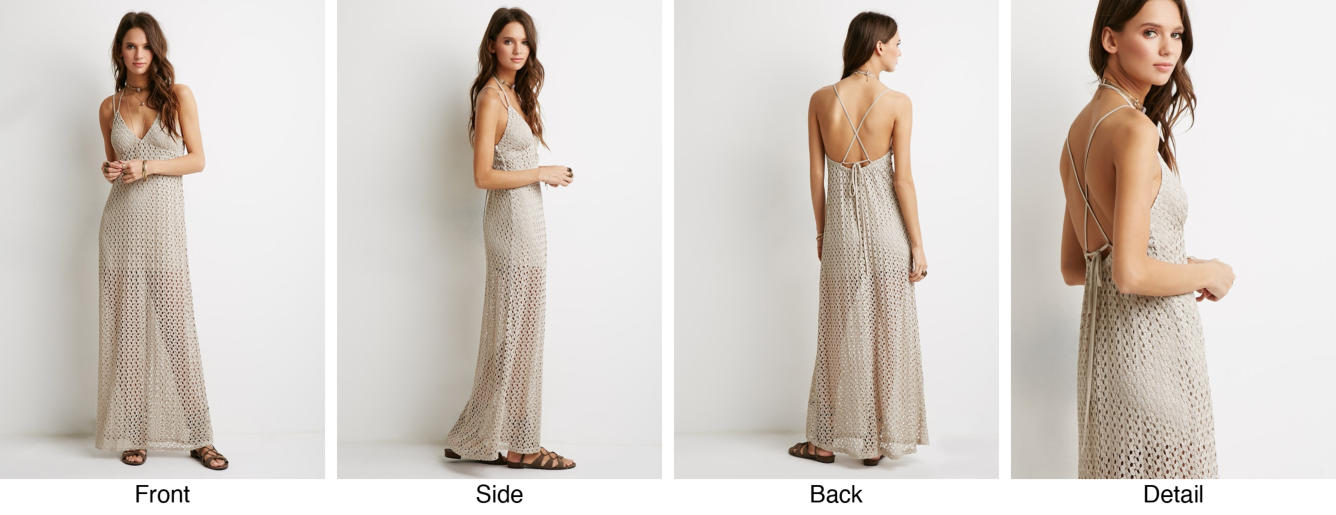
\includegraphics[width=0.92\textwidth]{view_incompleteness.png}
\caption{Một sản phẩm thời trang được hiển thị từ bốn góc nhìn. Đường cổ chữ V sâu chỉ quan sát được ở góc nhìn \emph{Front}, trong khi dây đan chéo hở lưng chỉ quan sát được ở góc nhìn \emph{Back} -- không một ảnh đơn lẻ nào nắm bắt đồng thời cả hai đặc trưng định danh này (nguồn: Hình 1 trong~\cite{yuan2026fashionmv}).}
\label{fig:view_incompleteness}
\end{figure}

Hình~\ref{fig:view_incompleteness} minh hoạ cụ thể vấn đề: nếu chỉ dùng ảnh mặt trước làm ảnh tham khảo, mô hình không thể ``nhìn thấy'' phần dây đan chéo ở lưng để đối chiếu với một văn bản chỉnh sửa có đề cập đến đặc trưng này. Để giải quyết, FashionMV đề xuất định nghĩa lại bài toán ở \textbf{mức sản phẩm} -- \textbf{Multi-View CIR} -- trong đó cả truy vấn lẫn gallery đều là các sản phẩm được biểu diễn bởi toàn bộ tập ảnh đa góc nhìn. Đi kèm định nghĩa bài toán, bài báo công bố bộ dữ liệu FashionMV (127 nghìn sản phẩm, 472 nghìn ảnh, hơn 220 nghìn triplet CIR) và mô hình \textbf{ProCIR} xây dựng trên mô hình ngôn ngữ lớn đa phương thức Qwen3.5-0.8B~\cite{qwen2026qwen35}.

Thực tập 1 chọn bài báo FashionMV làm đối tượng nghiên cứu vì ba lý do chính:
\begin{enumerate}
    \item \textbf{Tính mới của bài toán.} Đây là công trình đầu tiên -- và tại thời điểm khảo sát là duy nhất -- chính thức hoá bài toán CIR ở mức sản phẩm đa góc nhìn. Nắm vững công trình này là nền tảng trực tiếp cho hướng nghiên cứu của học viên ở các giai đoạn tiếp theo.
    \item \textbf{Khả năng tái lập.} Tác giả công bố công khai bộ chú thích (annotation), checkpoint mô hình ProCIR và mã đánh giá, tạo điều kiện kiểm chứng độc lập các kết quả được công bố.
    \item \textbf{Giá trị khoa học của việc kiểm chứng.} Tái lập một công trình mới, sử dụng kiến trúc MLLM lai (\emph{hybrid}) giữa attention tuyến tính và attention đầy đủ, trên hạ tầng tính toán hạn chế giúp làm rõ những yếu tố thực tế (nguồn dữ liệu, độ phân giải ảnh, kích thước gallery, giới hạn GPU) ảnh hưởng đến kết quả đánh giá -- những yếu tố thường không được đề cập trong bài báo gốc. Đây cũng là một vấn đề được cộng đồng học máy quan tâm rộng rãi~\cite{pineau2021reproducibility}.
\end{enumerate}

\section{Mục tiêu của đề tài}

Mục tiêu tổng quát của Thực tập 1 là \emph{nắm vững và kiểm chứng độc lập} công trình FashionMV, từ đó xác định các hạn chế và hướng mở rộng cho giai đoạn nghiên cứu tiếp theo. Cụ thể, đề tài hướng đến ba mục tiêu sau:

\begin{enumerate}
    \item \textbf{Tổng hợp bài báo.} Trình bày lại một cách có hệ thống nội dung bài báo FashionMV: bài toán Multi-View CIR, pipeline xây dựng bộ dữ liệu, kiến trúc và các cơ chế huấn luyện của ProCIR, cùng các kết quả thực nghiệm và phân tích ablation do tác giả công bố. Đặt công trình trong bối cảnh rộng hơn của các nghiên cứu về CIR và biểu diễn đa phương thức.
    \item \textbf{Tái lập thực nghiệm.} Chạy lại quy trình đánh giá của ProCIR bằng checkpoint và mã nguồn công khai của tác giả trên tập validation của FashionMV; đối chiếu kết quả thu được với số liệu được công bố và phân tích nguyên nhân của các sai lệch.
    \item \textbf{Đánh giá mô hình cơ sở.} Triển khai và đánh giá các mô hình cơ sở (baseline) trên cùng thiết lập, nhằm có điểm tham chiếu độc lập để so sánh với ProCIR và kiểm tra tính hợp lý của pipeline đánh giá.
\end{enumerate}

\section{Phạm vi và giới hạn của đề tài}

\paragraph{Phạm vi.} Đề tài tập trung vào giai đoạn \emph{đánh giá} (inference/evaluation) của ProCIR, sử dụng checkpoint 0.8B tốt nhất do tác giả phát hành (cấu hình MT+Align+SFT theo ký hiệu của bài báo). Các mô hình cơ sở được lựa chọn là CLIP ViT-B/32~\cite{radford2021clip} và FashionCLIP~\cite{chia2022fashionclip} trong chế độ zero-shot với chiến lược hợp nhất muộn (\emph{late fusion}). Phép đo đánh giá chính là Recall@K (K = 1, 5, 10), theo đúng giao thức của bài báo.

\paragraph{Giới hạn.} Trong quá trình thực hiện, đề tài gặp một số ràng buộc khách quan định hình phạm vi thực nghiệm:
\begin{itemize}
    \item \textbf{Mã huấn luyện chưa được công bố.} Kho mã nguồn chính thức chỉ cung cấp mã đánh giá và checkpoint (mục ``Training Code -- Coming Soon''), do đó việc tái lập được hiểu là tái lập kết quả đánh giá, không phải huấn luyện lại mô hình từ đầu.
    \item \textbf{Nguồn ảnh.} FashionMV chỉ phát hành chú thích văn bản, không kèm ảnh. Nguồn ảnh gốc của DeepFashion và Fashion200K không tải tự động được, phải thay thế bằng các bản sao (mirror) công khai trên HuggingFace; trang tải chính thức của FashionGen đã ngừng hoạt động nên bộ dữ liệu này nằm ngoài phạm vi đánh giá.
    \item \textbf{Tài nguyên tính toán.} Học viên không có GPU riêng; thực nghiệm ProCIR được chạy trên GPU miễn phí của Kaggle (giới hạn khoảng 12 giờ mỗi phiên và 30 giờ mỗi tuần), dẫn đến việc Fashion200K chỉ được đánh giá trên một mẫu con.
\end{itemize}
Các giới hạn này được trình bày chi tiết và phân tích ảnh hưởng định lượng ở Chương~\ref{chapter:experimental-basis} và Chương~\ref{chapter:experiments}.

\section{Đóng góp của báo cáo}

Ngoài việc tổng hợp bài báo, báo cáo có các đóng góp thực nghiệm sau:
\begin{itemize}
    \item Xây dựng quy trình chuẩn bị dữ liệu ảnh từ nguồn thay thế (parquet trên HuggingFace $\to$ thư mục ảnh theo mã sản phẩm) tương thích với mã đánh giá gốc, cùng thống kê độ phủ ảnh cho từng bộ dữ liệu.
    \item Tái lập kết quả ProCIR trên toàn bộ 5.188 triplet validation của DeepFashion và trên mẫu con 1.500 triplet của Fashion200K; phân tích hai nguồn sai lệch chính theo hai chiều ngược nhau (độ phân giải ảnh và kích thước gallery).
    \item Đánh giá hai baseline zero-shot CLIP và FashionCLIP trên cùng tập triplet và cùng gallery với ProCIR, kèm khảo sát trọng số hợp nhất $\alpha$ và phân tích ảnh hưởng của việc sản phẩm nguồn nằm trong gallery -- một chi tiết của giao thức đánh giá chưa được thảo luận trong bài báo gốc.
\end{itemize}

\section{Cấu trúc báo cáo}

Phần còn lại của báo cáo được tổ chức như sau:
\begin{itemize}
    \item \textbf{Chương~\ref{chapter:overview}} trình bày tổng quan về bài toán truy xuất ảnh có điều kiện: định nghĩa hình thức, lịch sử phát triển, các ứng dụng tiêu biểu và những thách thức còn tồn tại.
    \item \textbf{Chương~\ref{chapter:background}} trình bày cơ sở lý thuyết (Transformer, Vision Transformer, học tương phản, CLIP, mô hình ngôn ngữ lớn đa phương thức, attention tuyến tính) và khảo sát các nghiên cứu liên quan về CIR cũng như biểu diễn đa phương thức trong miền thời trang.
    \item \textbf{Chương~\ref{chapter:method}} trình bày chi tiết phương pháp của bài báo FashionMV: định nghĩa bài toán Multi-View CIR, pipeline xây dựng bộ dữ liệu, kiến trúc ProCIR với ba cơ chế bổ trợ, và các kết quả do tác giả công bố.
    \item \textbf{Chương~\ref{chapter:experimental-basis}} giới thiệu các bộ dữ liệu, giao thức và độ đo đánh giá, cùng quy trình chuẩn bị dữ liệu ảnh thay thế.
    \item \textbf{Chương~\ref{chapter:experiments}} trình bày thiết lập, kết quả tái lập ProCIR, kết quả các mô hình cơ sở và thảo luận.
    \item \textbf{Chương~\ref{chapter:conclusion}} tổng kết kết quả đạt được, những hạn chế tồn tại và định hướng phát triển.
\end{itemize}
 % Giới thiệu đề tài
        \newpage
	\chapter{Tổng quan về bài toán truy xuất ảnh có điều kiện}\label{chapter:overview}
\pagestyle{fancy}

Chương này trình bày bức tranh tổng quan về bài toán truy xuất ảnh có điều kiện (CIR): định nghĩa hình thức và mối quan hệ với các bài toán truy xuất đa phương thức khác, quá trình phát triển của lĩnh vực, các ứng dụng tiêu biểu và những thách thức còn mở -- trong đó có thách thức khiếm khuyết góc nhìn mà bài báo FashionMV hướng tới giải quyết.

\section{Định nghĩa bài toán}\label{sec:problem-definition}

\subsection{Truy xuất thông tin đa phương thức}

Truy xuất thông tin (\emph{information retrieval}) là bài toán tìm trong một tập lớn các đối tượng (gọi là \emph{gallery} hoặc \emph{corpus}) những đối tượng phù hợp nhất với một nhu cầu thông tin được diễn đạt qua truy vấn~\cite{manning2008ir}. Trong các hệ thống truy xuất hiện đại dựa trên học sâu, cả truy vấn và đối tượng trong gallery đều được ánh xạ vào một không gian vector chung (\emph{embedding space}) bởi các hàm mã hoá; mức độ phù hợp được đo bằng độ tương đồng (thường là cosine) giữa các vector; và kết quả truy xuất là danh sách các đối tượng được xếp hạng theo độ tương đồng giảm dần. Cách tiếp cận này cho phép tiền tính toán toàn bộ embedding của gallery và sử dụng các thư viện tìm kiếm lân cận gần đúng như FAISS~\cite{johnson2019faiss} để truy xuất trên hàng triệu đối tượng trong thời gian thực.

Tuỳ theo phương thức (\emph{modality}) của truy vấn và gallery, có thể phân biệt các bài toán:
\begin{itemize}
    \item \textbf{Truy xuất ảnh theo nội dung} (\emph{content-based image retrieval}): truy vấn là ảnh, gallery là ảnh.
    \item \textbf{Truy xuất xuyên phương thức} (\emph{cross-modal retrieval}): truy vấn là văn bản, gallery là ảnh (Text-to-Image, T2I), hoặc ngược lại (Image-to-Text, I2T).
    \item \textbf{Truy xuất ảnh có điều kiện} (CIR): truy vấn là một cặp (ảnh, văn bản), gallery là ảnh. Đây là bài toán \emph{đa phương thức hợp thành}: thông tin trong truy vấn không nằm hoàn toàn ở một phương thức nào, mà là kết quả của việc ``áp dụng'' văn bản lên ảnh.
\end{itemize}

\subsection{Truy xuất ảnh có điều kiện ở mức ảnh}

Trong thiết lập chuẩn, một mẫu dữ liệu CIR là một \emph{triplet} $(I_{ref}, T_{mod}, I_{tgt})$, trong đó $I_{ref}$ là ảnh tham khảo, $T_{mod}$ là văn bản chỉnh sửa mô tả sự khác biệt mong muốn, và $I_{tgt}$ là ảnh đích. Cho một gallery $\mathcal{G} = \{I_1, \dots, I_M\}$, mục tiêu là học hai hàm mã hoá
\begin{equation}
    f_q : (I_{ref}, T_{mod}) \mapsto \mathbf{q} \in \mathbb{R}^d, \qquad f_g : I \mapsto \mathbf{g} \in \mathbb{R}^d
\end{equation}
sao cho ảnh đích được xếp hạng cao nhất theo độ tương đồng:
\begin{equation}
    I_{tgt} = \arg\max_{I \in \mathcal{G}} \; \cos\big(f_q(I_{ref}, T_{mod}),\, f_g(I)\big).
    \label{eq:cir-objective}
\end{equation}

Điểm khó của CIR nằm ở bản chất \emph{hợp thành} của truy vấn: văn bản chỉnh sửa thường mô tả \emph{tương đối} (``dài hơn'', ``đổi sang màu trắng'', ``bỏ túi ngực'') chứ không mô tả đầy đủ ảnh đích, nên mô hình phải đồng thời (i) giữ lại những thuộc tính của ảnh tham khảo không bị đề cập, và (ii) thay đổi đúng những thuộc tính được văn bản yêu cầu. Một phép cộng đơn giản giữa embedding ảnh và embedding văn bản thường không đủ để biểu diễn phép biến đổi này, như sẽ được kiểm chứng bằng thực nghiệm ở Chương~\ref{chapter:experiments}.

\subsection{Truy xuất ảnh có điều kiện ở mức sản phẩm (Multi-View CIR)}

Bài báo FashionMV~\cite{yuan2026fashionmv} tổng quát hoá bài toán trên từ mức ảnh lên \emph{mức sản phẩm}. Mỗi sản phẩm $P$ được biểu diễn bởi một tập ảnh đa góc nhìn
\begin{equation}
    \mathcal{V}^P = \{I^P_1, I^P_2, \dots, I^P_{N_P}\}, \qquad N_P \in [2, 5],
\end{equation}
và một triplet CIR có dạng $(P_{src}, T_{mod}, P_{tgt})$. Gallery bây giờ là một tập sản phẩm, và mô hình phải tổng hợp mọi góc nhìn của mỗi sản phẩm thành một embedding duy nhất:
\begin{equation}
    \mathbf{q} = f_q\big(\mathcal{V}^{P_{src}}, T_{mod}\big), \qquad \mathbf{g}_P = f_g\big(\mathcal{V}^{P}\big).
\end{equation}
Bài toán CIR chuẩn là trường hợp suy biến khi $N_P = 1$. Hình~\ref{fig:cir-vs-mvcir} so sánh trực quan hai thiết lập.

\begin{figure}[h]
\centering
\begin{tikzpicture}[
  img/.style={draw, fill=blue!8, minimum width=0.85cm, minimum height=1.05cm, font=\scriptsize, align=center},
  txt/.style={draw, rounded corners=2pt, fill=orange!12, text width=2.9cm, align=center, font=\scriptsize, minimum height=1.05cm},
  enc/.style={draw, rounded corners=3pt, fill=gray!15, minimum width=1.6cm, minimum height=0.8cm, font=\scriptsize\bfseries, align=center},
  arr/.style={-{Stealth[length=2mm]}, thick},
  lbl/.style={font=\small\bfseries, anchor=west}
]
% ---- (a) image level
\node[lbl] at (-0.6,2.1) {(a) CIR mức ảnh};
\node[img] (a1) at (0,1) {Front};
\node[font=\large] at (0.95,1) {$+$};
\node[txt] (at) at (2.85,1) {``Thêm dây đan chéo hở lưng''};
\node[enc] (ae) at (6.0,1) {$f_q$};
\draw[arr] (at.east) -- (ae.west);
\node[img, fill=green!10] (ag) at (8.9,1) {Ảnh\\[-2pt]đích};
\draw[arr] (ae.east) -- node[above, font=\scriptsize]{truy xuất} (ag.west);
\node[font=\scriptsize, text=red!70!black, align=left, anchor=west] at (9.5,1) {Không thấy\\phần lưng!};
% ---- (b) product level
\node[lbl] at (-0.6,-0.55) {(b) Multi-View CIR mức sản phẩm};
\foreach \v/\x in {Front/0, Back/0.95, Side/1.9} { \node[img] at (\x,-1.7) {\v}; }
\draw[decorate, decoration={brace, amplitude=4pt, mirror}] (-0.45,-2.35) -- (2.35,-2.35) node[midway, below=4pt, font=\scriptsize] {$\mathcal{V}^{P_{src}}$ (2--5 ảnh)};
\node[font=\large] at (2.85,-1.7) {$+$};
\node[txt] (bt) at (4.75,-1.7) {``Thêm dây đan chéo hở lưng''};
\node[enc] (be) at (7.6,-1.7) {$f_q$};
\draw[arr] (bt.east) -- (be.west);
\foreach \x in {9.2, 9.75, 10.3} { \node[img, fill=green!10, minimum width=0.5cm] at (\x,-1.7) {}; }
\draw[arr] (be.east) -- (8.95,-1.7);
\node[font=\scriptsize] at (9.75,-2.5) {Sản phẩm đích $P_{tgt}$};
\end{tikzpicture}
\caption{So sánh CIR mức ảnh và Multi-View CIR mức sản phẩm. Ở (a), chi tiết phần lưng được văn bản đề cập nhưng không có mặt trong ảnh tham khảo; ở (b), toàn bộ góc nhìn của sản phẩm nguồn được đưa vào truy vấn và đích truy xuất là một sản phẩm (tập ảnh) thay vì một ảnh đơn.}
\label{fig:cir-vs-mvcir}
\end{figure}

Việc chuyển lên mức sản phẩm thay đổi bài toán ở ba khía cạnh. Thứ nhất, \textbf{đơn vị truy xuất} trùng với đơn vị kinh doanh: người dùng thương mại điện tử cần tìm một \emph{sản phẩm} để mua chứ không phải một bức ảnh. Thứ hai, \textbf{thông tin thị giác đầy đủ hơn}: các chi tiết phân bố trên nhiều góc nhìn (cổ áo ở mặt trước, khoá kéo ở mặt sau, túi ở mặt bên) đều có mặt trong truy vấn. Thứ ba, \textbf{yêu cầu mới đối với mô hình}: mô hình phải chấp nhận một số lượng ảnh thay đổi và biết tổng hợp thông tin xuyên góc nhìn -- điều mà các kiến trúc CIR một-ảnh không được thiết kế để làm.

\section{Lịch sử phát triển}\label{sec:history}

Sự phát triển của CIR có thể chia thành bốn giai đoạn, gắn liền với sự tiến hoá của các mô hình biểu diễn thị giác--ngôn ngữ nền tảng (Hình~\ref{fig:cir-timeline}).

\begin{figure}[h]
\centering
\begin{tikzpicture}[
  ev/.style={font=\scriptsize, align=center, text width=2.5cm},
  dot/.style={circle, fill=#1, inner sep=2.2pt}
]
\draw[very thick, -{Stealth[length=3mm]}] (0,0) -- (15.4,0);
\foreach \px/\yr/\cl/\ti/\de in {
  0.8/2019/blue/TIRG/{Hợp nhất có giám sát\\(ResNet + LSTM)},
  3.2/2021/blue/{FashionIQ, CIRR}/{Benchmark CIR\\mức ảnh},
  5.6/2022/teal/CLIP4Cir/{Combiner trên\\không gian CLIP},
  8.0/2023/orange/{Pic2Word, SEARLE}/{CIR zero-shot\\(textual inversion)},
  10.4/2024/orange/{LinCIR, SPRC}/{Huấn luyện chỉ văn bản;\\prompt từ BLIP-2},
  12.8/2025/red/CoLLM/{LLM làm\\xương sống},
  14.8/2026/purple/FashionMV/{CIR mức sản phẩm\\đa góc nhìn}} {
  \node[dot=\cl] at (\px,0) {};
  \node[font=\scriptsize\bfseries] at (\px,-0.4) {\yr};
  \node[ev, font=\scriptsize\bfseries, text=\cl!70!black] at (\px,0.95) {\ti};
  \node[ev] at (\px,-1.15) {\de};
}
\end{tikzpicture}
\caption{Các mốc phát triển tiêu biểu của bài toán truy xuất ảnh có điều kiện.}
\label{fig:cir-timeline}
\end{figure}

\paragraph{Giai đoạn 1 -- Hợp nhất đặc trưng có giám sát (2019--2021).} TIRG~\cite{vo2019tirg} là công trình đặt nền móng, sử dụng ResNet~\cite{he2016resnet} để mã hoá ảnh và LSTM để mã hoá văn bản, rồi hợp nhất hai vector bằng một cơ chế \emph{cổng phần dư} (\emph{gated residual}): một nhánh cổng quyết định giữ lại bao nhiêu thông tin từ ảnh gốc, một nhánh phần dư bổ sung sự thay đổi do văn bản yêu cầu. Các công trình tiếp theo cải tiến cơ chế hợp nhất bằng bộ tự mã hoá hợp thành (ComposeAE~\cite{anwaar2021composeae}), học hợp thành kép kết hợp hiệu chỉnh (DCNet~\cite{kim2021dcnet}) hay attention ngữ nghĩa (SAC~\cite{jandial2022sac}). Điểm chung của giai đoạn này là các bộ mã hoá ảnh và văn bản được huấn luyện riêng rẽ, không có không gian biểu diễn chung từ trước, nên mô hình phải học sự căn chỉnh ảnh--văn bản từ chính dữ liệu triplet vốn có quy mô nhỏ.

\paragraph{Giai đoạn 2 -- Kế thừa không gian CLIP (2022--2023).} Sự ra đời của CLIP~\cite{radford2021clip} -- mô hình được tiền huấn luyện tương phản trên 400 triệu cặp ảnh--văn bản -- cung cấp một không gian biểu diễn trong đó ảnh và văn bản đã được căn chỉnh sẵn. CLIP4Cir~\cite{baldrati2022clip4cir} khai thác điều này bằng cách giữ nguyên (hoặc tinh chỉnh nhẹ) hai bộ mã hoá của CLIP và chỉ huấn luyện một mạng \emph{Combiner} nhỏ để kết hợp hai embedding; phương pháp đơn giản này vượt trội đáng kể các mô hình giai đoạn trước và trở thành baseline tiêu chuẩn. SPRC~\cite{bai2024sprc} tiếp tục tận dụng BLIP-2~\cite{li2023blip2} để sinh các prompt mức câu, cải thiện khả năng biểu diễn các chỉnh sửa phức tạp.

\paragraph{Giai đoạn 3 -- CIR không cần triplet gán nhãn (2023--2024).} Gán nhãn triplet CIR rất tốn kém vì người gán nhãn phải viết mô tả sự khác biệt cho từng cặp ảnh. Hướng zero-shot CIR (ZS-CIR) tìm cách loại bỏ chi phí này. Pic2Word~\cite{saito2023pic2word} và SEARLE~\cite{baldrati2023searle} học một ánh xạ biến ảnh thành một ``từ giả'' (\emph{pseudo-word token}) trong không gian token của bộ mã hoá văn bản CLIP, sau đó ghép từ giả với văn bản chỉnh sửa thành một câu hoàn chỉnh (ví dụ ``\emph{a photo of [$S_*$] with short sleeves}'') để mã hoá thành truy vấn. LinCIR~\cite{gu2024lincir} chỉ huấn luyện trên văn bản thông qua phép chiếu tự che (\emph{self-masking projection}); SLERP+TAT~\cite{jang2024slerp} hợp nhất hai embedding bằng nội suy tuyến tính cầu; CompoDiff~\cite{gu2024compodiff} sử dụng mô hình khuếch tán tiềm ẩn để sinh embedding đích.

\paragraph{Giai đoạn 4 -- Mô hình ngôn ngữ lớn (2025--nay).} Các mô hình ngôn ngữ lớn đa phương thức (MLLM) có khả năng hiểu ngôn ngữ và suy luận vượt trội so với bộ mã hoá văn bản của CLIP. CoLLM~\cite{huynh2025collm} sử dụng LLM làm xương sống để tạo embedding hợp nhất ảnh--văn bản. Song song, lĩnh vực mở rộng sang ngữ nghĩa chi tiết (FineCIR~\cite{li2025finecir}), tương tác nhiều lượt (MAI~\cite{chen2025mai}) và miền video (EgoCVR~\cite{hummel2024egocvr}). Bài báo FashionMV~\cite{yuan2026fashionmv} thuộc giai đoạn này, và là công trình đầu tiên thay đổi \emph{phía đầu vào thị giác} vốn không đổi suốt bảy năm: từ một ảnh tham khảo sang toàn bộ tập ảnh đa góc nhìn của sản phẩm.

\section{Các ứng dụng tiêu biểu}\label{sec:applications}

CIR có nhiều ứng dụng thực tiễn, đặc biệt trong các lĩnh vực mà người dùng khó diễn đạt nhu cầu bằng từ khoá:

\begin{itemize}
    \item \textbf{Tìm kiếm sản phẩm thương mại điện tử.} Đây là ứng dụng trực tiếp nhất: người dùng chọn một sản phẩm đang xem và mô tả bằng ngôn ngữ tự nhiên những điểm muốn thay đổi. Bộ dữ liệu FashionIQ~\cite{wu2021fashioniq} được xây dựng chính từ kịch bản phản hồi của người mua sắm thời trang. Với Multi-View CIR, truy vấn có thể dùng toàn bộ ảnh của trang sản phẩm thay vì buộc người dùng chọn một ảnh.
    \item \textbf{Tìm kiếm tương tác và hội thoại.} Trong các hệ thống trợ lý mua sắm, người dùng tinh chỉnh kết quả qua nhiều lượt (``tối màu hơn'', ``không có hoạ tiết''). Mỗi lượt là một bài toán CIR với ảnh tham khảo là kết quả của lượt trước~\cite{chen2025mai}. Kiến trúc hội thoại hai lượt của ProCIR còn cho phép lưu cache trạng thái của lượt nhận thức thị giác để giảm độ trễ cho các lượt chỉnh sửa tiếp theo (Mục~\ref{sec:two-stage}).
    \item \textbf{Thiết kế và sáng tạo.} Nhà thiết kế thời trang có thể tìm các mẫu tham khảo bằng cách mô tả biến thể của một thiết kế sẵn có, hoặc kiểm tra xem một ý tưởng đã tồn tại trong danh mục hay chưa.
    \item \textbf{Gợi ý sản phẩm thay thế.} Khi một sản phẩm hết hàng, hệ thống có thể tìm các sản phẩm tương tự nhưng khác ở một thuộc tính cụ thể (size, màu, chất liệu).
    \item \textbf{Các miền ngoài thời trang.} CIR trên ảnh miền mở (CIRR~\cite{liu2021cirr}), truy xuất video từ góc nhìn thứ nhất (EgoCVR~\cite{hummel2024egocvr}), và -- như bài báo FashionMV gợi ý -- các miền thương mại điện tử đa góc nhìn khác như nội thất và đồ điện tử.
\end{itemize}

\section{Những thách thức và hướng nghiên cứu}\label{sec:challenges}

Mặc dù đạt nhiều tiến bộ, CIR vẫn đối mặt với những thách thức lớn:

\paragraph{(1) Khiếm khuyết góc nhìn.} Như đã phân tích ở Chương~\ref{chapter:introduction}, giả định một-ảnh khiến mô hình thiếu thông tin khi văn bản chỉnh sửa đề cập đến chi tiết không quan sát được. Các công trình biểu diễn thời trang như FashionViL~\cite{han2022fashionvil} đã nhận ra giá trị của dữ liệu đa góc nhìn, nhưng chỉ dùng nó như một dạng tăng cường dữ liệu khi tiền huấn luyện; lúc truy xuất, mô hình vẫn hoạt động trên từng ảnh riêng lẻ. Đây là khoảng trống mà FashionMV giải quyết.

\paragraph{(2) Tổng hợp thông tin xuyên góc nhìn.} Ngay cả khi có nhiều ảnh, câu hỏi \emph{tổng hợp như thế nào} vẫn mở. Các chiến lược đơn giản như lấy trung bình embedding (MeanPool) có thể làm loãng chi tiết đặc thù của từng góc nhìn; chọn cặp góc nhìn khớp nhất (MaxSim) lại thất bại khi văn bản đề cập các thuộc tính phân bố trên nhiều góc nhìn. Mã hoá đồng thời mọi góc nhìn (Joint) đòi hỏi mô hình có khả năng hiểu đa ảnh tốt, và có thể phản tác dụng với các mô hình yếu (Mục~\ref{sec:paper-results}).

\paragraph{(3) Dữ liệu gán nhãn và tính mơ hồ.} Triplet CIR do con người viết tốn kém và nhiễu; triplet tự động sinh bởi mô hình lại có nguy cơ ảo giác (\emph{hallucination}). Một vấn đề khác là \emph{mơ hồ đa đáp án đúng} (\emph{multi-positive ambiguity}): văn bản chỉnh sửa ngắn thường phù hợp với nhiều sản phẩm trong gallery, trong khi giao thức đánh giá chỉ công nhận một đích duy nhất. CIRCO~\cite{baldrati2023searle} giảm thiểu vấn đề này bằng cách gán nhiều đáp án đúng cho mỗi truy vấn; FashionMV giảm thiểu nó ngay từ khâu sinh dữ liệu bằng cách cho MLLM đối chiếu đích với nhiều ứng viên cạnh tranh (Mục~\ref{sec:dataset-construction}).

\paragraph{(4) Chi phí tính toán và độ trễ.} Các mô hình dựa trên MLLM có độ chính xác cao nhưng tốn kém hơn nhiều so với các mô hình kiểu CLIP, đặc biệt khi mỗi truy vấn chứa nhiều ảnh. Đây là một rào cản thực tế, như chính quá trình tái lập trong báo cáo này cho thấy (Chương~\ref{chapter:experiments}).

\paragraph{(5) Tính tái lập và giao thức đánh giá.} Kết quả CIR phụ thuộc mạnh vào các chi tiết của giao thức: kích thước gallery, việc có loại sản phẩm nguồn khỏi kết quả xếp hạng hay không, độ phân giải ảnh, phiên bản văn bản chỉnh sửa (ngắn hay dài). Những chi tiết này hiếm khi được nêu đầy đủ, khiến việc so sánh giữa các công trình trở nên khó khăn. Báo cáo này đưa ra các phân tích định lượng cụ thể về ảnh hưởng của hai yếu tố đầu tiên (Mục~\ref{sec:discussion}).

\paragraph{Hướng nghiên cứu.} Từ các thách thức trên, các hướng nghiên cứu nổi bật hiện nay bao gồm: thiết kế cơ chế tổng hợp đa góc nhìn hiệu quả và có khả năng diễn giải (ví dụ biết góc nhìn nào liên quan đến chi tiết nào trong văn bản chỉnh sửa); tận dụng MLLM cỡ nhỏ để cân bằng độ chính xác và chi phí; tiêm tri thức miền (\emph{domain knowledge}) thông qua chú thích có cấu trúc; và xây dựng giao thức đánh giá bền vững hơn với hiện tượng đa đáp án đúng.
 % Tổng quan bài toán CIR
        \newpage
	\chapter{Cơ sở lý thuyết và các nghiên cứu liên quan}\label{chapter:background}
\pagestyle{fancy}

Chương này trình bày các kiến thức nền tảng cần thiết để hiểu phương pháp ProCIR và các mô hình cơ sở được đánh giá trong báo cáo. Mục~\ref{sec:architectures} điểm lại các kiến trúc học sâu nền tảng: Transformer, Vision Transformer và các biến thể attention tuyến tính được dùng trong Qwen3.5. Mục~\ref{sec:contrastive} trình bày học biểu diễn tương phản và mô hình CLIP. Mục~\ref{sec:mllm} trình bày mô hình ngôn ngữ lớn đa phương thức và cách sử dụng chúng như bộ mã hoá embedding. Mục~\ref{sec:related-cir} và Mục~\ref{sec:related-datasets} khảo sát các phương pháp và bộ dữ liệu CIR liên quan.

\section{Các kiến trúc học sâu nền tảng}\label{sec:architectures}

\subsection{Kiến trúc Transformer và cơ chế self-attention}

Transformer~\cite{vaswani2017attention} là kiến trúc nền tảng của hầu hết các mô hình ngôn ngữ và thị giác--ngôn ngữ hiện đại. Thành phần cốt lõi của Transformer là cơ chế \emph{self-attention}, cho phép mỗi phần tử trong chuỗi tổng hợp thông tin từ mọi phần tử khác theo trọng số được học. Cho chuỗi đầu vào $\mathbf{X} \in \mathbb{R}^{n \times d}$ gồm $n$ token, mỗi token có chiều $d$, ba ma trận truy vấn (\emph{query}), khoá (\emph{key}) và giá trị (\emph{value}) được tính bằng các phép chiếu tuyến tính:
\begin{equation}
    \mathbf{Q} = \mathbf{X}\mathbf{W}_Q, \quad \mathbf{K} = \mathbf{X}\mathbf{W}_K, \quad \mathbf{V} = \mathbf{X}\mathbf{W}_V.
\end{equation}
Đầu ra của attention là tổ hợp có trọng số của các vector giá trị, với trọng số được chuẩn hoá bằng hàm softmax:
\begin{equation}
    \mathrm{Attention}(\mathbf{Q}, \mathbf{K}, \mathbf{V}) = \mathrm{softmax}\!\left(\frac{\mathbf{Q}\mathbf{K}^\top}{\sqrt{d_k}} + \mathbf{M}\right)\mathbf{V},
    \label{eq:attention}
\end{equation}
trong đó $d_k$ là chiều của vector khoá và $\mathbf{M}$ là ma trận mặt nạ. Trong các mô hình ngôn ngữ tự hồi quy (\emph{decoder-only}), $\mathbf{M}$ là \textbf{mặt nạ nhân quả} (\emph{causal mask}): $M_{ij} = 0$ nếu $j \le i$ và $M_{ij} = -\infty$ nếu $j > i$, tức là mỗi token chỉ được ``nhìn'' các token đứng trước nó. Tính chất nhân quả này đóng vai trò then chốt trong thiết kế hội thoại hai lượt của ProCIR: embedding được trích ở cuối lượt thứ nhất hoàn toàn không bị ảnh hưởng bởi nội dung của lượt thứ hai (Mục~\ref{sec:two-stage}).

\textbf{Multi-head attention} thực hiện $h$ phép attention song song trên các không gian con khác nhau rồi ghép kết quả, cho phép mô hình đồng thời nắm bắt nhiều kiểu quan hệ. Các biến thể hiện đại như \emph{grouped-query attention} cho nhiều đầu truy vấn dùng chung một cặp khoá--giá trị để giảm bộ nhớ đệm (KV cache) khi suy luận. Mỗi tầng Transformer gồm một khối attention và một mạng truyền thẳng (\emph{feed-forward network}), mỗi khối đều có kết nối phần dư và chuẩn hoá tầng. Để mã hoá thông tin vị trí, các mô hình gần đây sử dụng \emph{rotary position embedding} (RoPE)~\cite{su2024rope}, xoay các vector truy vấn và khoá theo một góc phụ thuộc vị trí.

Độ phức tạp tính toán của attention~\eqref{eq:attention} là $\mathcal{O}(n^2 d)$ theo độ dài chuỗi. Với đầu vào đa phương thức nhiều ảnh -- mỗi ảnh có thể tạo ra hàng trăm token -- chi phí bậc hai này trở thành nút thắt đáng kể, là động lực cho các kiến trúc attention tuyến tính ở Mục~\ref{sec:linear-attn}.

\subsection{Vision Transformer}

Vision Transformer (ViT)~\cite{dosovitskiy2021vit} áp dụng trực tiếp Transformer cho ảnh bằng cách chia ảnh $H \times W$ thành lưới các mảnh (\emph{patch}) kích thước $P \times P$, làm phẳng và chiếu tuyến tính mỗi mảnh thành một token. Một ảnh $224 \times 224$ với $P = 32$ (như CLIP ViT-B/32) tạo ra $7 \times 7 = 49$ token, cộng thêm một token \texttt{[CLS]} có trạng thái ẩn cuối cùng được dùng làm biểu diễn toàn cục của ảnh. ViT có ít thiên kiến quy nạp (\emph{inductive bias}) hơn mạng tích chập, nên cần dữ liệu tiền huấn luyện lớn, nhưng khi đủ dữ liệu lại có khả năng mở rộng tốt và trở thành bộ mã hoá ảnh chuẩn trong các mô hình thị giác--ngôn ngữ.

Một điểm quan trọng đối với báo cáo này là \textbf{số token thị giác tỷ lệ với độ phân giải ảnh}. Các MLLM hiện đại như họ Qwen-VL~\cite{wang2024qwen2vl} hỗ trợ \emph{độ phân giải động}: ảnh được giữ gần tỷ lệ gốc và chia thành số mảnh tương ứng, thay vì luôn bị thu về một kích thước cố định. Do đó, ảnh độ phân giải thấp cung cấp ít token -- và ít chi tiết -- hơn cho mô hình ngôn ngữ phía sau. Hệ quả định lượng của tính chất này lên kết quả tái lập được phân tích ở Mục~\ref{sec:discussion}.

\subsection{Attention tuyến tính và kiến trúc lai}\label{sec:linear-attn}

\textbf{Attention tuyến tính}~\cite{katharopoulos2020linear} thay hàm softmax trong~\eqref{eq:attention} bằng tích của các ánh xạ đặc trưng $\phi(\cdot)$, cho phép đổi thứ tự phép nhân ma trận. Với mặt nạ nhân quả, đầu ra tại vị trí $t$ có thể viết dưới dạng hồi quy:
\begin{equation}
    \mathbf{S}_t = \mathbf{S}_{t-1} + \mathbf{v}_t\,\phi(\mathbf{k}_t)^\top, \qquad \mathbf{o}_t = \mathbf{S}_t\,\phi(\mathbf{q}_t),
\end{equation}
trong đó $\mathbf{S}_t \in \mathbb{R}^{d_v \times d_k}$ là một ma trận trạng thái kích thước cố định. Chi phí mỗi bước là hằng số theo độ dài chuỗi, nên toàn chuỗi có độ phức tạp tuyến tính $\mathcal{O}(n)$ thay vì bậc hai. Nhược điểm của dạng cộng dồn đơn giản này là trạng thái ``nhớ mãi'' mọi thứ, dễ bị bão hoà khi chuỗi dài.

Các mô hình không gian trạng thái chọn lọc như Mamba~\cite{gu2023mamba} và các biến thể dùng \emph{quy tắc delta} khắc phục nhược điểm trên bằng cơ chế quên và ghi đè có chọn lọc. \textbf{Gated DeltaNet}~\cite{yang2025gateddeltanet} kết hợp cổng suy giảm $\alpha_t \in (0,1)$ với quy tắc delta:
\begin{equation}
    \mathbf{S}_t = \alpha_t\,\mathbf{S}_{t-1}\big(\mathbf{I} - \beta_t\,\mathbf{k}_t\mathbf{k}_t^\top\big) + \beta_t\,\mathbf{v}_t\mathbf{k}_t^\top,
\end{equation}
trong đó $\beta_t$ là ``tốc độ ghi''. Cổng $\alpha_t$ cho phép xoá nhanh thông tin cũ, còn quy tắc delta cho phép cập nhật chính xác giá trị gắn với một khoá cụ thể.

Vì attention tuyến tính kém attention đầy đủ ở các tác vụ đòi hỏi truy hồi chính xác, nhiều mô hình gần đây chọn \textbf{kiến trúc lai}: xen kẽ phần lớn tầng attention tuyến tính với một số ít tầng attention đầy đủ. Qwen3.5~\cite{qwen2026qwen35} -- mô hình nền của ProCIR -- theo thiết kế này. Đọc trực tiếp tệp cấu hình của checkpoint ProCIR cho thấy 24 tầng của mô hình được bố trí theo chu kỳ \emph{ba tầng attention tuyến tính, một tầng attention đầy đủ} (tham số \texttt{full\_attention\_interval = 4}), tức 18 tầng tuyến tính và 6 tầng đầy đủ, với các tầng tuyến tính có một phép tích chập nhân quả ngắn (\texttt{linear\_conv\_kernel\_dim = 4}). Việc thực thi hiệu quả các tầng tuyến tính đòi hỏi các kernel CUDA chuyên dụng (thư viện \texttt{flash-linear-attention} và \texttt{causal-conv1d}); khi các kernel này không khả dụng, mô hình quay về triển khai tham chiếu bằng PyTorch thuần với tốc độ chậm hơn nhiều -- một yếu tố ảnh hưởng trực tiếp đến quá trình tái lập (Chương~\ref{chapter:experiments}).

\section{Học biểu diễn tương phản đa phương thức}\label{sec:contrastive}

\subsection{Hàm mất mát InfoNCE}

Học tương phản (\emph{contrastive learning}) học không gian biểu diễn bằng cách kéo các cặp mẫu dương (có liên quan) lại gần nhau và đẩy các cặp mẫu âm ra xa. Hàm mất mát phổ biến nhất là \textbf{InfoNCE}~\cite{oord2018cpc}. Cho một batch gồm $B$ cặp $(\mathbf{x}_i, \mathbf{y}_i)$ đã chuẩn hoá $L_2$, với $\mathbf{y}_i$ là mẫu dương của $\mathbf{x}_i$ và mọi $\mathbf{y}_j$ ($j \ne i$) là mẫu âm:
\begin{equation}
    \mathcal{L}_{\mathrm{InfoNCE}}(\mathbf{x}, \mathbf{y}) = -\frac{1}{B}\sum_{i=1}^{B} \log \frac{\exp(\mathbf{x}_i^\top \mathbf{y}_i / \tau)}{\sum_{j=1}^{B}\exp(\mathbf{x}_i^\top \mathbf{y}_j / \tau)},
    \label{eq:infonce}
\end{equation}
trong đó $\tau > 0$ là tham số nhiệt độ (\emph{temperature}) điều khiển độ ``sắc'' của phân phối. Về bản chất, đây là hàm cross-entropy cho bài toán phân loại $B$ lớp: với mỗi $\mathbf{x}_i$, mô hình phải nhận ra đúng $\mathbf{y}_i$ trong số $B$ ứng viên. Kỹ thuật dùng các mẫu khác trong cùng batch làm mẫu âm (\emph{in-batch negatives}) giúp tránh chi phí khai thác mẫu âm riêng; batch càng lớn thì càng nhiều mẫu âm và tín hiệu học càng mạnh~\cite{chen2020simclr}. Khi huấn luyện phân tán, các embedding thường được tập hợp (\emph{all-gather}) từ mọi GPU để tăng số mẫu âm hiệu dụng.

Phiên bản \textbf{đối xứng} lấy trung bình hai chiều $\mathbf{x} \to \mathbf{y}$ và $\mathbf{y} \to \mathbf{x}$:
\begin{equation}
    \mathrm{SymInfoNCE}(\mathbf{x}, \mathbf{y}, \tau) = \tfrac{1}{2}\big[\mathcal{L}_{\mathrm{InfoNCE}}(\mathbf{x}, \mathbf{y}) + \mathcal{L}_{\mathrm{InfoNCE}}(\mathbf{y}, \mathbf{x})\big].
    \label{eq:syminfonce}
\end{equation}
Đây chính là hàm mất mát được sử dụng cho mọi thành phần huấn luyện tương phản của ProCIR (Mục~\ref{sec:procir-objective}).

\subsection{Mô hình CLIP}

CLIP (\emph{Contrastive Language--Image Pre-training})~\cite{radford2021clip} gồm hai bộ mã hoá độc lập -- một bộ mã hoá ảnh (ResNet hoặc ViT) và một bộ mã hoá văn bản (Transformer) -- được huấn luyện đồng thời bằng hàm SymInfoNCE~\eqref{eq:syminfonce} trên khoảng 400 triệu cặp ảnh--chú thích thu thập từ Internet (Hình~\ref{fig:clip}). Sau huấn luyện, ảnh và văn bản có cùng ngữ nghĩa nằm gần nhau trong một không gian embedding chung, cho phép thực hiện truy xuất xuyên phương thức và phân loại zero-shot (so khớp ảnh với các câu dạng ``\emph{a photo of a [class]}'').

\begin{figure}[h]
\centering
\begin{tikzpicture}[
  box/.style={draw, rounded corners=3pt, minimum height=0.8cm, align=center, font=\scriptsize},
  arr/.style={-{Stealth[length=2mm]}, thick}
]
\node[box, fill=blue!10, minimum width=2.4cm] (img) at (0,1.6) {Ảnh $I_1,\dots,I_B$};
\node[box, fill=orange!15, minimum width=2.4cm] (txt) at (0,-1.6) {Văn bản $T_1,\dots,T_B$};
\node[box, fill=blue!25, minimum width=2.2cm] (ie) at (3.2,1.6) {Bộ mã hoá ảnh\\(ViT-B/32)};
\node[box, fill=orange!30, minimum width=2.2cm] (te) at (3.2,-1.6) {Bộ mã hoá\\văn bản};
\draw[arr] (img) -- (ie); \draw[arr] (txt) -- (te);
% matrix
\def\s{0.55}
\foreach \i in {1,...,4} {
  \node[draw, fill=blue!15, minimum size=\s cm, font=\tiny, inner sep=0] at (6.3+\i*\s,2.2) {$I_\i$};
  \node[draw, fill=orange!20, minimum size=\s cm, font=\tiny, inner sep=0] at (6.3,1.65-\i*\s) {$T_\i$};
  \foreach \j in {1,...,4} {
    \ifnum\i=\j
      \node[draw, fill=green!40, minimum size=\s cm, inner sep=0] at (6.3+\i*\s,1.65-\j*\s) {};
    \else
      \node[draw, fill=gray!8, minimum size=\s cm, inner sep=0] at (6.3+\i*\s,1.65-\j*\s) {};
    \fi
  }
}
\draw[arr] (ie.east) -- (6.5,2.2);
\draw[arr] (te.east) -- (6.0,-0.5);
\node[font=\scriptsize, align=left, anchor=west] at (9.2,0.3) {Ma trận tương đồng\\$\mathbf{I}_i^\top \mathbf{T}_j / \tau$:\\\textcolor{green!50!black}{đường chéo} = cặp dương,\\còn lại = cặp âm};
\end{tikzpicture}
\caption{Sơ đồ huấn luyện tương phản của CLIP: hai bộ mã hoá độc lập ánh xạ ảnh và văn bản vào không gian chung; hàm SymInfoNCE tối đa hoá độ tương đồng trên đường chéo của ma trận tương đồng trong batch.}
\label{fig:clip}
\end{figure}

Phiên bản \textbf{CLIP ViT-B/32} được dùng làm baseline trong báo cáo có bộ mã hoá ảnh là ViT-Base với patch kích thước $32 \times 32$ trên ảnh đầu vào $224 \times 224$, và không gian embedding chung 512 chiều. Vì hai bộ mã hoá độc lập, CLIP không có cơ chế tự nhiên để \emph{kết hợp} một ảnh và một văn bản thành một truy vấn; cách đơn giản nhất là hợp nhất muộn (\emph{late fusion}) bằng tổng có trọng số hai embedding -- chính là chiến lược baseline ở Chương~\ref{chapter:experiments}.

\subsection{FashionCLIP}

CLIP được huấn luyện trên dữ liệu Internet tổng quát nên thiếu hiểu biết về các khái niệm thời trang chi tiết (tên kiểu dáng, chất liệu, chi tiết may). \textbf{FashionCLIP}~\cite{chia2022fashionclip} tinh chỉnh CLIP trên dữ liệu danh mục sản phẩm của một nhà bán lẻ thời trang trực tuyến lớn (khoảng 800 nghìn sản phẩm, mỗi sản phẩm gồm ảnh và mô tả văn bản), giữ nguyên kiến trúc ViT-B/32. Kết quả là một mô hình có cùng giao diện sử dụng với CLIP nhưng biểu diễn tốt hơn đáng kể cho các tác vụ thời trang như truy xuất sản phẩm và phân loại thuộc tính. Đánh giá FashionCLIP bên cạnh CLIP cho phép tách bạch lợi ích của \emph{thích nghi miền} (\emph{domain adaptation}) với lợi ích của \emph{kiến trúc CIR chuyên biệt}.

\section{Mô hình ngôn ngữ lớn đa phương thức}\label{sec:mllm}

\subsection{Kiến trúc chung}

Mô hình ngôn ngữ lớn đa phương thức (MLLM) mở rộng một LLM để tiếp nhận thêm đầu vào thị giác. Kiến trúc phổ biến nhất -- được phổ biến bởi BLIP-2~\cite{li2023blip2} và LLaVA~\cite{liu2023llava} -- gồm ba thành phần (Hình~\ref{fig:mllm}): (i) một \textbf{bộ mã hoá thị giác} (thường là ViT) biến ảnh thành chuỗi đặc trưng mảnh; (ii) một \textbf{bộ kết nối} (\emph{projector/merger}) chiếu các đặc trưng này sang không gian embedding token của LLM, đồng thời có thể gộp các mảnh lân cận để giảm số token; (iii) một \textbf{LLM decoder-only} xử lý chuỗi xen kẽ token thị giác và token văn bản bằng attention nhân quả. Mô hình được huấn luyện qua nhiều giai đoạn, trong đó giai đoạn \emph{tinh chỉnh theo chỉ dẫn} (\emph{instruction tuning}) dạy mô hình tuân theo định dạng hội thoại nhiều lượt giữa \texttt{user} và \texttt{assistant}.

\begin{figure}[h]
\centering
\begin{tikzpicture}[
  box/.style={draw, rounded corners=3pt, minimum height=0.85cm, align=center, font=\scriptsize},
  tok/.style={draw, minimum width=0.32cm, minimum height=0.42cm, inner sep=0pt},
  arr/.style={-{Stealth[length=2mm]}, thick}
]
\node[box, fill=blue!8, minimum width=1.5cm] (im) at (0,0) {Ảnh đa\\góc nhìn};
\node[box, fill=blue!25, minimum width=2.0cm] (ve) at (2.4,0) {Bộ mã hoá\\thị giác (ViT)};
\node[box, fill=teal!20, minimum width=1.6cm] (pj) at (4.85,0) {Bộ kết nối\\(gộp $2\times2$)};
\draw[arr] (im) -- (ve); \draw[arr] (ve) -- (pj);
\foreach \k in {0,...,5} { \node[tok, fill=blue!30] at (6.5+\k*0.34,0) {}; }
\foreach \k in {0,...,3} { \node[tok, fill=orange!40] at (8.6+\k*0.34,0) {}; }
\node[tok, fill=red!50] at (10.05,0) {};
\draw[arr] (pj) -- (6.3,0);
\node[font=\tiny, align=center] at (7.35,-0.55) {token thị giác};
\node[font=\tiny, align=center] at (9.1,-0.55) {token văn bản};
\node[font=\tiny, text=red!60!black] at (10.05,0.5) {\texttt{<emb>}};
\node[box, fill=gray!15, minimum width=4.6cm] (llm) at (7.9,1.55) {LLM decoder-only (attention nhân quả)};
\draw[arr] (7.9,0.3) -- (llm.south);
\node[box, fill=red!12] (e) at (11.9,1.55) {Trạng thái ẩn\\tại \texttt{<emb>} $\to \mathbf{e}$};
\draw[arr] (llm.east) -- (e.west);
\end{tikzpicture}
\caption{Kiến trúc chung của một MLLM và cách trích xuất embedding từ trạng thái ẩn tại một token đặc biệt.}
\label{fig:mllm}
\end{figure}

Họ Qwen-VL~\cite{wang2024qwen2vl} có hai đặc điểm liên quan trực tiếp đến báo cáo: \emph{độ phân giải động} (số token thị giác thay đổi theo kích thước ảnh trong một khoảng số điểm ảnh tối thiểu--tối đa) và \emph{M-RoPE} (RoPE đa chiều, mã hoá riêng vị trí theo thời gian, chiều cao và chiều rộng cho token thị giác). Nhờ đó, một yêu cầu có thể chứa nhiều ảnh với kích thước khác nhau.

\subsection{Mô hình nền Qwen3.5-0.8B}

ProCIR sử dụng Qwen3.5-0.8B~\cite{qwen2026qwen35} -- phiên bản nhỏ nhất của họ Qwen3.5, được thiết kế như một mô hình đa phương thức nguyên bản (\emph{native multimodal}). Bảng~\ref{tab:qwen35-config} tóm tắt các siêu tham số kiến trúc, được đọc trực tiếp từ tệp \texttt{config.json} của checkpoint ProCIR do tác giả phát hành.

\begin{table}[h]
\centering
\caption{Cấu hình kiến trúc Qwen3.5-0.8B trong checkpoint ProCIR (đọc từ \texttt{config.json}).}
\label{tab:qwen35-config}
\begin{tabular}{llr}
\toprule
Thành phần & Tham số & Giá trị \\
\midrule
\multirow{8}{*}{Mô hình ngôn ngữ}
 & Số tầng & 24 \\
 & Bố trí tầng & 3 tuyến tính : 1 đầy đủ (18 + 6) \\
 & Chiều ẩn & 1024 \\
 & Chiều tầng truyền thẳng & 3584 \\
 & Số đầu attention (truy vấn / khoá--giá trị) & 8 / 2 \\
 & Chiều mỗi đầu & 256 \\
 & Kích thước từ vựng & 248.320 \\
 & Mã hoá vị trí & M-RoPE, $\theta = 10^7$ \\
\midrule
\multirow{5}{*}{Bộ mã hoá thị giác}
 & Số tầng ViT & 12 \\
 & Chiều ẩn / số đầu & 768 / 12 \\
 & Kích thước patch & $16 \times 16$ \\
 & Hệ số gộp không gian & $2 \times 2$ \\
 & Chiều đầu ra (sang LLM) & 1024 \\
\bottomrule
\end{tabular}
\end{table}

Với patch $16 \times 16$ và hệ số gộp $2 \times 2$, mỗi token thị giác đưa vào LLM tương ứng với một vùng $32 \times 32$ điểm ảnh. Mã nguồn đánh giá của ProCIR giới hạn số điểm ảnh mỗi ảnh trong khoảng $128^2$ đến $512^2$; một ảnh $512 \times 512$ do đó tạo ra $16 \times 16 = 256$ token, và một sản phẩm năm góc nhìn có thể chiếm tới khoảng 1.280 token thị giác. Đây là lý do việc xử lý đa góc nhìn bằng MLLM tốn kém hơn nhiều so với CLIP (49 token mỗi ảnh), và là động lực cho kiến trúc attention lai đã trình bày ở Mục~\ref{sec:linear-attn}.

\subsection{MLLM làm bộ mã hoá embedding}

MLLM vốn được thiết kế để \emph{sinh} văn bản chứ không phải tạo vector biểu diễn. Một hướng nghiên cứu gần đây chuyển hoá MLLM thành bộ mã hoá embedding đa phương thức. E5-V~\cite{jiang2024e5v} dùng prompt dạng ``\emph{tóm tắt nội dung trên trong một từ}'' và lấy trạng thái ẩn của token cuối cùng làm embedding; VLM2Vec~\cite{jiang2025vlm2vec} huấn luyện tương phản MLLM trên một tập lớn các tác vụ embedding; Qwen3-VL-Embedding~\cite{li2026qwen3vlemb} và RzenEmbed~\cite{jian2025rzenembed} là các mô hình embedding đa phương thức đa dụng cỡ 2B--8B tham số, hỗ trợ đầu vào nhiều ảnh. Cơ chế chung là: (i) gắn một token đặc biệt vào cuối chuỗi đầu vào; (ii) nhờ attention nhân quả, trạng thái ẩn ở tầng cuối tại vị trí token này đã ``nhìn thấy'' toàn bộ đầu vào nên có thể dùng làm biểu diễn tổng hợp; (iii) huấn luyện tương phản để không gian này phù hợp cho truy xuất. ProCIR áp dụng đúng cơ chế này với token \texttt{<emb>} (Mục~\ref{sec:procir-embedding}), và các mô hình embedding kể trên là các baseline mạnh nhất trong bài báo FashionMV.

\subsection{Chuỗi suy luận và tinh chỉnh có giám sát}

\textbf{Chain-of-Thought} (CoT)~\cite{wei2022cot} là kỹ thuật cho LLM sinh các bước suy luận trung gian trước khi đưa ra câu trả lời, giúp cải thiện đáng kể khả năng suy luận nhiều bước. Các MLLM gần đây (trong đó có Qwen3.5) tích hợp sẵn định dạng khối \texttt{<think>...</think>} cho phần suy luận trong lượt trả lời của assistant. ProCIR tận dụng khối này theo một cách khác thường: không phải để sinh suy luận, mà để \emph{tiêm} chú thích sản phẩm vào ngữ cảnh khi huấn luyện, rồi loại bỏ dần (Mục~\ref{sec:procir-cot}).

\textbf{Tinh chỉnh có giám sát} (SFT) là việc tiếp tục huấn luyện mô hình với hàm mất mát mô hình hoá ngôn ngữ tự hồi quy trên dữ liệu chuyên biệt, nhằm tiêm tri thức miền hoặc dạy một định dạng đầu ra mới. Trong ProCIR, SFT được dùng như một giai đoạn tiền huấn luyện tuỳ chọn để mô hình ``hiểu'' sản phẩm thời trang trước khi được huấn luyện tương phản.

\section{Các phương pháp truy xuất ảnh có điều kiện liên quan}\label{sec:related-cir}

\subsection{Hợp nhất đặc trưng có giám sát}

TIRG~\cite{vo2019tirg} biểu diễn truy vấn bằng tổ hợp của một nhánh cổng và một nhánh phần dư:
\begin{equation}
    \mathbf{q} = w_g\, f_{gate}(\mathbf{x}, \mathbf{t}) \odot \mathbf{x} + w_r\, f_{res}(\mathbf{x}, \mathbf{t}),
\end{equation}
trong đó $\mathbf{x}$ là đặc trưng ảnh tham khảo, $\mathbf{t}$ là đặc trưng văn bản, $f_{gate}$ (kết thúc bằng sigmoid) quyết định giữ lại thành phần nào của ảnh, và $f_{res}$ mô hình hoá sự thay đổi. Ý tưởng ``giữ phần lớn ảnh, sửa một phần theo văn bản'' của TIRG ảnh hưởng đến hầu hết các công trình sau. Các phương pháp như ComposeAE~\cite{anwaar2021composeae}, DCNet~\cite{kim2021dcnet} và SAC~\cite{jandial2022sac} cải tiến cơ chế hợp nhất bằng mã hoá tự động, học hợp thành kép và attention ngữ nghĩa. Hạn chế chung là chất lượng phụ thuộc vào lượng triplet gán nhãn vốn hạn chế.

\subsection{Phương pháp dựa trên CLIP}

CLIP4Cir~\cite{baldrati2022clip4cir} tận dụng không gian đã căn chỉnh của CLIP và huấn luyện một mạng \emph{Combiner} $C$ nhận embedding ảnh $\mathbf{x}$ và văn bản $\mathbf{t}$:
\begin{equation}
    \mathbf{q} = \lambda\,\mathbf{t} + (1 - \lambda)\,\mathbf{x} + g(\mathbf{x}, \mathbf{t}),
\end{equation}
với $\lambda$ là hệ số trộn được học động và $g$ là một mạng MLP mô hình hoá tương tác phi tuyến. Công thức này có thể xem là phiên bản \emph{có học} của baseline hợp nhất muộn trong báo cáo (nơi $\lambda$ cố định và $g \equiv 0$). SPRC~\cite{bai2024sprc} dùng Q-Former của BLIP-2 để sinh các prompt mức câu từ ảnh tham khảo và văn bản chỉnh sửa, giúp xử lý tốt hơn các chỉnh sửa liên quan đến việc loại bỏ hoặc thay thế đối tượng. Trong bài báo FashionMV, CLIP4Cir (0,25B tham số) và SPRC (1,2B tham số) là đại diện cho nhóm phương pháp CIR một-ảnh, chỉ có thể áp dụng cho bài toán đa góc nhìn qua các chiến lược MeanPool và MaxSim.

\subsection{Truy xuất ảnh có điều kiện zero-shot}

Pic2Word~\cite{saito2023pic2word} học một mạng ánh xạ $\phi$ biến embedding ảnh thành một token giả $S_* = \phi(\mathbf{x})$ trong không gian embedding từ của bộ mã hoá văn bản CLIP, chỉ cần dữ liệu ảnh không gán nhãn. Khi truy vấn, câu ``\emph{a photo of $S_*$, $T_{mod}$}'' được mã hoá bởi bộ mã hoá văn bản để tạo $\mathbf{q}$. SEARLE~\cite{baldrati2023searle} cải tiến bằng cách tối ưu token giả và chưng cất kiến thức; LinCIR~\cite{gu2024lincir} chỉ dùng dữ liệu văn bản; CompoDiff~\cite{gu2024compodiff} dùng mô hình khuếch tán. Ưu điểm của nhóm này là không cần triplet gán nhãn; nhược điểm là hiệu năng thường thấp hơn các phương pháp có giám sát trên các miền chuyên biệt như thời trang.

\subsection{Truy xuất ảnh có điều kiện dựa trên mô hình ngôn ngữ lớn}

CoLLM~\cite{huynh2025collm} dùng LLM làm xương sống để mã hoá truy vấn hợp thành và tổng hợp triplet huấn luyện từ dữ liệu ảnh--chú thích. So với CLIP, LLM có khả năng hiểu các chỉnh sửa phức tạp (phủ định, so sánh, nhiều thuộc tính) tốt hơn hẳn. ProCIR tiếp nối hướng này nhưng khác ở ba điểm: dùng MLLM nguyên bản xử lý trực tiếp nhiều ảnh; tách truy vấn thành hai lượt hội thoại; và tiêm tri thức sản phẩm qua chú thích có cấu trúc.

\subsection{Biểu diễn thị giác--ngôn ngữ trong miền thời trang}

Miền thời trang có nhiều công trình biểu diễn chuyên biệt. FashionVLP~\cite{goenka2022fashionvlp} hợp nhất ngữ cảnh thị giác đa mức (ảnh toàn cảnh, vùng trang phục, điểm mốc, vùng quan tâm) \emph{từ một ảnh đơn} cho CIR thời trang. FAME-ViL~\cite{han2023famevil} xử lý nhiều tác vụ thời trang không đồng nhất trong một mô hình qua adapter theo tác vụ. FaD-VLP~\cite{mirchandani2022fadvlp} đề xuất khung tiền huấn luyện thống nhất cho truy xuất và sinh chú thích; ADDE~\cite{hou2021adde} học biểu diễn tách rời theo thuộc tính để hỗ trợ chỉnh sửa có kiểm soát.

Về khía cạnh đa góc nhìn, \textbf{FashionViL}~\cite{han2022fashionvil} quan sát rằng dữ liệu thương mại điện tử gắn ``nhiều hơn một ảnh với một văn bản'' và đề xuất tác vụ tiền huấn luyện \emph{Multi-View Contrastive Learning}: căn chỉnh biểu diễn của một góc nhìn với biểu diễn đa phương thức của một góc nhìn khác kết hợp văn bản. Tuy nhiên, mục tiêu của tác vụ này là tính nhất quán giữa các ảnh đơn lẻ; khi truy xuất, mô hình vẫn hoạt động ở mức ảnh. Nói cách khác, các công trình trước FashionMV coi đa góc nhìn là \emph{nguồn tăng cường dữ liệu}, chưa phải \emph{đơn vị truy xuất}.

\section{Các bộ dữ liệu truy xuất ảnh có điều kiện}\label{sec:related-datasets}

Bảng~\ref{tab:cir-datasets} so sánh các bộ dữ liệu CIR tiêu biểu.

\begin{table}[h]
\centering
\caption{So sánh các bộ dữ liệu CIR tiêu biểu (tổng hợp từ~\cite{yuan2026fashionmv} và các công trình gốc).}
\label{tab:cir-datasets}
\small
\begin{tabular}{lllcc}
\toprule
Bộ dữ liệu & Miền & Nguồn văn bản chỉnh sửa & Mức & Đa góc nhìn \\
\midrule
Fashion200K~\cite{han2017fashion200k} & Thời trang & Khác biệt thuộc tính (tự động) & Ảnh & \cross \\
FashionIQ~\cite{wu2021fashioniq} & Thời trang & Người gán nhãn & Ảnh & \cross \\
CIRR~\cite{liu2021cirr} & Miền mở & Người gán nhãn & Ảnh & \cross \\
CIRCO~\cite{baldrati2023searle} & Miền mở & Người gán nhãn, nhiều đích & Ảnh & \cross \\
GeneCIS~\cite{vaze2023genecis} & Miền mở & Điều kiện tương đồng & Ảnh & \cross \\
FACap~\cite{garderes2025facap} & Thời trang & VLM + LLM (tự động) & Ảnh & \cross \\
\textbf{FashionMV}~\cite{yuan2026fashionmv} & Thời trang & MLLM, đối chiếu 10 ứng viên & \textbf{Sản phẩm} & \tick \\
\bottomrule
\end{tabular}
\end{table}

FashionIQ~\cite{wu2021fashioniq} là benchmark CIR thời trang phổ biến nhất, với văn bản chỉnh sửa thu thập từ phản hồi tương đối của người dùng trên ba danh mục (váy, áo sơ mi, áo thun/áo ba lỗ). CIRR~\cite{liu2021cirr} mở rộng sang ảnh đời thực miền mở; CIRCO cung cấp nhiều đáp án đúng cho mỗi truy vấn để giảm hiện tượng âm tính giả; GeneCIS~\cite{vaze2023genecis} kiểm tra khả năng tổng quát trên nhiều điều kiện tương đồng khác nhau. FACap~\cite{garderes2025facap} xây dựng hơn 227 nghìn triplet thời trang chi tiết bằng pipeline VLM + LLM tự động.

Điểm đáng chú ý là FACap lấy ảnh từ Fashion200K và DeepFashion -- hai nguồn vốn chứa nhiều ảnh cho mỗi sản phẩm -- nhưng \emph{chủ động lọc bỏ} các cặp ảnh cùng sản phẩm để giữ cấu trúc một-ảnh-một-truy-vấn. Như vậy, cấu trúc đa góc nhìn sẵn có trong dữ liệu gốc đã bị loại bỏ. FashionMV là bộ dữ liệu đầu tiên làm điều ngược lại: gom nhóm ảnh đa góc nhìn thành một thực thể sản phẩm, đồng thời cung cấp chú thích ở cả mức ảnh lẫn mức sản phẩm.

\section{Tổng kết chương}

Bảng~\ref{tab:method-groups} tóm tắt các nhóm phương pháp đã khảo sát và vị trí của ProCIR. Có thể thấy xu hướng chung: bộ mã hoá ngày càng mạnh (từ ResNet/LSTM đến CLIP rồi MLLM), cơ chế hợp nhất ngày càng ``sâu'' (từ cộng vector đến attention toàn chuỗi trong LLM), nhưng phía đầu vào thị giác vẫn là một ảnh duy nhất cho đến FashionMV. Các khái niệm trình bày trong chương -- attention nhân quả, InfoNCE đối xứng, trích xuất embedding từ token đặc biệt, CoT và SFT -- là những viên gạch trực tiếp cấu thành ProCIR ở chương tiếp theo.

\begin{table}[h]
\centering
\caption{Tóm tắt các nhóm phương pháp CIR.}
\label{tab:method-groups}
\small
\begin{tabular}{p{3.0cm}p{3.2cm}p{3.6cm}c}
\toprule
Nhóm & Bộ mã hoá & Cơ chế hợp nhất & Đầu vào thị giác \\
\midrule
Hợp nhất có giám sát (TIRG, ComposeAE) & ResNet + LSTM & Cổng phần dư, tự mã hoá & 1 ảnh \\
Dựa trên CLIP (CLIP4Cir, SPRC) & CLIP / BLIP-2 & Combiner, prompt mức câu & 1 ảnh \\
Zero-shot (Pic2Word, SEARLE, LinCIR) & CLIP & Token giả trong không gian văn bản & 1 ảnh \\
Dựa trên LLM (CoLLM) & LLM & Attention trong LLM & 1 ảnh \\
Baseline hợp nhất muộn (báo cáo này) & CLIP / FashionCLIP & Tổng có trọng số & Trung bình $\le$5 ảnh \\
\textbf{ProCIR} & \textbf{MLLM (Qwen3.5)} & \textbf{Hội thoại hai lượt} & \textbf{2--5 ảnh (Joint)} \\
\bottomrule
\end{tabular}
\end{table}
 % Cơ sở lý thuyết
        \newpage
	\chapter{Phương pháp của bài báo FashionMV}\label{chapter:method}
\pagestyle{fancy}

Chương này trình bày chi tiết nội dung kỹ thuật của bài báo FashionMV~\cite{yuan2026fashionmv}. Mục~\ref{sec:method-overview} giới thiệu tổng quan ba đóng góp của bài báo. Mục~\ref{sec:dataset-construction} mô tả pipeline xây dựng bộ dữ liệu FashionMV. Các mục từ~\ref{sec:procir-embedding} đến~\ref{sec:procir-sft} trình bày mô hình ProCIR: cách trích xuất embedding từ MLLM, kiến trúc hội thoại hai lượt, căn chỉnh dựa trên chú thích, chuỗi suy luận với loại bỏ tiệm tiến, hàm mục tiêu và giai đoạn SFT. Mục~\ref{sec:paper-results} tổng hợp kết quả thực nghiệm do tác giả công bố, và Mục~\ref{sec:method-critique} đưa ra nhận xét của học viên về phương pháp.

\section{Tổng quan}\label{sec:method-overview}

Bài báo đề xuất một giải pháp trải dài trên ba tầng:
\begin{enumerate}
    \item \textbf{Bài toán} -- chính thức định nghĩa Multi-View CIR, trong đó cả truy vấn và gallery hoạt động ở mức sản phẩm (đã trình bày ở Mục~\ref{sec:problem-definition}).
    \item \textbf{Dữ liệu} -- xây dựng FashionMV, bộ dữ liệu thời trang đa góc nhìn quy mô lớn đầu tiên cho CIR mức sản phẩm, gồm 127 nghìn sản phẩm, 472 nghìn ảnh và hơn 220 nghìn triplet, thông qua một pipeline hoàn toàn tự động sử dụng các MLLM lớn.
    \item \textbf{Phương pháp} -- đề xuất ProCIR (\emph{Product-level Composed Image Retrieval}), một khung mô hình thích nghi MLLM Qwen3.5-0.8B cho CIR mức sản phẩm qua ba cơ chế bổ trợ: hội thoại hai lượt (MT), căn chỉnh dựa trên chú thích (Align) và dẫn dắt chuỗi suy luận (CoT), cùng một giai đoạn SFT tuỳ chọn.
\end{enumerate}

Hình~\ref{fig:model_framework} minh hoạ kiến trúc huấn luyện tổng thể của ProCIR.

\begin{figure}[h]
\centering
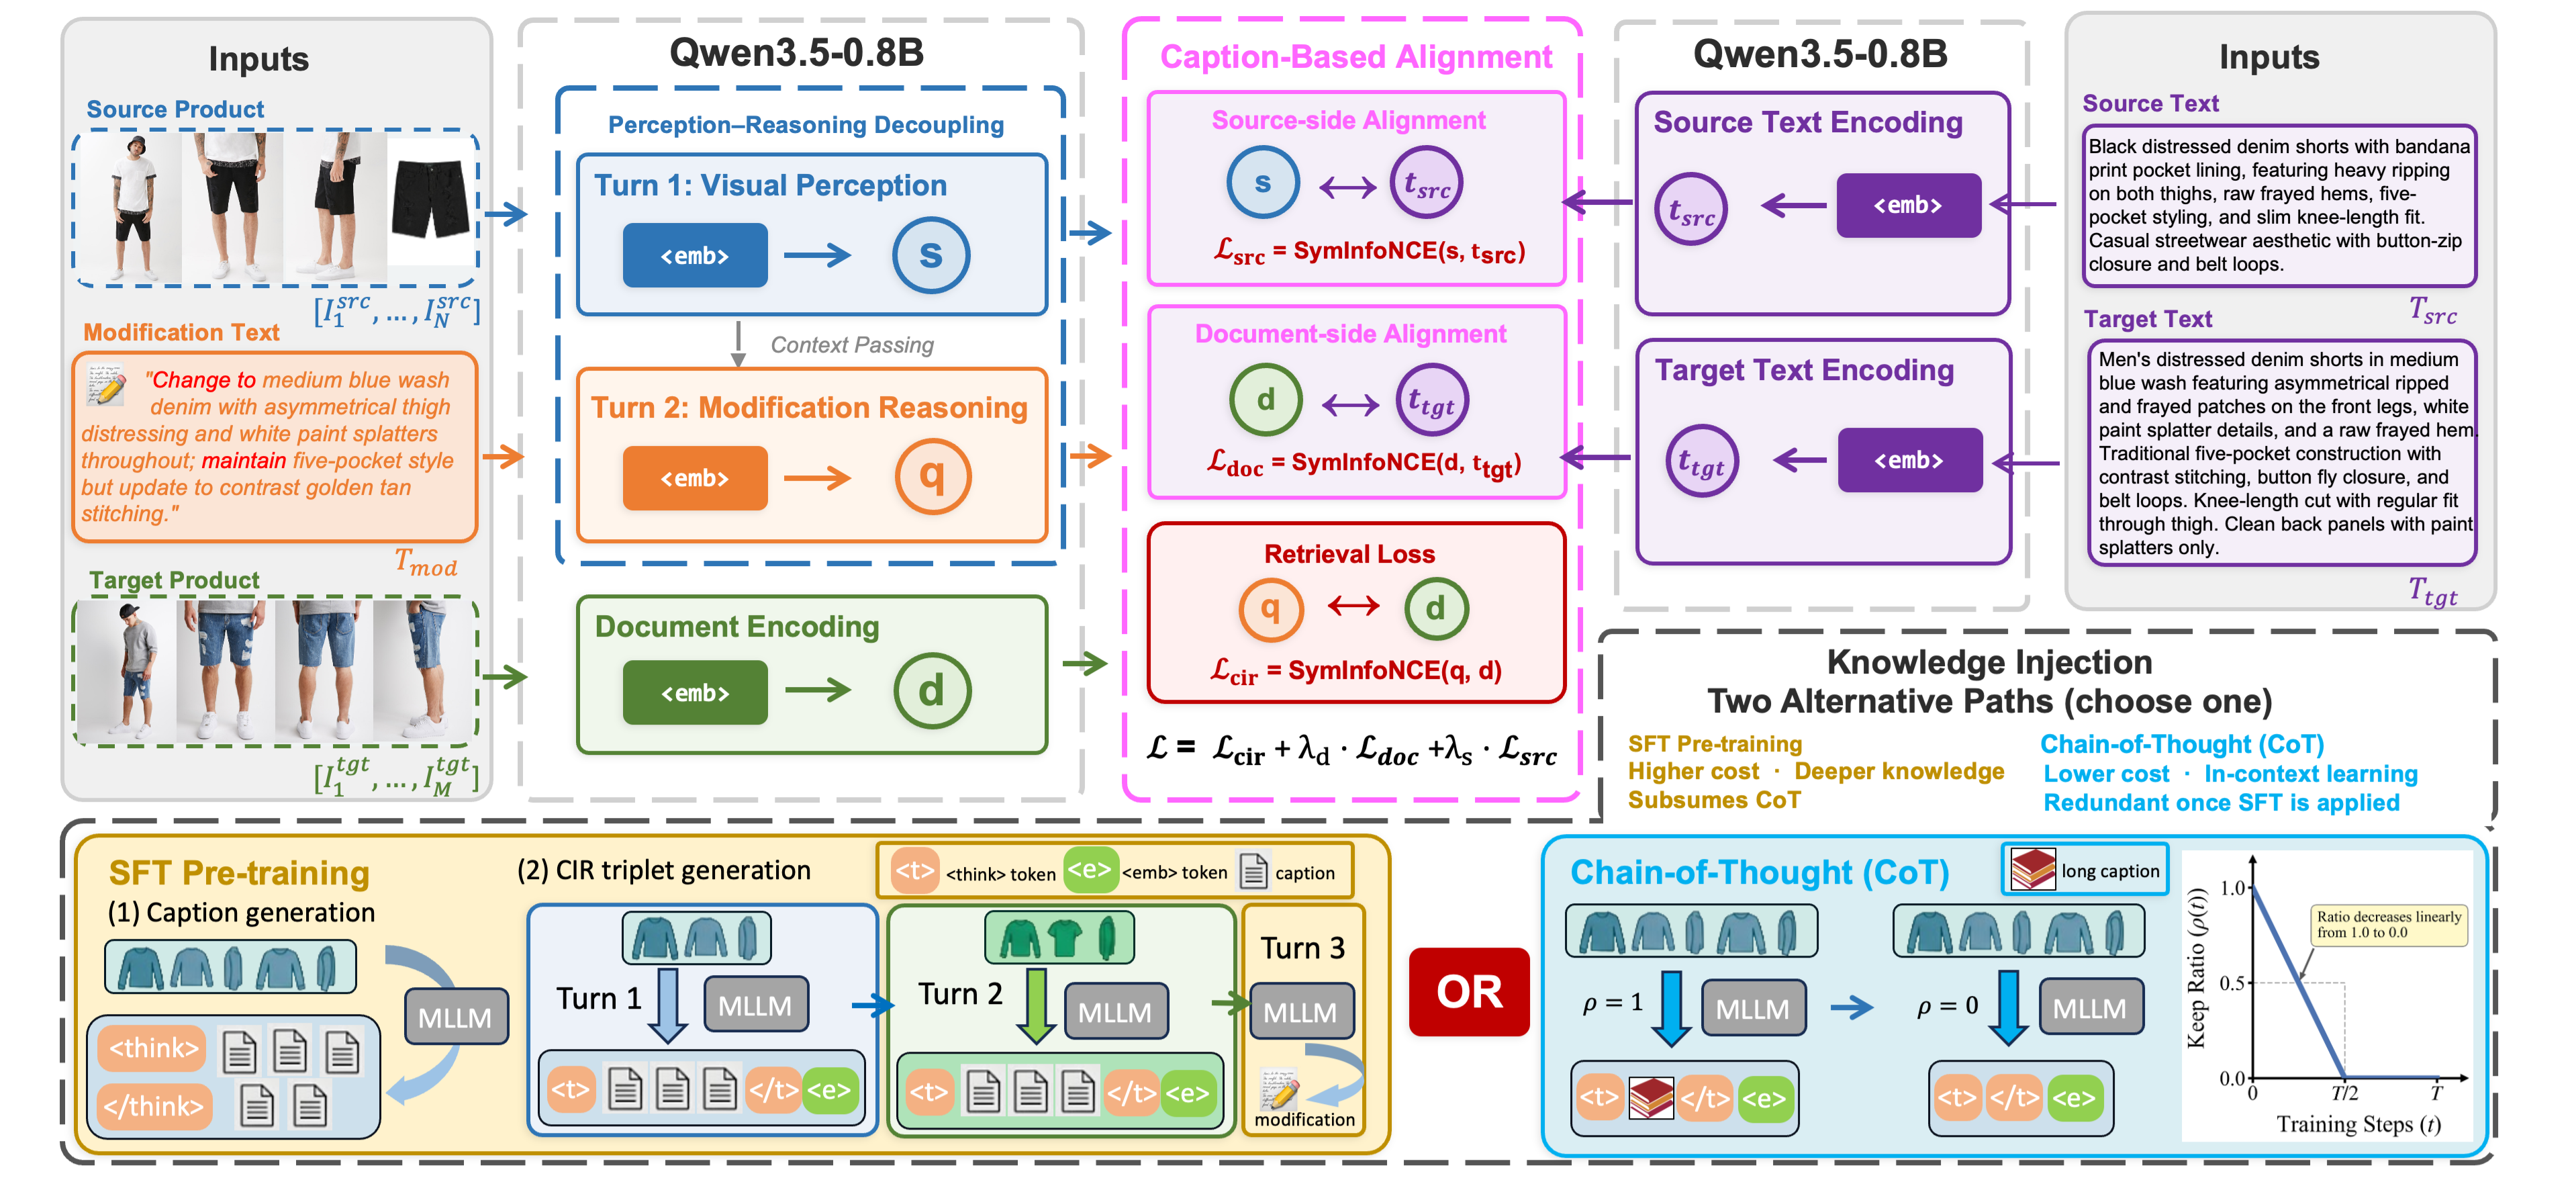
\includegraphics[width=\textwidth]{model_framework.png}
\caption{Kiến trúc huấn luyện ProCIR. Hội thoại hai lượt tách truy vấn thành Lượt 1 (nhận thức thị giác, tạo embedding nguồn $s$) và Lượt 2 (suy luận chỉnh sửa, tạo embedding truy vấn $q$); bộ mã hoá tài liệu tạo embedding đích $d$; căn chỉnh dựa trên chú thích kết nối $s$ và $d$ với embedding chú thích tương ứng (nguồn: Hình 3 trong~\cite{yuan2026fashionmv}).}
\label{fig:model_framework}
\end{figure}

\section{Xây dựng bộ dữ liệu FashionMV}\label{sec:dataset-construction}

\begin{figure}[h]
\centering
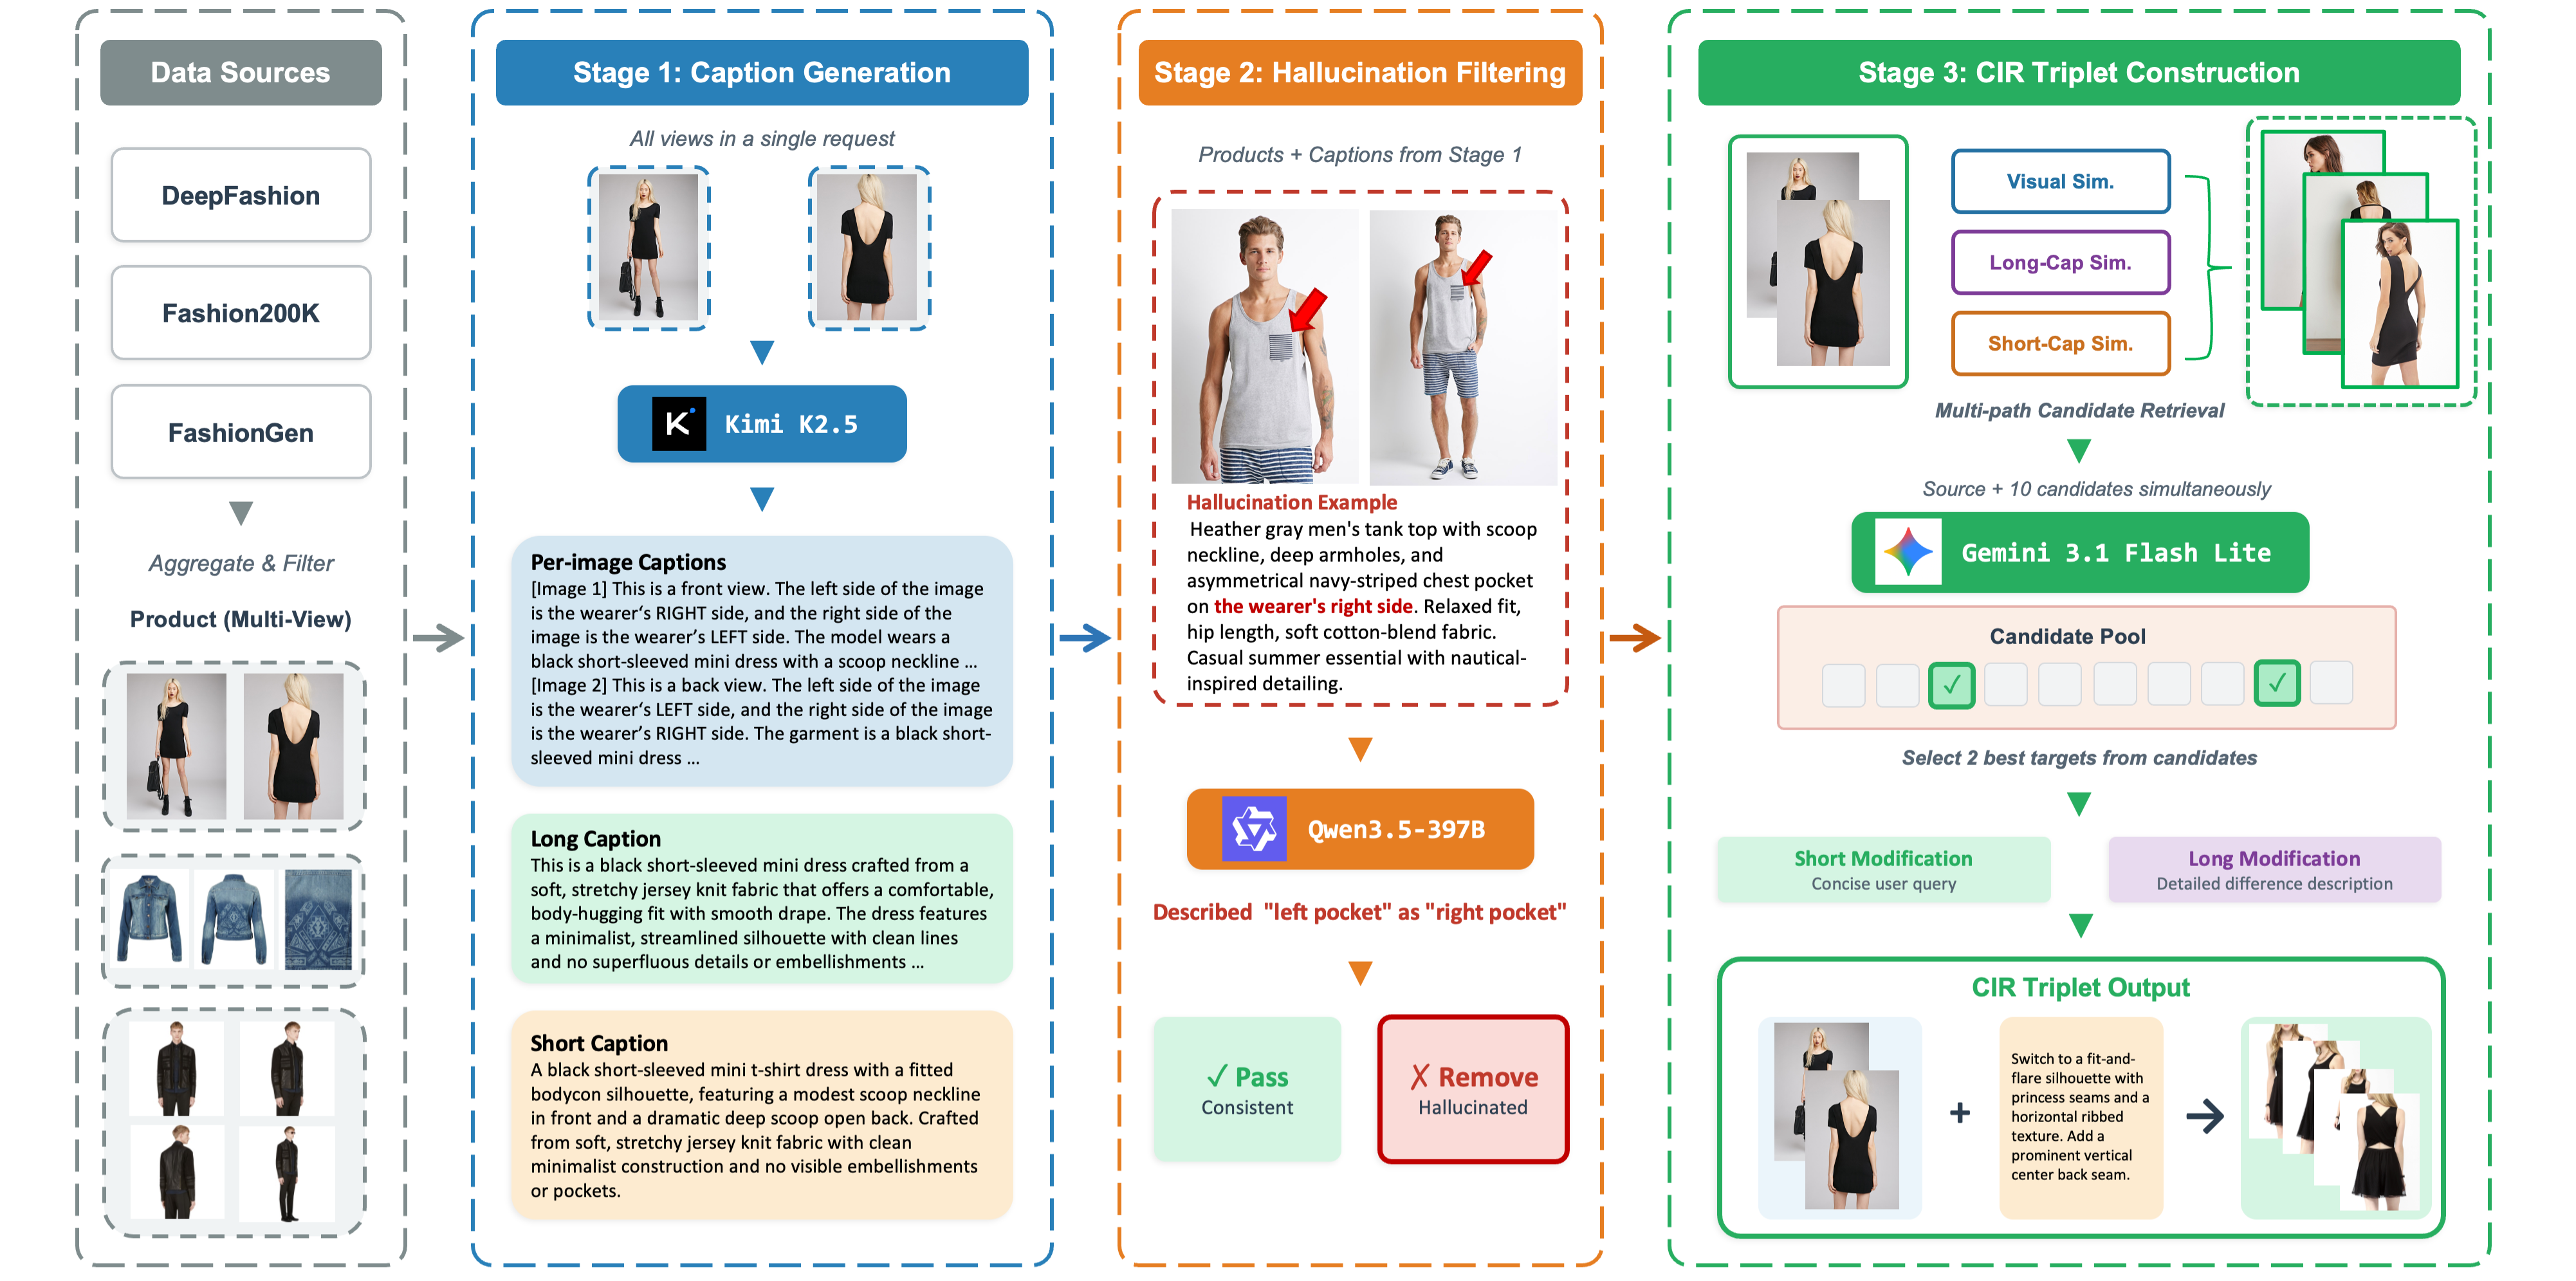
\includegraphics[width=\textwidth]{data_pipeline.png}
\caption{Pipeline ba giai đoạn xây dựng FashionMV. Giai đoạn 1: Kimi K2.5 sinh chú thích từ toàn bộ ảnh đa góc nhìn trong một yêu cầu. Giai đoạn 2: Qwen3.5-397B đối chiếu mô tả định hướng với bằng chứng thị giác và loại các sản phẩm có ảo giác. Giai đoạn 3: truy xuất đa đường tạo tập ứng viên; Gemini 3.1 Flash-Lite chọn tối đa 2 đích trong 10 ứng viên và sinh văn bản chỉnh sửa (nguồn: Hình 2 trong~\cite{yuan2026fashionmv}).}
\label{fig:data_pipeline}
\end{figure}

\subsection{Nguồn dữ liệu}

FashionMV tổng hợp sản phẩm từ ba bộ dữ liệu thời trang công khai, mỗi sản phẩm có từ 2 đến 5 ảnh chụp từ các góc nhìn khác nhau: DeepFashion (tác vụ In-shop Clothes Retrieval)~\cite{liu2016deepfashion}, Fashion200K~\cite{han2017fashion200k} và FashionGen~\cite{rostamzadeh2018fashiongen} (cả tập train và validation). Sau khi lọc bỏ các mục không phải trang phục, tập thô gồm 144.396 sản phẩm với khoảng 535 nghìn ảnh. Chi tiết về ba bộ dữ liệu nguồn được trình bày ở Mục~\ref{sec:datasets}.

\subsection{Giai đoạn 1: Sinh chú thích đa góc nhìn}

Với mỗi sản phẩm, toàn bộ ảnh đa góc nhìn được đưa vào mô hình Kimi K2.5~\cite{bai2026kimi} \emph{trong một yêu cầu duy nhất}, kèm nhãn số thứ tự ảnh. Mô hình sinh ra ba loại chú thích:
\begin{itemize}
    \item \textbf{Chú thích theo từng ảnh} (50--200 từ, trung vị 115 từ): xác định góc nhìn của ảnh (trước, sau, nghiêng, chi tiết\ldots) và các chi tiết đặc thù quan sát được từ góc nhìn đó.
    \item \textbf{Chú thích dài} (200--400 từ, trung vị 222 từ): tổng hợp mọi góc nhìn thành một mô tả sản phẩm toàn diện.
    \item \textbf{Chú thích ngắn} ($\sim$50 từ, trung vị 40 từ): nêu bật loại trang phục, phong cách, màu sắc và các đặc trưng phân biệt.
\end{itemize}
Việc đưa mọi góc nhìn vào cùng một yêu cầu cho phép mô hình đối chiếu xuyên góc nhìn ngay khi mô tả. Các chú thích này về sau đóng vai trò tín hiệu giám sát cho cơ chế căn chỉnh (Mục~\ref{sec:procir-align}), CoT (Mục~\ref{sec:procir-cot}) và SFT (Mục~\ref{sec:procir-sft}).

\subsection{Giai đoạn 2: Lọc ảo giác định hướng}

Mô tả ảnh thời trang đa góc nhìn đòi hỏi suy luận định hướng trái--phải chính xác: ``bên trái của ảnh'' ở góc nhìn trước tương ứng với ``bên phải của người mặc''. Tác giả phát hiện Kimi K2.5 đôi khi tạo ảo giác ở các mô tả định hướng, đặc biệt với các đặc trưng bất đối xứng như túi ngực đơn hay logo lệch tâm.

\paragraph{Đánh giá của con người.} Trên 1.000 sản phẩm lấy mẫu ngẫu nhiên và gán nhãn thủ công, 6,2\% chứa ảo giác nghiêm trọng, gồm lỗi trái--phải (5,0\%) và các lỗi mô tả lớn khác (1,2\%). Lỗi trái--phải chiếm hơn 80\% tổng số ảo giác nghiêm trọng.

\paragraph{Lọc tự động.} Qwen3.5-397B-A17B được dùng làm bộ kiểm chứng xuyên góc nhìn, kiểm tra mô tả định hướng có nhất quán với bằng chứng thị giác hay không. Trên tập gán nhãn thủ công, bộ phát hiện đạt precision 42,9\% và recall 36,0\% đối với lỗi trái--phải. Các sản phẩm có lỗi được xác nhận bị loại bỏ (Bảng~\ref{tab:hallucination}): tổng cộng 6.307 sản phẩm (4,37\%) bị lọc, giữ lại 138.089 sản phẩm với 510.877 ảnh.

\begin{table}[h]
\centering
\caption{Kết quả lọc ảo giác định hướng theo từng bộ dữ liệu (Bảng 4 trong tài liệu bổ sung của~\cite{yuan2026fashionmv}).}
\label{tab:hallucination}
\begin{tabular}{lrrrr}
\toprule
Bộ dữ liệu & Đã kiểm tra & Lỗi & Giữ lại & Tỷ lệ lỗi \\
\midrule
DeepFashion      & 12.711 & 487   & 12.224 & 3,83\% \\
Fashion200K      & 77.106 & 3.607 & 73.499 & 4,68\% \\
FashionGen-train & 48.476 & 1.942 & 46.534 & 4,01\% \\
FashionGen-val   & 6.086  & 271   & 5.815  & 4,45\% \\
\midrule
\textbf{Tổng}    & \textbf{144.379} & \textbf{6.307} & \textbf{138.072} & \textbf{4,37\%} \\
\bottomrule
\end{tabular}
\end{table}

Có thể nhận xét rằng precision và recall của bộ lọc tự động đều dưới 50\%, nghĩa là phần lớn ảo giác trái--phải vẫn còn lại trong dữ liệu sau lọc, đồng thời một phần sản phẩm bị loại là không có lỗi. Tuy vậy, với tỷ lệ lỗi ban đầu thấp (5,0\%) và chi phí loại bỏ nhỏ (4,37\% sản phẩm), đây là một sự đánh đổi chấp nhận được cho một pipeline hoàn toàn tự động.

\subsection{Giai đoạn 3: Xây dựng triplet CIR}

Với mỗi sản phẩm nguồn, các ứng viên đích được truy xuất qua ba đường bổ trợ: tương đồng thị giác, tương đồng chú thích dài và tương đồng chú thích ngắn; hợp của top-20 kết quả mỗi đường tạo thành tập ứng viên. Sau đó, 10 ứng viên được lấy mẫu ngẫu nhiên và trình bày cùng sản phẩm nguồn cho Gemini 3.1 Flash-Lite~\cite{google2026gemini}. Mô hình chọn tối đa 2 ứng viên tốt nhất theo ba tiêu chí: (i) sự khác biệt trải trên ít nhất hai góc nhìn; (ii) khả năng phân biệt rõ ràng; (iii) có chi tiết cấu trúc cụ thể. Với mỗi cặp được chọn, mô hình sinh:
\begin{itemize}
    \item một \textbf{văn bản chỉnh sửa ngắn} (16--32 từ, trung vị 23 từ), mô phỏng truy vấn súc tích người dùng thực tế nhập vào ô tìm kiếm -- được dùng để \emph{đánh giá};
    \item một \textbf{văn bản chỉnh sửa dài} (64--128 từ, trung vị 84 từ), mô tả chi tiết sự khác biệt -- cung cấp tín hiệu huấn luyện phong phú hơn.
\end{itemize}

\paragraph{So với gán nhãn theo cặp.} Các bộ dữ liệu trước đây (dù do con người gán nhãn như FashionIQ hay sinh tự động như FACap) ghép mỗi sản phẩm nguồn với \emph{một} sản phẩm tương tự rồi sinh văn bản chỉnh sửa từ cặp cô lập này. Cách làm đó có hai hạn chế: không lọc được các cặp không tương thích về phạm trù (ví dụ áo khoác nam ghép với váy nữ), và văn bản sinh ra thường mô tả những điểm chung ở mức phạm trù, dẫn đến mơ hồ đa đáp án đúng. Bằng cách trình bày đồng thời 10 ứng viên, pipeline của FashionMV cho phép mô hình loại cặp không tương thích và tập trung mô tả những thuộc tính phân biệt đích với 9 đối thủ cạnh tranh. Hình~\ref{fig:triplet_examples} minh hoạ một triplet trong bộ dữ liệu.

\begin{figure}[h]
\centering
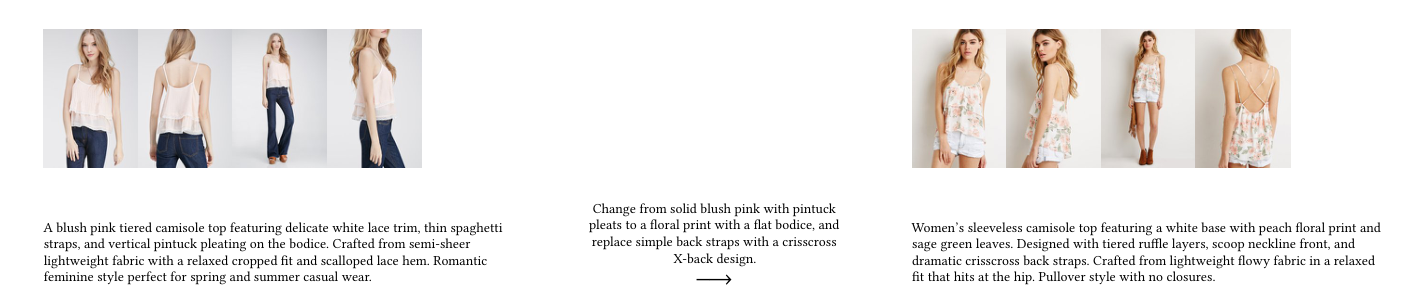
\includegraphics[width=\textwidth]{triplet_examples.png}
\caption{Ví dụ một triplet CIR trong FashionMV: sản phẩm nguồn (trái, 4 góc nhìn kèm chú thích ngắn), văn bản chỉnh sửa (giữa) và sản phẩm đích (phải). Văn bản chỉnh sửa đề cập đồng thời đến hoạ tiết mặt trước và dây đan chéo ở mặt sau (nguồn: Mục G, tài liệu bổ sung của~\cite{yuan2026fashionmv}).}
\label{fig:triplet_examples}
\end{figure}

Giai đoạn này tạo ra 220.733 triplet bao phủ 127.231 sản phẩm, trong đó 99,83\% triplet liên quan đến từ hai góc nhìn trở lên (Bảng~\ref{tab:view-comb}).

\begin{table}[h]
\centering
\caption{Phân bố tổ hợp góc nhìn được văn bản chỉnh sửa đề cập (Bảng 6 trong tài liệu bổ sung của~\cite{yuan2026fashionmv}).}
\label{tab:view-comb}
\begin{tabular}{lrr}
\toprule
Tổ hợp góc nhìn & Số triplet & Tỷ lệ \\
\midrule
sau + trước              & 180.040 & 81,6\% \\
trước + nghiêng          & 27.556  & 12,5\% \\
sau + trước + nghiêng    & 6.390   & 2,9\% \\
sau + nghiêng            & 4.636   & 2,1\% \\
sau + chi tiết + trước   & 416     & 0,2\% \\
Tổ hợp khác              & 1.695   & 0,8\% \\
\midrule
\textbf{Tổng}            & \textbf{220.733} & \textbf{100\%} \\
\bottomrule
\end{tabular}
\end{table}

\subsection{Phân chia và thống kê bộ dữ liệu}

Sản phẩm được chia thành tập huấn luyện và validation ở mức sản phẩm, không chồng lấn. FashionGen giữ phân chia gốc; DeepFashion và Fashion200K được chia ngẫu nhiên. Triplet được xây dựng độc lập trong từng phân vùng -- truy xuất lân cận, chọn ứng viên và sinh văn bản đều diễn ra trong cùng một phân vùng -- cho ra 188.015 triplet huấn luyện và 32.718 triplet validation (Bảng~\ref{tab:splits}). Hình~\ref{fig:views_distribution} cho thấy phân bố số góc nhìn mỗi sản phẩm khác nhau rõ rệt giữa các bộ: phần lớn sản phẩm FashionGen có 4 góc nhìn, DeepFashion tập trung ở 4 góc nhìn, còn Fashion200K trải đều từ 2 đến 5 với nhiều sản phẩm chỉ có 2--3 ảnh.

\begin{table}[h]
\centering
\caption{Phân chia triplet và sản phẩm của FashionMV~\cite{yuan2026fashionmv}.}
\label{tab:splits}
\begin{tabular}{lrrrr}
\toprule
Bộ dữ liệu & Triplet train & Triplet val & Sản phẩm train & Sản phẩm val \\
\midrule
DeepFashion   & 16.399 & 5.188  & 8.856  & 2.791 \\
Fashion200K   & 98.800 & 18.499 & 56.960 & 10.720 \\
FashionGen    & 72.816 & 9.031  & 42.612 & 5.292 \\
\midrule
\textbf{Tổng} & \textbf{188.015} & \textbf{32.718} & \textbf{108.428} & \textbf{18.803} \\
\bottomrule
\end{tabular}
\end{table}

\begin{figure}[h]
\centering
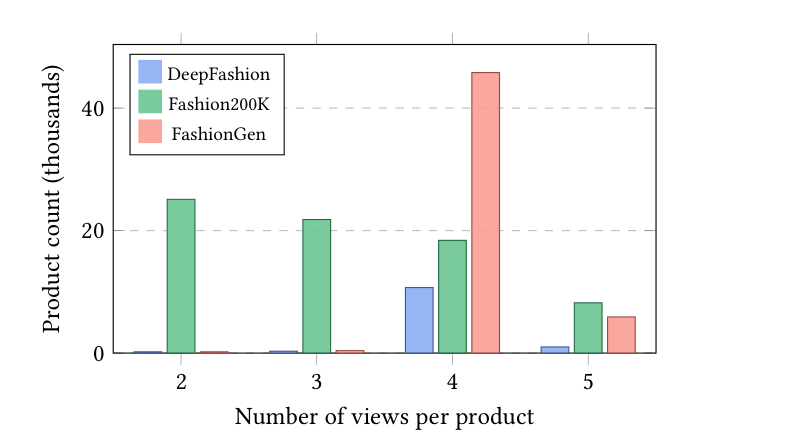
\includegraphics[width=0.62\textwidth]{views_distribution.png}
\caption{Phân bố số góc nhìn mỗi sản phẩm theo từng bộ dữ liệu con (nguồn: Hình 4 trong tài liệu bổ sung của~\cite{yuan2026fashionmv}).}
\label{fig:views_distribution}
\end{figure}

\section{Trích xuất embedding từ MLLM}\label{sec:procir-embedding}

ProCIR sử dụng Qwen3.5-0.8B (Bảng~\ref{tab:qwen35-config}) làm xương sống. Để trích xuất embedding có chiều cố định, một token đặc biệt \texttt{<emb>} được thêm vào từ vựng (trong mã nguồn công bố là \texttt{<emb\_all>}) và gắn vào cuối mỗi lượt trả lời của assistant. Trạng thái ẩn ở tầng cuối tại vị trí này là embedding mức sản phẩm:
\begin{equation}
    \mathbf{e} = h_{LLM}[\texttt{<emb>}] \in \mathbb{R}^{d}, \qquad d = 1024.
    \label{eq:emb}
\end{equation}
Mọi ảnh đa góc nhìn được đưa vào như token thị giác trong cùng một yêu cầu; attention nhân quả của mô hình tự nhiên tổng hợp thông tin xuyên góc nhìn mà không cần phép gộp (pooling) tường minh -- tương ứng với chiến lược mã hoá \emph{Joint}. Mỗi lượt assistant luôn có một khối \texttt{<think>...</think>}, để trống khi không dùng CoT. Phía tài liệu (gallery), sản phẩm đích được mã hoá chỉ bằng ảnh, không có văn bản:
\begin{equation}
    [I^{tgt}_1, \dots, I^{tgt}_M] \;\to\; \mathbf{d}.
\end{equation}

\section{Biến thể cơ sở: CIR một lượt hội thoại}

Biến thể cơ sở của ProCIR xử lý truy vấn trong một lượt duy nhất: ảnh nguồn và văn bản chỉnh sửa được nối trong cùng một tin nhắn người dùng,
\begin{equation}
    \underbrace{[I^{src}_1, \dots, I^{src}_N]}_{\text{ảnh đa góc nhìn}} \oplus T_{mod} \;\to\; \mathbf{q},
\end{equation}
và được huấn luyện bằng hàm SymInfoNCE~\eqref{eq:syminfonce} giữa $\mathbf{q}$ và $\mathbf{d}$:
\begin{equation}
    \mathcal{L}_{cir} = \mathrm{SymInfoNCE}(\mathbf{q}, \mathbf{d}, \tau), \qquad \tau = 0{,}07,
\end{equation}
với mẫu âm là mọi mẫu khác trong batch, tập hợp xuyên GPU bằng all-gather. Khi huấn luyện, văn bản chỉnh sửa được lấy mẫu ngẫu nhiên từ phiên bản dài hoặc ngắn với xác suất bằng nhau; khi đánh giá chỉ dùng phiên bản ngắn.

\section{Kiến trúc hội thoại hai lượt}\label{sec:two-stage}

Biến thể một lượt gộp lẫn nhận thức thị giác và suy luận chỉnh sửa trong một lần truyền xuôi: văn bản chỉnh sửa có thể cạnh tranh với nội dung thị giác để giành attention, và embedding truy vấn là hỗn hợp đặc trưng thị giác--văn bản, khiến không thể căn chỉnh riêng phần thị giác của sản phẩm nguồn với chú thích của nó. ProCIR giải quyết bằng cách tách truy vấn thành hai lượt hội thoại:
\begin{align}
    \text{Lượt 1 (Nhận thức):} &\quad [I^{src}_1, \dots, I^{src}_N] \;\to\; \mathbf{s}, \\
    \text{Lượt 2 (Suy luận):}  &\quad T_{mod} \;\to\; \mathbf{q}.
\end{align}
Hình~\ref{fig:two-stage-seq} minh hoạ chuỗi token thực tế của một truy vấn hai lượt, được dựng lại từ lớp \texttt{CIRQueryCollator} trong mã nguồn đánh giá.

\begin{figure}[h]
\centering
\begin{tikzpicture}[
  seg/.style={draw, minimum height=0.75cm, font=\scriptsize, align=center, inner sep=2pt},
  arr/.style={-{Stealth[length=2mm]}, thick}
]
\node[seg, fill=gray!15, minimum width=1.2cm] (u1) at (0,0) {\texttt{user}};
\node[seg, fill=blue!20, minimum width=2.5cm, right=0pt of u1] (im) {$I^{src}_1 \cdots I^{src}_N$};
\node[seg, fill=gray!15, minimum width=1.7cm, right=0pt of im] (a1) {\texttt{assistant}\\[-2pt]\tiny\texttt{<think></think>}};
\node[seg, fill=red!35, minimum width=1.0cm, right=0pt of a1] (e1) {\texttt{<emb>}};
\node[seg, fill=gray!15, minimum width=1.2cm, right=0pt of e1] (u2) {\texttt{user}};
\node[seg, fill=orange!25, minimum width=2.2cm, right=0pt of u2] (tm) {$T_{mod}$ (ngắn)};
\node[seg, fill=gray!15, minimum width=1.7cm, right=0pt of tm] (a2) {\texttt{assistant}\\[-2pt]\tiny\texttt{<think></think>}};
\node[seg, fill=red!35, minimum width=1.0cm, right=0pt of a2] (e2) {\texttt{<emb>}};
\draw[decorate, decoration={brace, amplitude=5pt}] (u1.north west) -- (e1.north east) node[midway, above=6pt, font=\scriptsize\bfseries] {Lượt 1 -- Nhận thức};
\draw[decorate, decoration={brace, amplitude=5pt}] (u2.north west) -- (e2.north east) node[midway, above=6pt, font=\scriptsize\bfseries] {Lượt 2 -- Suy luận};
\draw[arr] (e1.south) -- ++(0,-0.6) node[below, font=\scriptsize] {$\mathbf{s}$: chỉ thấy ảnh};
\draw[arr] (e2.south) -- ++(0,-0.6) node[below, font=\scriptsize] {$\mathbf{q}$: thấy toàn bộ ngữ cảnh};
\end{tikzpicture}
\caption{Chuỗi token của một truy vấn hai lượt trong ProCIR. Do attention nhân quả, $\mathbf{s}$ tại \texttt{<emb>} thứ nhất không bị ảnh hưởng bởi văn bản chỉnh sửa; $\mathbf{q}$ tại \texttt{<emb>} thứ hai tổng hợp cả ảnh nguồn lẫn văn bản.}
\label{fig:two-stage-seq}
\end{figure}

Lượt 1 chỉ xử lý ảnh nguồn và tạo embedding nguồn $\mathbf{s}$ tại \texttt{<emb>} thứ nhất. Lượt 2 nhận văn bản chỉnh sửa và tạo embedding truy vấn $\mathbf{q}$ tại \texttt{<emb>} thứ hai. Thiết kế này mang lại bốn lợi ích:
\begin{enumerate}
    \item $\mathbf{s}$ là một biểu diễn \emph{thị giác thuần tuý} của sản phẩm nguồn;
    \item nhờ đó có thể căn chỉnh $\mathbf{s}$ với chú thích của sản phẩm nguồn (Mục~\ref{sec:procir-align}) -- điều không thể làm với biến thể một lượt;
    \item $\mathbf{s}$ là sản phẩm phụ ``miễn phí'', có cùng không gian với embedding gallery $\mathbf{d}$, cho phép dùng chính sản phẩm nguồn làm mục trong gallery mà không cần mã hoá thêm -- mã đánh giá công khai thực sự tận dụng điều này khi bổ sung các sản phẩm nguồn chưa có vào gallery;
    \item trạng thái key--value của Lượt 1 có thể tính trước và lưu cache trước khi người dùng nhập văn bản chỉnh sửa, nên Lượt 2 chỉ cần suy luận gia tăng trên vài chục token -- hữu ích cho truy xuất tương tác độ trễ thấp.
\end{enumerate}

\section{Căn chỉnh dựa trên chú thích}\label{sec:procir-align}

Để tiêm ngữ nghĩa sản phẩm vào không gian embedding, mỗi chú thích (dài hoặc ngắn, chọn ngẫu nhiên với xác suất bằng nhau ở mỗi bước) được mã hoá qua một lượt truyền xuôi chỉ có văn bản:
\begin{equation}
    \mathbf{t}_{cap} = h_{LLM}[T_{cap};\, \texttt{<emb>}] \in \mathbb{R}^{d}.
\end{equation}
Ở phía tài liệu, embedding thị giác của sản phẩm đích được căn chỉnh với chú thích của chính nó:
\begin{equation}
    \mathcal{L}_{doc} = \mathrm{SymInfoNCE}(\mathbf{d}, \mathbf{t}_{tgt}, \tau).
\end{equation}
Với các biến thể hai lượt, embedding nguồn thuần thị giác $\mathbf{s}$ được căn chỉnh thêm với chú thích nguồn:
\begin{equation}
    \mathcal{L}_{src} = \mathrm{SymInfoNCE}(\mathbf{s}, \mathbf{t}_{src}, \tau).
\end{equation}
Trực giác của cơ chế này là: chú thích dài mô tả tường minh các chi tiết trên mọi góc nhìn (``dây đan chéo ở lưng'', ``túi ngực bên trái người mặc''); buộc embedding thị giác gần với embedding của mô tả đó sẽ khuyến khích mô hình mã hoá chính những chi tiết này -- vốn là những gì văn bản chỉnh sửa thường đề cập. Đồng thời, việc đưa embedding thị giác và văn bản về cùng không gian giúp $\mathbf{q}$ (được tạo sau khi đọc văn bản) dễ dàng ``di chuyển'' theo hướng văn bản chỉ định.

\section{Chuỗi suy luận với loại bỏ tiệm tiến}\label{sec:procir-cot}

Song song với căn chỉnh (tiêm tri thức qua một hàm mất mát phụ), bài báo khảo sát việc tiêm tri thức trực tiếp vào ngữ cảnh: chú thích dài của sản phẩm được đặt bên trong khối suy luận,
\begin{center}
\texttt{assistant: <think>\{chú thích dài (lấy mẫu con)\}</think> <emb>},
\end{center}
để mô hình ``đọc'' mô tả sản phẩm trước khi tạo embedding. CoT được áp dụng cho phía tài liệu và cho Lượt 1 của truy vấn; Lượt 2 không dùng CoT. Để tránh mô hình phụ thuộc vào chú thích -- vốn không có sẵn khi suy luận -- một tỷ lệ giữ lại $\rho(t)$ kiểm soát phần trăm token chú thích được giữ:
\begin{equation}
    \rho(t) = \max\!\left(0,\; 1 - \frac{t}{0{,}5\,T}\right),
\end{equation}
với $T$ là tổng số bước huấn luyện. $\rho$ giảm tuyến tính từ 1 về 0 trong nửa đầu quá trình huấn luyện; tại mỗi bước giữ ngẫu nhiên $\lceil \rho \cdot |\text{tokens}| \rceil$ token. Như vậy, mô hình được chuyển dần từ trạng thái có đầy đủ chú thích sang chế độ suy luận không chú thích, với kỳ vọng nội hoá được tri thức ngữ nghĩa.

\section{Hàm mục tiêu huấn luyện}\label{sec:procir-objective}

Hàm mục tiêu đầy đủ kết hợp ba thành phần:
\begin{equation}
    \mathcal{L} = \mathcal{L}_{cir} + \lambda_d\,\mathcal{L}_{doc} + \lambda_s\,\mathcal{L}_{src}, \qquad \lambda_d = \lambda_s = 0{,}25,
    \label{eq:procir-loss}
\end{equation}
trong đó $\mathcal{L}_{doc}$ và $\mathcal{L}_{src}$ chỉ được kích hoạt ở các biến thể có Align, và $\mathcal{L}_{src}$ chỉ tồn tại ở biến thể hai lượt (vì cần $\mathbf{s}$). Tổ hợp ba công tắc MT, Align, CoT cho ra 8 biến thể.

\section{Tinh chỉnh có giám sát}\label{sec:procir-sft}

Trước huấn luyện tương phản, Qwen3.5-0.8B có thể được tinh chỉnh có giám sát trên hai loại dữ liệu từ tập huấn luyện FashionMV:
\begin{enumerate}
    \item \textbf{Sinh chú thích}: hội thoại một lượt, người dùng cung cấp mọi ảnh đa góc nhìn, assistant sinh chú thích theo từng ảnh trong khối \texttt{<think>} rồi đến một đối tượng JSON chứa chú thích dài và ngắn -- dạy mô hình nhận diện góc nhìn, trích thuộc tính và tổng hợp xuyên góc nhìn.
    \item \textbf{Sinh triplet CIR}: hội thoại ba lượt -- Lượt 1 với ảnh nguồn (sinh chú thích nguồn, sau đó \texttt{<emb>}), Lượt 2 với ảnh đích (tương tự), Lượt 3 sinh văn bản chỉnh sửa dạng JSON -- giúp mô hình làm quen với suy luận đa lượt và ngữ nghĩa của token embedding.
\end{enumerate}
Bài báo lấy ngẫu nhiên 20\% dữ liệu khả dụng (117.610 mẫu sinh chú thích và 187.940 mẫu sinh triplet, tổng 305.550 mẫu) và huấn luyện toàn bộ mô hình trong một epoch với hàm mất mát tự hồi quy chuẩn trên các token của assistant:
\begin{equation}
    \mathcal{L}_{sft} = -\sum_{t \in \mathcal{A}} \log p_\theta(x_t \mid x_{<t}).
\end{equation}
Checkpoint SFT được dùng làm khởi tạo thay thế cho cả 8 biến thể, tạo thành tổng cộng 16 cấu hình thực nghiệm.

\section{Kết quả thực nghiệm trong bài báo gốc}\label{sec:paper-results}

\subsection{Thiết lập}

Mọi biến thể được huấn luyện một epoch trên 188 nghìn triplet với AdamW~\cite{loshchilov2019adamw} (tốc độ học $10^{-5}$, weight decay 0,01, lịch cosine không warmup), gradient clipping 1,0, độ chính xác bfloat16, batch 16 mỗi GPU trên 10 GPU RTX 3090 (batch hiệu dụng 160, tổng 1.175 bước). Ảnh được giới hạn trong khoảng $128^2$--$512^2$ điểm ảnh, tối đa 5 góc nhìn mỗi sản phẩm. Đánh giá thực hiện độc lập trên ba bộ: DeepFashion (DF), Fashion200K (F200K) và FashionGen-val (FG), mỗi bộ có gallery riêng gồm các sản phẩm validation của nó, chỉ dùng văn bản chỉnh sửa ngắn, báo cáo Recall@5 và Recall@10.

\subsection{So sánh với các mô hình hiện có}

Vì chưa có phương pháp nào giải quyết trực tiếp Multi-View CIR, tác giả thích nghi các mô hình embedding tiêu biểu bằng ba chiến lược mã hoá đa góc nhìn. Gọi $\{\mathbf{e}_1, \dots, \mathbf{e}_N\}$ là các embedding theo từng góc nhìn:
\begin{align}
    s_{\mathrm{Joint}}(Q, D) &= \cos\big(\mathbf{e}^Q_{prod}, \mathbf{e}^D_{prod}\big), \\
    s_{\mathrm{MeanPool}}(Q, D) &= \cos\Big(\tfrac{1}{N_Q}\textstyle\sum_i \mathbf{e}^Q_i,\; \tfrac{1}{N_D}\sum_j \mathbf{e}^D_j\Big), \\
    s_{\mathrm{MaxSim}}(Q, D) &= \max_{i \in [N_Q],\, j \in [N_D]} \cos\big(\mathbf{e}^Q_i, \mathbf{e}^D_j\big),
\end{align}
trong đó Joint đưa mọi góc nhìn vào mô hình đồng thời (đòi hỏi mô hình hỗ trợ đa ảnh nguyên bản). Kết quả được tóm tắt ở Bảng~\ref{tab:paper-comparison}.

\begin{table}[h]
\centering
\caption{So sánh với các mô hình hiện có trên tập validation FashionMV (trích Bảng 2 của~\cite{yuan2026fashionmv}; với mỗi mô hình chỉ giữ chiến lược mã hoá có điểm trung bình tốt nhất).}
\label{tab:paper-comparison}
\small
\begin{tabular}{llcccccccc}
\toprule
& & \multicolumn{2}{c}{DeepFashion} & \multicolumn{2}{c}{F200K} & \multicolumn{2}{c}{FashionGen} & \multicolumn{2}{c}{Trung bình} \\
\cmidrule(lr){3-4}\cmidrule(lr){5-6}\cmidrule(lr){7-8}\cmidrule(lr){9-10}
Mô hình (tham số) & Mã hoá & R@5 & R@10 & R@5 & R@10 & R@5 & R@10 & R@5 & R@10 \\
\midrule
CLIP4Cir (0,25B)   & MeanPool & 28,0 & 39,3 & 13,3 & 19,3 & 16,2 & 23,6 & 19,2 & 27,4 \\
SPRC (1,2B)        & MaxSim   & 55,8 & 67,7 & 34,4 & 43,7 & 42,7 & 53,0 & 44,3 & 54,8 \\
RzenEmbed (8B)     & MeanPool & 47,5 & 58,0 & 28,0 & 36,5 & 32,5 & 42,2 & 36,0 & 45,6 \\
Doubao-E-V (--)    & MaxSim   & 82,3 & 90,8 & 62,2 & 72,6 & 67,2 & 77,1 & 70,6 & 80,2 \\
Qwen3-V-2B (2B)    & Joint    & 75,7 & 86,4 & 61,1 & 72,3 & 63,0 & 74,1 & 66,6 & 77,6 \\
Qwen3-V-8B (8B)    & Joint    & 87,4 & 93,2 & 73,8 & 82,1 & 74,7 & 83,5 & 78,6 & 86,3 \\
\midrule
\textbf{ProCIR (0,8B)} & Joint & \textbf{89,2} & \textbf{94,9} & \textbf{77,6} & \textbf{86,6} & \textbf{75,0} & \textbf{85,3} & \textbf{80,6} & \textbf{88,9} \\
\bottomrule
\end{tabular}
\end{table}

Mô hình 0,8B của bài báo vượt mọi baseline trên mọi bộ dữ liệu, kể cả Qwen3-VL-Embedding 8B lớn hơn 10 lần (cao hơn +1,8/+3,8/+0,3 điểm R@5 trên DF/F200K/FG khi cùng dùng Joint). Các phương pháp CIR một-ảnh (CLIP4Cir, SPRC) kém hơn rõ rệt, cho thấy kiến trúc thiết kế cho truy vấn một ảnh không đủ cho truy xuất sản phẩm đa góc nhìn. Một phát hiện đáng chú ý khác là: với các mô hình hiểu đa ảnh tốt (Qwen3-V-8B), Joint vượt cả MeanPool và MaxSim; nhưng với các mô hình yếu hơn, xu hướng đảo ngược -- Joint của RzenEmbed (18,6 R@5 trung bình) chỉ bằng khoảng một nửa MeanPool (36,0), và Joint của Doubao-E-V (58,0) cũng kém MeanPool (68,3) và MaxSim (70,6). Điều này cho thấy mã hoá đồng thời nhiều góc nhìn không phải lúc nào cũng có lợi, mà phụ thuộc vào năng lực hiểu đa ảnh của mô hình.

\subsection{Kết quả ablation}

Bảng~\ref{tab:ablation} trình bày đầy đủ 16 cấu hình. Thứ tự các hàng được học viên đối chiếu lại với các phép tính chênh lệch nêu trong văn bản bài báo (ví dụ ``thêm Align vào MT+CoT cho +11,8/+9,5/+13,3 điểm R@5'') để xác định tổ hợp cơ chế của từng hàng.

\begin{table}[h]
\centering
\caption{Kết quả ablation trên tập validation (R@5 / R@10, trích Bảng 3 của~\cite{yuan2026fashionmv}). Thời gian huấn luyện trên 10$\times$RTX 3090; các hàng SFT đã bao gồm 4 giờ 29 phút tiền huấn luyện SFT. In đậm: tốt nhất trong nhóm.}
\label{tab:ablation}
\small
\begin{tabular}{cccccccr}
\toprule
MT & Align & CoT & DeepFashion & F200K & FashionGen & TB R@5 & Thời gian \\
\midrule
\multicolumn{8}{l}{\emph{Khởi tạo Pretrained}} \\
   &       &     & 77,0 / 87,8 & 61,4 / 73,6 & 59,7 / 72,5 & 66,0 & 7h25m \\
   & \tick &     & 78,7 / 88,7 & 61,5 / 74,1 & 62,6 / 74,5 & 67,6 & 8h13m \\
   &       & \tick & 77,9 / 87,9 & 60,5 / 71,6 & 56,3 / 68,6 & 64,9 & 8h31m \\
   & \tick & \tick & 77,5 / 87,4 & 61,8 / 73,1 & 57,4 / 69,6 & 65,6 & 9h20m \\
\tick &    &     & 77,8 / 88,3 & 60,7 / 73,0 & 59,4 / 72,3 & 66,0 & 7h20m \\
\tick & \tick &  & 79,5 / 89,0 & 61,8 / 73,8 & 62,7 / 74,9 & 68,0 & 8h53m \\
\tick &    & \tick & 72,3 / 84,2 & 59,1 / 71,2 & 54,4 / 67,1 & 61,9 & 8h27m \\
\tick & \tick & \tick & \textbf{84,1 / 91,5} & \textbf{68,6 / 79,0} & \textbf{67,7 / 77,8} & \textbf{73,5} & 10h04m \\
\midrule
\multicolumn{8}{l}{\emph{Khởi tạo SFT}} \\
   &       &     & 84,5 / 92,7 & 69,5 / 81,7 & 65,5 / 78,4 & 73,2 & 11h54m \\
   & \tick &     & 88,2 / 94,2 & 76,8 / 86,1 & 74,5 / 84,5 & 79,8 & 12h42m \\
   &       & \tick & 83,4 / 91,1 & 68,1 / 78,2 & 62,4 / 73,2 & 71,3 & 13h00m \\
   & \tick & \tick & 83,7 / 91,3 & 69,1 / 78,9 & 63,8 / 74,7 & 72,2 & 13h49m \\
\tick &    &     & 82,7 / 92,3 & 68,2 / 81,0 & 65,6 / 78,7 & 72,2 & 11h49m \\
\tick & \tick &  & \textbf{89,2 / 94,9} & \textbf{77,6 / 86,6} & \textbf{75,0 / 85,3} & \textbf{80,6} & 13h22m \\
\tick &    & \tick & 83,4 / 91,4 & 70,1 / 80,0 & 67,0 / 77,6 & 73,5 & 12h56m \\
\tick & \tick & \tick & 88,2 / 94,0 & 75,6 / 84,3 & 73,3 / 82,4 & 79,0 & 14h33m \\
\bottomrule
\end{tabular}
\end{table}

Bài báo rút ra ba phát hiện chính:

\paragraph{Phát hiện 1: MT + Align + CoT tối đa hoá việc tiêm tri thức khi không có SFT.} Trong nhóm Pretrained, tổ hợp đủ ba cơ chế đạt kết quả tốt nhất trên mọi bộ (R@5 trung bình 73,5), vượt xa các biến thể thiếu bất kỳ cơ chế nào. Ba cơ chế bổ trợ nhau: MT tách nhận thức khỏi suy luận và mở đường cho căn chỉnh phía nguồn; Align neo giữ không gian thị giác--văn bản; CoT tiêm chú thích vào quá trình suy luận.

\paragraph{Phát hiện 2: Căn chỉnh là cơ chế đơn lẻ quan trọng nhất.} Thêm Align vào MT+CoT (nhóm Pretrained) mang lại +11,8/+9,5/+13,3 điểm R@5 trên DF/F200K/FG. Ngược lại, \emph{không có} Align, kiến trúc hai lượt còn kém biến thể một lượt (R@5 72,3 so với 77,0 trên DF) -- tức là kiến trúc tách bạch chỉ phát huy tác dụng khi có neo giữ xuyên phương thức tường minh. CoT không kèm Align có tác động hạn chế hoặc thậm chí tiêu cực.

\paragraph{Phát hiện 3: CoT trở nên không cần thiết sau SFT.} Trong nhóm Pretrained, thêm CoT vào MT+Align tăng R@5 +4,6/+6,8/+5,0 điểm. Nhưng sau SFT, thêm CoT vào MT+Align lại \emph{giảm} $-1{,}0/-2{,}0/-1{,}7$ điểm. Cấu hình tốt nhất tổng thể là \textbf{MT+Align+SFT} (không CoT) -- chính là checkpoint được công bố và được tái lập trong báo cáo này. Điều này cho thấy SFT và CoT là hai con đường tiêm tri thức có chức năng chồng lấn.

\subsection{Phân tích bổ sung trong bài báo}

\paragraph{Độ khó của các bộ dữ liệu.} DeepFashion dễ nhất: gallery nhỏ nhất (2.791 sản phẩm) và ảnh độ phân giải cao ($>512 \times 512$). Fashion200K khó hơn do gallery lớn nhất (10.720 sản phẩm) và số góc nhìn trung bình thấp nhất ($\sim$3,3). FashionGen-val khó nhất do độ phân giải thấp ($256 \times 256$), dù có nhiều góc nhìn nhất ($\sim$4,1). Hai yếu tố \emph{kích thước gallery} và \emph{độ phân giải ảnh} được chính tác giả chỉ ra ở đây là hai yếu tố trung tâm trong phân tích sai lệch tái lập ở Chương~\ref{chapter:experiments}.

\paragraph{SFT cải thiện mọi biến thể.} Khởi tạo SFT tăng trung bình +8,5 điểm R@5 trên cả 8 biến thể và 3 bộ dữ liệu; biến thể cơ sở tăng +7,5/+8,1/+5,8 điểm. Tuy nhiên SFT đòi hỏi giám sát đa mức độ chi tiết (chú thích theo ảnh, chú thích sản phẩm, văn bản chỉnh sửa) -- vốn là sản phẩm phụ của pipeline dữ liệu -- và bản thân mô hình SFT không có khả năng tạo embedding; huấn luyện tương phản vẫn không thể thiếu.

\paragraph{Chi phí huấn luyện.} Biến thể nhanh nhất (chỉ MT) mất khoảng 7 giờ 20 phút, cấu hình đắt nhất (MT+Align+CoT+SFT) mất khoảng 14 giờ 33 phút trên 10 GPU RTX 3090. Chênh lệch đến từ số lần truyền xuôi mỗi bước: Align thêm một (phía tài liệu) hoặc hai (cả hai phía, khi có MT) lần truyền xuôi chỉ văn bản; CoT kéo dài chuỗi token.

\paragraph{Ví dụ định tính.} Hình~\ref{fig:retrieval_case} trích một ví dụ truy xuất trong tài liệu bổ sung của bài báo. Đáng chú ý, ở ví dụ này kết quả \#1 của ProCIR chính là \emph{sản phẩm nguồn}, và sản phẩm đích đúng đứng ở hạng 2. Quan sát này là điểm khởi đầu cho một phân tích về giao thức đánh giá được trình bày ở Mục~\ref{sec:source-in-gallery}.

\begin{figure}[h]
\centering
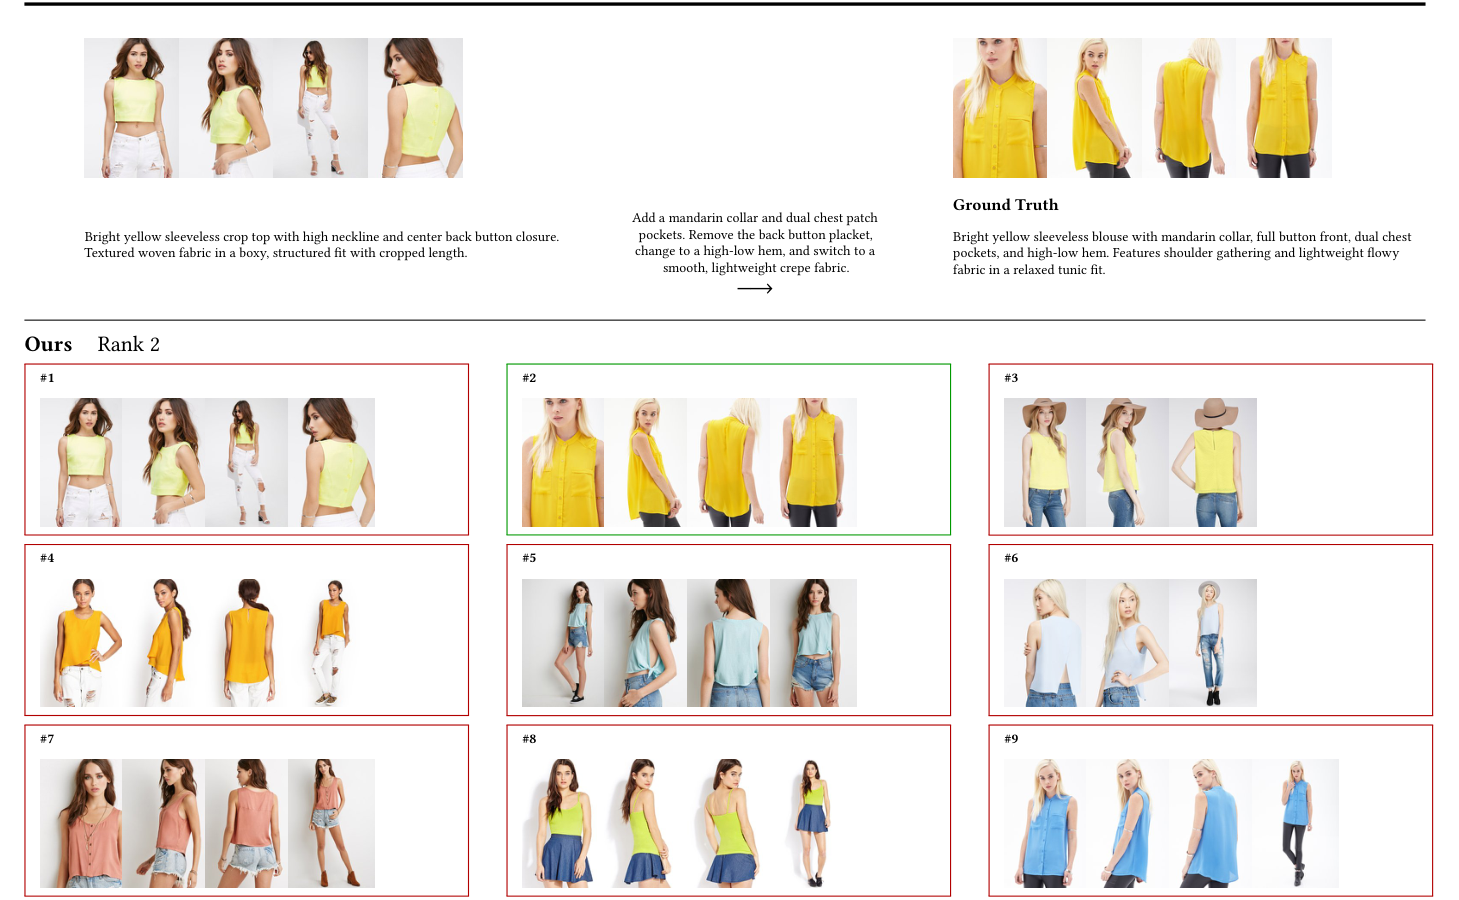
\includegraphics[width=\textwidth]{retrieval_case.png}
\caption{Một ví dụ truy xuất của ProCIR trên DeepFashion: sản phẩm nguồn kèm chú thích (trên trái), văn bản chỉnh sửa (giữa), sản phẩm đích (trên phải) và 9 kết quả đầu tiên (dưới; khung xanh là đích đúng, ở hạng 2). Kết quả hạng 1 trùng với sản phẩm nguồn (nguồn: Mục H, tài liệu bổ sung của~\cite{yuan2026fashionmv}).}
\label{fig:retrieval_case}
\end{figure}

\section{Nhận xét về phương pháp}\label{sec:method-critique}

Từ việc nghiên cứu bài báo và mã nguồn đi kèm, học viên rút ra một số nhận xét sau.

\paragraph{Điểm mạnh.}
\begin{itemize}
    \item \textbf{Định nghĩa bài toán có ý nghĩa thực tiễn rõ ràng.} Đơn vị truy xuất là sản phẩm phù hợp với nhu cầu thương mại điện tử, và công thức suy biến về CIR chuẩn khi $N_P = 1$ giúp bài toán mới tương thích ngược.
    \item \textbf{Pipeline dữ liệu có thiết kế cẩn thận.} Cơ chế đối chiếu 10 ứng viên giải quyết trực tiếp vấn đề mơ hồ đa đáp án đúng; bước lọc ảo giác dựa trên đánh giá thủ công có số liệu cụ thể.
    \item \textbf{Ablation có hệ thống.} 16 cấu hình với chi phí huấn luyện đầy đủ cho phép rút ra các kết luận rõ ràng về vai trò của từng cơ chế, đặc biệt là sự phụ thuộc lẫn nhau giữa MT và Align.
    \item \textbf{Hiệu quả tham số.} Một mô hình 0,8B vượt các mô hình embedding 8B, cho thấy giá trị của thích nghi chuyên biệt so với mở rộng quy mô.
    \item \textbf{Công khai tài nguyên.} Annotation, checkpoint và mã đánh giá đều được phát hành, cho phép tái lập độc lập.
\end{itemize}

\paragraph{Hạn chế và điểm cần làm rõ.}
\begin{itemize}
    \item \textbf{Phụ thuộc vào các mô hình đóng/lớn trong khâu dữ liệu.} Kimi K2.5, Qwen3.5-397B và Gemini 3.1 Flash-Lite đều là mô hình rất lớn; cả triplet lẫn chú thích (được dùng cho Align, CoT, SFT) đều do MLLM sinh, nên chất lượng phụ thuộc hoàn toàn vào các mô hình này, và bộ lọc ảo giác chỉ có recall 36,0\%.
    \item \textbf{Tập đánh giá cũng do mô hình sinh.} Văn bản chỉnh sửa trong tập validation được sinh bởi cùng pipeline với tập huấn luyện; chưa có đánh giá trên truy vấn do người thật viết.
    \item \textbf{Giao thức đánh giá chưa được mô tả đầy đủ.} Bài báo không nêu rõ sản phẩm nguồn có bị loại khỏi danh sách xếp hạng hay không. Đọc mã \texttt{evaluate.py} cho thấy gallery gồm mọi sản phẩm xuất hiện trong các triplet validation, \emph{kể cả sản phẩm nguồn}, và không có bước loại bỏ. Như ví dụ ở Hình~\ref{fig:retrieval_case}, sản phẩm nguồn có thể chiếm hạng 1, làm giảm R@1. Ảnh hưởng của chi tiết này được định lượng ở Chương~\ref{chapter:experiments}.
    \item \textbf{Mã huấn luyện chưa công bố}, nên chưa thể kiểm chứng độc lập các kết quả ablation.
    \item \textbf{Chưa có phân tích về cơ chế tổng hợp đa góc nhìn bên trong mô hình.} ProCIR dựa hoàn toàn vào attention nhân quả để ``tự'' tổng hợp các góc nhìn; bài báo chưa phân tích mô hình chú ý vào góc nhìn nào khi văn bản đề cập đến một chi tiết cụ thể, cũng chưa khảo sát độ bền khi thiếu góc nhìn hay khi thứ tự góc nhìn thay đổi.
\end{itemize}
 % Phương pháp FashionMV / ProCIR
        \newpage
	\chapter{Cơ sở thực nghiệm}\label{chapter:experimental-basis}
\pagestyle{fancy}

Chương này trình bày các thành phần làm nền cho thực nghiệm: các bộ dữ liệu (Mục~\ref{sec:datasets}), phương pháp và giao thức đánh giá (Mục~\ref{sec:evaluation}), và quy trình chuẩn bị dữ liệu ảnh từ nguồn thay thế mà học viên phải xây dựng do nguồn ảnh gốc không khả dụng (Mục~\ref{sec:data-prep}).

\section{Giới thiệu về tập dữ liệu}\label{sec:datasets}

FashionMV chỉ phát hành phần \emph{chú thích văn bản} (triplet và caption, dạng JSONL trên HuggingFace); ảnh sản phẩm phải được tải từ ba bộ dữ liệu gốc. Vì vậy, hiểu rõ đặc điểm của từng bộ gốc là cần thiết để đánh giá ảnh hưởng của nguồn ảnh lên kết quả.

\subsection{DeepFashion (In-shop Clothes Retrieval)}

DeepFashion~\cite{liu2016deepfashion} là bộ dữ liệu thời trang quy mô lớn do Phòng thí nghiệm MMLab (Đại học Trung văn Hồng Kông) công bố năm 2016, gồm nhiều benchmark con. FashionMV sử dụng benchmark \emph{In-shop Clothes Retrieval}, gồm ảnh sản phẩm chụp trong studio của các cửa hàng trực tuyến, mỗi mặt hàng có nhiều ảnh chụp người mẫu từ các góc nhìn khác nhau với tên tệp mang nhãn góc nhìn (ví dụ \texttt{02\_1\_front.jpg}, \texttt{02\_2\_side.jpg}, \texttt{02\_3\_back.jpg}, \texttt{02\_4\_full.jpg}). Mỗi sản phẩm trong FashionMV được định danh bằng đường dẫn thư mục dạng \texttt{WOMEN/Tees\_Tanks/id\_00006581/12}, tức giới tính / danh mục / mã mặt hàng / mã biến thể.

Benchmark này có hai phiên bản ảnh: bản chuẩn đã thu nhỏ và bản độ phân giải cao (\texttt{img\_highres}). Theo bài báo FashionMV, ảnh DeepFashion được dùng có độ phân giải trên $512 \times 512$. Tập validation của FashionMV trên DeepFashion gồm 5.188 triplet và 2.791 sản phẩm -- gallery nhỏ nhất trong ba bộ.

\subsection{Fashion200K}

Fashion200K~\cite{han2017fashion200k} gồm khoảng 200 nghìn ảnh thời trang thu thập từ các trang mua sắm trực tuyến, thuộc năm danh mục (váy liền, áo, quần, chân váy, áo khoác), mỗi ảnh kèm mô tả sản phẩm. Bộ dữ liệu này đã được TIRG~\cite{vo2019tirg} sử dụng như một benchmark CIR mức ảnh với văn bản chỉnh sửa sinh tự động từ khác biệt thuộc tính (``thay \emph{đỏ} bằng \emph{xanh}''). Trong FashionMV, các ảnh cùng mã sản phẩm được gom nhóm thành một sản phẩm đa góc nhìn (thư mục đặt tên theo mã số, ví dụ \texttt{90456812}). Tập validation có 18.499 triplet và 10.720 sản phẩm -- gallery lớn nhất -- với số góc nhìn trung bình thấp nhất ($\sim$3,3 ảnh mỗi sản phẩm).

\subsection{FashionGen}

FashionGen~\cite{rostamzadeh2018fashiongen} là bộ dữ liệu được công bố cho thử thách sinh ảnh thời trang, gồm khoảng 293 nghìn ảnh của khoảng 78 nghìn sản phẩm chụp từ nhiều góc, mỗi sản phẩm kèm mô tả chuyên nghiệp. Ảnh được phân phối dưới dạng tệp HDF5 ở độ phân giải $256 \times 256$; FashionMV dùng tệp \texttt{fashiongen\_256\_256\_validation.h5} cho tập đánh giá. Đây là bộ khó nhất theo bài báo do độ phân giải thấp. Tại thời điểm thực hiện Thực tập, trang tải chính thức của FashionGen \textbf{không còn hoạt động}, và chính kho mã của FashionMV cũng ghi chú rằng tác giả không cung cấp liên kết tải thay thế. Do đó FashionGen nằm ngoài phạm vi đánh giá của báo cáo.

\subsection{Tập validation FashionMV được sử dụng}

Bảng~\ref{tab:val-stats} thống kê tập validation do học viên tính trực tiếp từ tệp \texttt{val\_triplets.jsonl}. Mỗi bản ghi gồm năm trường: \texttt{source\_id}, \texttt{target\_id}, \texttt{dataset}, \texttt{views\_involved} (danh sách góc nhìn mà văn bản chỉnh sửa đề cập) và \texttt{modification\_text\_short}. Đáng chú ý là tập validation công bố \emph{chỉ chứa văn bản chỉnh sửa ngắn}, phù hợp với giao thức chỉ đánh giá bằng văn bản ngắn của bài báo.

\begin{table}[h]
\centering
\caption{Thống kê tập validation FashionMV (tính từ \texttt{val\_triplets.jsonl}).}
\label{tab:val-stats}
\begin{tabular}{lrrr}
\toprule
& DeepFashion & Fashion200K & FashionGen-val \\
\midrule
Số triplet & 5.188 & 18.499 & 9.031 \\
Số sản phẩm (gallery) & 2.791 & 10.720 & 5.292 \\
Triplet / sản phẩm & 1,86 & 1,73 & 1,71 \\
Độ dài văn bản chỉnh sửa (trung vị, từ) & 23 & 24 & 24 \\
\midrule
\multicolumn{4}{l}{\emph{Tổ hợp góc nhìn được đề cập (\texttt{views\_involved})}} \\
sau + trước & 74,2\% & 90,6\% & 71,2\% \\
trước + nghiêng & 15,8\% & 5,6\% & 21,0\% \\
sau + trước + nghiêng & 6,9\% & 1,9\% & 4,5\% \\
khác & 3,1\% & 1,9\% & 3,3\% \\
\bottomrule
\end{tabular}
\end{table}

Có thể thấy hầu hết văn bản chỉnh sửa đề cập đồng thời mặt trước và mặt sau của sản phẩm (từ 71\% đến hơn 90\% tuỳ bộ). Điều này khẳng định về mặt dữ liệu rằng một mô hình chỉ nhìn một ảnh sẽ thiếu thông tin cho phần lớn truy vấn -- chính là động lực của bài toán Multi-View CIR.

\section{Phương pháp đánh giá}\label{sec:evaluation}

\subsection{Độ đo Recall@K}

Độ đo chính của bài toán là \textbf{Recall@K} (R@K): tỷ lệ truy vấn mà sản phẩm đích nằm trong K kết quả đầu tiên của danh sách xếp hạng. Với tập truy vấn $\mathcal{Q}$, gallery $\mathcal{G}$ và $\mathrm{rank}(q)$ là thứ hạng của sản phẩm đích của truy vấn $q$:
\begin{equation}
    \mathrm{R@K} = \frac{1}{|\mathcal{Q}|} \sum_{q \in \mathcal{Q}} \mathbb{1}\big[\mathrm{rank}(q) \le K\big] \times 100\%.
    \label{eq:recall}
\end{equation}
Vì mỗi truy vấn chỉ có đúng một đích, R@K tương đương \emph{hit rate} tại K. Bài báo báo cáo R@5 và R@10; báo cáo này bổ sung R@1 (do mã đánh giá gốc cũng tính R@1) vì R@1 nhạy với vị trí của sản phẩm nguồn trong danh sách xếp hạng (Mục~\ref{sec:source-in-gallery}). Độ tương đồng là cosine giữa các embedding đã chuẩn hoá $L_2$.

\subsection{Giao thức đánh giá của mã nguồn gốc}\label{sec:protocol}

Học viên đọc kỹ mã \texttt{evaluate.py} và gói \texttt{procir} của tác giả để nắm chính xác giao thức. Quy trình gồm ba pha:

\begin{enumerate}
    \item \textbf{Mã hoá gallery.} Lớp \texttt{ProductValDataset} duyệt tệp \texttt{val\_triplets.jsonl} và lấy \emph{tập hợp mọi mã sản phẩm xuất hiện ở vị trí nguồn hoặc đích} của các triplet được chọn. Sản phẩm nào có thư mục ảnh tồn tại sẽ được đưa vào gallery, với tối đa \texttt{MAX\_VIEWS = 5} ảnh đầu tiên theo thứ tự tên tệp. Mỗi sản phẩm được mã hoá một lượt (chỉ ảnh, Hình~\ref{fig:mllm}) để lấy embedding $\mathbf{d}$.
    \item \textbf{Mã hoá truy vấn.} Lớp \texttt{CIRValDataset} giữ lại các triplet mà cả sản phẩm nguồn lẫn đích đều có ảnh. Mỗi truy vấn được dựng thành hội thoại hai lượt (Hình~\ref{fig:two-stage-seq}) với văn bản chỉnh sửa ngắn; mô hình trả về $\mathbf{s}$ (tại \texttt{<emb>} đầu) và $\mathbf{q}$ (tại \texttt{<emb>} cuối). Nếu một sản phẩm nguồn chưa có trong gallery, $\mathbf{s}$ của nó được bổ sung vào gallery (``source reuse'').
    \item \textbf{Tính Recall.} Với mỗi bộ dữ liệu, ma trận tương đồng giữa các $\mathbf{q}$ và toàn bộ gallery của bộ đó được tính, rồi R@1, R@5, R@10 được tính theo~\eqref{eq:recall}.
\end{enumerate}

Ảnh được xử lý với số điểm ảnh trong khoảng $[128^2, 512^2]$ (hằng số \texttt{IMAGE\_MIN\_PIXELS} và \texttt{IMAGE\_MAX\_PIXELS}). Từ giao thức trên, có hai hệ quả quan trọng đối với việc tái lập:

\paragraph{Hệ quả 1 -- Gallery phụ thuộc vào tập triplet được đánh giá.} Gallery không phải một danh mục cố định mà được dựng từ chính các triplet. Nếu chỉ đánh giá trên một mẫu con triplet, gallery tự động co lại tương ứng. Ngoài ra, sản phẩm không có ảnh sẽ biến mất khỏi gallery.

\paragraph{Hệ quả 2 -- Sản phẩm nguồn nằm trong gallery.} Mã không loại sản phẩm nguồn khỏi danh sách xếp hạng của truy vấn. Vì sản phẩm đích thường rất giống sản phẩm nguồn ngoại trừ các chi tiết được chỉnh sửa, sản phẩm nguồn là một ``đối thủ'' mạnh, có thể chiếm hạng 1.

\subsection{Ảnh hưởng của kích thước gallery đến Recall@K}\label{sec:gallery-size-theory}

R@K phụ thuộc trực tiếp vào số lượng sản phẩm gây nhiễu (\emph{distractor}) trong gallery. Một mô hình xếp hạng ngẫu nhiên có R@K kỳ vọng bằng $K / |\mathcal{G}|$. Với một mô hình bất kỳ, nếu coi mỗi distractor có xác suất $p$ (độc lập) được xếp trên đích, thì
\begin{equation}
    \mathbb{E}\big[\#\{\text{distractor xếp trên đích}\}\big] = p\,(|\mathcal{G}| - 1),
\end{equation}
tức là số đối thủ vượt mặt đích tăng tuyến tính theo kích thước gallery. Thu nhỏ gallery $c$ lần sẽ giảm số đối thủ này khoảng $c$ lần, làm R@K tăng lên một cách hệ thống mà không phản ánh năng lực mô hình. Vì vậy, kết quả trên các gallery có kích thước khác nhau \emph{không thể so sánh trực tiếp}, và mọi so sánh giữa các mô hình phải được thực hiện trên \emph{cùng một gallery}. Nguyên tắc này được áp dụng triệt để khi so sánh ProCIR với các baseline ở Chương~\ref{chapter:experiments}.

\section{Chuẩn bị dữ liệu ảnh từ nguồn thay thế}\label{sec:data-prep}

\subsection{Vấn đề với nguồn ảnh gốc}

Kho mã FashionMV hướng dẫn tải ảnh DeepFashion từ trang chính thức của MMLab (qua Google Drive) và ảnh Fashion200K từ kho GitHub của tác giả gốc (cũng dẫn tới Google Drive). Trong quá trình thực hiện, các liên kết Google Drive này chặn công cụ tải tự động do giới hạn hạn mức truy cập của tệp chia sẻ công khai, và việc tải thủ công các tệp nén nhiều GB cũng không ổn định. Như đã nêu, FashionGen hoàn toàn không còn nguồn tải chính thức.

\subsection{Nguồn thay thế trên HuggingFace}

Học viên sử dụng hai bản sao công khai trên HuggingFace do tổ chức Marqo phát hành: \texttt{Marqo/deepfashion-inshop} và \texttt{Marqo/fashion200k}. Cả hai lưu ảnh dưới dạng tệp parquet, mỗi dòng gồm byte ảnh và một mã \texttt{item\_ID}. Học viên viết các script trích xuất (Phụ lục~\ref{chapter:appendix-code}) để ánh xạ \texttt{item\_ID} về mã sản phẩm của FashionMV và dựng lại cấu trúc thư mục \texttt{images/<dataset>/<product\_id>/} mà \texttt{evaluate.py} yêu cầu:
\begin{itemize}
    \item \textbf{DeepFashion}: \texttt{item\_ID} có dạng mã sản phẩm với dấu ``\texttt{/}'' thay bằng ``\texttt{\_}'' cộng hai hậu tố (số thứ tự ảnh và góc nhìn); tiền tố trước hai dấu ``\texttt{\_}'' cuối cùng được so khớp với mã sản phẩm đã chuẩn hoá.
    \item \textbf{Fashion200K}: \texttt{item\_ID} có dạng \texttt{<product\_id>\_<chỉ số ảnh>}; phần trước dấu ``\texttt{\_}'' cuối cùng là mã sản phẩm.
\end{itemize}
Chỉ các ảnh thuộc sản phẩm có mặt trong tập validation mới được trích xuất, giúp giảm dung lượng lưu trữ.

\subsection{Độ phủ dữ liệu}

Bảng~\ref{tab:coverage} tổng hợp độ phủ thu được.

\begin{table}[h]
\centering
\caption{Độ phủ ảnh từ nguồn thay thế so với yêu cầu của tập validation FashionMV.}
\label{tab:coverage}
\begin{tabular}{lrrrrr}
\toprule
Bộ dữ liệu & SP cần & SP có ảnh & Độ phủ SP & Số ảnh & Triplet khả dụng \\
\midrule
DeepFashion & 2.791  & 2.791 & 100\%  & 11.305 & 5.188 / 5.188 (100\%) \\
Fashion200K & 10.720 & 6.908 & 64,4\% & 20.923 & 8.920 / 18.499 (48,2\%) \\
FashionGen  & 5.292  & 0     & 0\%    & 0      & 0 / 9.031 \\
\bottomrule
\end{tabular}
\end{table}

DeepFashion đạt độ phủ đầy đủ (trung bình 4,05 ảnh mỗi sản phẩm). Với Fashion200K, bản sao chỉ chứa ảnh của 6.908 trong 10.720 sản phẩm cần thiết; vì một triplet chỉ khả dụng khi \emph{cả} nguồn và đích đều có ảnh, tỷ lệ triplet khả dụng giảm xuống còn 48,2\% (xấp xỉ bình phương độ phủ sản phẩm, $0{,}644^2 \approx 0{,}41$, cộng thêm ảnh hưởng của việc một số sản phẩm xuất hiện trong nhiều triplet). Các sản phẩm Fashion200K có ảnh trung bình có 3,03 ảnh.

\subsection{Khác biệt về độ phân giải ảnh}\label{sec:resolution}

Học viên kiểm tra kích thước ảnh của nguồn thay thế bằng cách lấy mẫu ngẫu nhiên:
\begin{itemize}
    \item \textbf{DeepFashion (Marqo)}: 300/300 ảnh mẫu có kích thước đúng $224 \times 224$ -- bản sao đã thu nhỏ và cắt vuông toàn bộ ảnh. Trong khi đó, bài báo dùng ảnh trên $512 \times 512$.
    \item \textbf{Fashion200K (Marqo)}: kích thước thay đổi, trung vị $214 \times 449$ (khoảng 98 nghìn điểm ảnh); chỉ 3,9\% ảnh vượt quá $512^2$ điểm ảnh.
\end{itemize}
Theo cấu hình thị giác của Qwen3.5 (Bảng~\ref{tab:qwen35-config}), mỗi token thị giác tương ứng một vùng $32 \times 32$ điểm ảnh. Do đó, một ảnh DeepFashion $224 \times 224$ chỉ tạo ra $7 \times 7 = 49$ token thị giác, trong khi một ảnh độ phân giải cao được giới hạn ở $512^2$ điểm ảnh tạo ra tới khoảng 256 token -- \textbf{gấp khoảng 5 lần}. Với Fashion200K, ảnh thay thế tạo ra trung vị khoảng 96 token mỗi ảnh. Sự chênh lệch này có ý nghĩa đặc biệt vì các văn bản chỉnh sửa trong FashionMV thường đề cập các chi tiết nhỏ (khuy, đường may, khoá kéo, hoạ tiết); với ít token hơn, các chi tiết này có thể không còn phân biệt được. Hệ quả lên kết quả tái lập được phân tích ở Mục~\ref{sec:discussion}.
 % Cơ sở thực nghiệm
        \newpage
	\chapter{Thực nghiệm và đánh giá}\label{chapter:experiments}
\pagestyle{fancy}

Chương này trình bày toàn bộ thực nghiệm của Thực tập 1: thiết lập và quá trình chạy (Mục~\ref{sec:setup}), các nhóm mô hình (Mục~\ref{sec:model-groups}), kết quả tái lập ProCIR (Mục~\ref{sec:repro-results}), kết quả các mô hình cơ sở (Mục~\ref{sec:baseline-results}) và thảo luận (Mục~\ref{sec:discussion}). Mọi số liệu trong chương được ghi nhận từ các tệp kết quả của các lần chạy thực tế (thư mục \texttt{out/} và đầu ra kernel Kaggle).

\section{Thiết lập thực nghiệm}\label{sec:setup}

\subsection{Hạ tầng tính toán}

Học viên không có GPU riêng. Một phép đo thử trên CPU của máy cá nhân cho thấy việc chạy ProCIR trên toàn bộ tập validation DeepFashion sẽ kéo dài nhiều ngày, do mỗi truy vấn đòi hỏi một lượt truyền xuôi của MLLM 0,8B trên chuỗi chứa hàng trăm token thị giác. Do đó, thực nghiệm được chia trên hai môi trường:
\begin{itemize}
    \item \textbf{Kaggle Notebook (GPU miễn phí)} cho ProCIR. Kernel được viết thành script Python và đẩy lên bằng Kaggle API, tự động: cài đặt thư viện (\texttt{transformers}$\ge$5.0, \texttt{huggingface\_hub} 1.33.0, \texttt{pyarrow}), sao chép kho mã FashionMV, tải annotation và checkpoint từ HuggingFace, tải và trích ảnh từ bản sao parquet, rồi gọi \texttt{evaluate.py} nguyên bản. Giới hạn của môi trường là khoảng 12 giờ mỗi phiên và hạn mức khoảng 30 giờ GPU mỗi tuần cho mỗi tài khoản.
    \item \textbf{CPU máy cá nhân} cho các baseline CLIP và FashionCLIP. Các mô hình này nhẹ (ViT-B/32, 49 token mỗi ảnh) nên chạy được trên CPU trong khoảng 10--30 phút cho mỗi lượt mã hoá gallery.
\end{itemize}

\subsection{Quá trình chạy ProCIR trên Kaggle}

Bảng~\ref{tab:kaggle-runs} tóm tắt các phiên bản kernel đã được lưu lại. Với DeepFashion, lần chạy trên toàn bộ tập validation hoàn tất thành công. Với Fashion200K, các lần chạy với cỡ dữ liệu và batch lớn đều không hoàn tất: lần chạy toàn bộ tập vượt quá thời lượng cho phép của phiên, còn lần chạy mẫu 2.000 triplet với batch 48 bị ngắt giữa chừng. Nguyên nhân chính là kiến trúc lai của Qwen3.5 (Mục~\ref{sec:linear-attn}): kernel thành công trên DeepFashion không cài các thư viện \texttt{causal-conv1d} và \texttt{flash-linear-attention}, nên 18 tầng attention tuyến tính chạy bằng triển khai tham chiếu PyTorch chậm; các phiên bản sau có thử cài đặt nhưng không đảm bảo bản biên dịch tương thích với môi trường Kaggle (lệnh cài đặt được đặt ở chế độ không bắt buộc thành công). Lần chạy cuối cùng giảm cỡ mẫu xuống 1.500 triplet và batch xuống 8 để hạn chế cả rủi ro thời gian lẫn bộ nhớ, và đã hoàn tất.

\begin{table}[h]
\centering
\caption{Các phiên bản kernel Kaggle chạy ProCIR.}
\label{tab:kaggle-runs}
\small
\begin{tabular}{llrrl}
\toprule
Kernel & Bộ dữ liệu & Số triplet & Batch & Kết quả \\
\midrule
\texttt{deepfashion} & DeepFashion & 5.188 (toàn bộ) & 32 & Thành công \\
\texttt{f200k} & Fashion200K & 8.920 (toàn bộ khả dụng) & 32 & Không hoàn tất trong phiên \\
\texttt{f200k\_v3} & Fashion200K & 2.000 (mẫu, seed 42) & 48 & Bị ngắt giữa chừng \\
\texttt{f200k\_v4} & Fashion200K & 1.500 (mẫu, seed 42) & 8 & Thành công \\
\bottomrule
\end{tabular}
\end{table}

Phép lấy mẫu dùng \texttt{random.sample} với seed cố định 42 trên danh sách 8.920 triplet khả dụng theo thứ tự tệp gốc. Học viên đã tái hiện lại phép lấy mẫu này và xác nhận một tính chất quan trọng: \textbf{mẫu 1.500 triplet là tập con đúng của mẫu 2.000 triplet} (cả 1.500 triplet đều nằm trong mẫu 2.000). Theo giao thức ở Mục~\ref{sec:protocol}, gallery của lần chạy 1.500 triplet gồm \textbf{2.367 sản phẩm} (1.231 sản phẩm đích khác nhau), trong khi gallery của mẫu 2.000 triplet gồm 2.968 sản phẩm.

\subsection{Thiết lập mô hình cơ sở}\label{sec:baseline-setup}

Vì CLIP và FashionCLIP không được thiết kế cho CIR, truy vấn được tạo bằng chiến lược \textbf{hợp nhất muộn} phổ biến trong các công trình CIR trước thời MLLM:
\begin{equation}
    \mathbf{q} = \mathrm{normalize}\big(\alpha\, \bar{\mathbf{v}}_{src} + (1 - \alpha)\, \mathbf{t}_{mod}\big),
    \label{eq:late-fusion}
\end{equation}
trong đó $\mathbf{t}_{mod}$ là embedding (đã chuẩn hoá $L_2$) của văn bản chỉnh sửa ngắn, và $\bar{\mathbf{v}}_{P}$ là embedding sản phẩm, được tính bằng trung bình (rồi chuẩn hoá) embedding của tối đa 5 ảnh đầu tiên của sản phẩm -- tương ứng chiến lược \textbf{MeanPool} của bài báo và cùng giới hạn \texttt{MAX\_VIEWS} với mã gốc. Gallery được dựng \emph{giống hệt} giao thức của \texttt{evaluate.py}: gồm mọi sản phẩm nguồn và đích của tập triplet được đánh giá, mỗi sản phẩm biểu diễn bởi $\bar{\mathbf{v}}_P$. Hàm tính Recall được viết lại đúng theo \texttt{compute\_recall} của mã gốc. Giá trị mặc định là $\alpha = 0{,}5$; ở Mục~\ref{sec:baseline-results}, học viên khảo sát thêm $\alpha \in \{0; 0{,}25; 0{,}5; 0{,}75; 1\}$.

\section{Các nhóm mô hình thực nghiệm}\label{sec:model-groups}

Bảng~\ref{tab:model-groups} tóm tắt ba nhóm mô hình được so sánh.

\begin{table}[h]
\centering
\caption{Các nhóm mô hình trong thực nghiệm.}
\label{tab:model-groups}
\small
\begin{tabular}{p{3.3cm}p{2.2cm}p{3.4cm}p{4.2cm}}
\toprule
Mô hình & Tham số & Mã hoá đa góc nhìn & Vai trò \\
\midrule
ProCIR (checkpoint MT+Align+SFT) & 0,8B & Joint, hội thoại hai lượt & Mô hình được tái lập \\
FashionCLIP + hợp nhất muộn & $\sim$0,15B & MeanPool & Baseline thích nghi miền \\
CLIP ViT-B/32 + hợp nhất muộn & $\sim$0,15B & MeanPool & Baseline tổng quát \\
Số liệu bài báo (Bảng~\ref{tab:paper-comparison}) & -- & -- & Tham chiếu \\
\bottomrule
\end{tabular}
\end{table}

\paragraph{Nhóm 1 -- ProCIR.} Checkpoint công khai \texttt{yuandaxia/ProCIR} tương ứng cấu hình tốt nhất trong ablation (MT+Align+SFT). Mô hình được chạy bằng mã đánh giá gốc, không chỉnh sửa.

\paragraph{Nhóm 2 -- Baseline zero-shot dựa trên CLIP.} CLIP ViT-B/32 (\texttt{openai/clip-vit-base-patch32}) và FashionCLIP (\texttt{patrickjohncyh/fashion-clip}) cùng kiến trúc, khác nhau ở dữ liệu huấn luyện. So sánh hai mô hình này tách bạch lợi ích của thích nghi miền thời trang; so sánh chúng với ProCIR cho thấy lợi ích của kiến trúc CIR chuyên biệt trên nền MLLM. Hai baseline này gần với nhóm ``CIR một-ảnh + MeanPool'' trong bài báo (CLIP4Cir), nhưng không được huấn luyện trên dữ liệu CIR.

\paragraph{Nhóm 3 -- Số liệu tham chiếu.} Các số liệu do bài báo công bố, dùng để đối chiếu kết quả tái lập.

\section{Kết quả tái lập ProCIR}\label{sec:repro-results}

Bảng~\ref{tab:repro} so sánh kết quả tái lập với số liệu bài báo.

\begin{table}[h]
\centering
\caption{Kết quả ProCIR: bài báo gốc so với tái lập (\%).}
\label{tab:repro}
\begin{tabular}{lcccccrr}
\toprule
& \multicolumn{2}{c}{Bài báo} & \multicolumn{3}{c}{Tái lập} & & \\
\cmidrule(lr){2-3}\cmidrule(lr){4-6}
Bộ dữ liệu & R@5 & R@10 & R@1 & R@5 & R@10 & \#Triplet & Gallery \\
\midrule
DeepFashion & 89,2 & 94,9 & 33,58 & 74,42 & 85,25 & 5.188 & 2.791 \\
Fashion200K & 77,6 & 86,6 & 41,27 & 87,93 & 94,53 & 1.500 & 2.367 \\
FashionGen  & 75,0 & 85,3 & -- & -- & -- & -- & -- \\
\bottomrule
\end{tabular}
\end{table}

\begin{figure}[h]
\centering
\begin{tikzpicture}
\begin{axis}[
    ybar, bar width=13pt, width=0.85\textwidth, height=6cm,
    ymin=0, ymax=105, ylabel={Recall (\%)},
    symbolic x coords={DF R@5, DF R@10, F200K R@5, F200K R@10},
    xtick=data, xticklabel style={font=\small},
    nodes near coords, nodes near coords style={font=\scriptsize},
    legend style={at={(0.5,1.03)}, anchor=south, legend columns=2, font=\small},
    enlarge x limits=0.18
]
\addplot[fill=gray!45] coordinates {(DF R@5,89.2) (DF R@10,94.9) (F200K R@5,77.6) (F200K R@10,86.6)};
\addplot[fill=blue!55] coordinates {(DF R@5,74.42) (DF R@10,85.25) (F200K R@5,87.93) (F200K R@10,94.53)};
\legend{Bài báo (gallery đầy đủ), Tái lập}
\end{axis}
\end{tikzpicture}
\caption{So sánh kết quả ProCIR trong bài báo và kết quả tái lập. Sai lệch theo hai chiều ngược nhau: thấp hơn trên DeepFashion, cao hơn trên Fashion200K.}
\label{fig:repro-bar}
\end{figure}

Có thể thấy kết quả tái lập \emph{lệch theo hai chiều ngược nhau}: trên DeepFashion, R@5 thấp hơn bài báo 14,8 điểm và R@10 thấp hơn 9,7 điểm; trên Fashion200K, R@5 lại \emph{cao hơn} 10,3 điểm và R@10 cao hơn 7,9 điểm. Trung bình hai bộ của kết quả tái lập (R@5 = 81,18; R@10 = 89,89) tình cờ gần với trung bình ba bộ của bài báo (80,6; 88,9), nhưng sự trùng hợp này không có ý nghĩa vì hai sai lệch ngược chiều triệt tiêu nhau và tập dữ liệu khác nhau. Nguyên nhân của từng sai lệch được phân tích ở Mục~\ref{sec:discussion}.

\section{Kết quả các mô hình cơ sở}\label{sec:baseline-results}

\subsection{So sánh trên cùng tập triplet và gallery}

Bảng~\ref{tab:baseline} so sánh ProCIR với hai baseline trên \emph{cùng} tập triplet và \emph{cùng} gallery: toàn bộ 5.188 triplet DeepFashion (gallery 2.791 sản phẩm) và đúng mẫu 1.500 triplet Fashion200K mà ProCIR được đánh giá (gallery 2.367 sản phẩm). Với baseline, báo cáo hai giá trị trọng số hợp nhất: $\alpha = 0{,}5$ (mặc định, trọng số bằng nhau) và $\alpha = 0{,}25$ (giá trị tốt nhất của FashionCLIP trong khảo sát ở Mục~\ref{sec:alpha}). Kết quả của cả hai baseline ở $\alpha = 0{,}5$ trên DeepFashion và trên mẫu 2.000 triplet Fashion200K trùng khớp hoàn toàn với lần chạy đầu bằng script \texttt{baseline\_eval.py}, cho thấy pipeline baseline cho kết quả ổn định.

\begin{table}[h]
\centering
\caption{So sánh ProCIR (tái lập) với các baseline zero-shot trên cùng tập triplet và gallery (\%). Giao thức giữ sản phẩm nguồn trong gallery như mã gốc.}
\label{tab:baseline}
\begin{tabular}{lcccccc}
\toprule
& \multicolumn{3}{c}{DeepFashion (gallery 2.791)} & \multicolumn{3}{c}{Fashion200K (gallery 2.367)} \\
\cmidrule(lr){2-4}\cmidrule(lr){5-7}
Mô hình & R@1 & R@5 & R@10 & R@1 & R@5 & R@10 \\
\midrule
CLIP, $\alpha = 0{,}25$       & 6,40 & 21,53 & 30,47 & 6,07 & 19,60 & 28,73 \\
CLIP, $\alpha = 0{,}5$        & 0,44 & 22,11 & 33,85 & 0,53 & 22,87 & 33,60 \\
FashionCLIP, $\alpha = 0{,}25$ & 23,82 & 55,17 & 67,27 & 18,60 & 51,00 & 62,80 \\
FashionCLIP, $\alpha = 0{,}5$ & 0,87 & 47,96 & 64,42 & 0,13 & 48,33 & 63,00 \\
\midrule
\textbf{ProCIR (tái lập)} & \textbf{33,58} & \textbf{74,42} & \textbf{85,25} & \textbf{41,27} & \textbf{87,93} & \textbf{94,53} \\
\bottomrule
\end{tabular}
\end{table}

Trên cả hai bộ dữ liệu và ở cả hai giá trị $\alpha$, thứ tự hiệu năng là \textbf{CLIP $<$ FashionCLIP $<$ ProCIR}:
\begin{itemize}
    \item \textbf{FashionCLIP vượt CLIP rõ rệt} -- ở $\alpha = 0{,}5$, R@5 tăng từ 22,11 lên 47,96 trên DeepFashion và từ 22,87 lên 48,33 trên Fashion200K. Cùng kiến trúc và cùng cách hợp nhất, khác biệt này hoàn toàn đến từ việc thích nghi miền thời trang của bộ mã hoá.
    \item \textbf{ProCIR vượt xa cả hai baseline} -- trên DeepFashion, R@5 của ProCIR (74,42) cao hơn cấu hình baseline tốt nhất (FashionCLIP, $\alpha = 0{,}25$: 55,17) 19,25 điểm; trên Fashion200K, khoảng cách là 36,93 điểm (87,93 so với 51,00). Vì so sánh được thực hiện trên cùng tập triplet và cùng gallery, khoảng cách này phản ánh trực tiếp năng lực mô hình, không bị nhiễu bởi kích thước gallery.
    \item \textbf{R@1 của baseline gần như bằng 0 ở $\alpha = 0{,}5$}, trong khi R@5 vẫn ở mức vài chục phần trăm. Hiện tượng bất thường này được giải thích ở Mục~\ref{sec:source-in-gallery}.
\end{itemize}

\subsection{Ảnh hưởng của trọng số hợp nhất $\alpha$}\label{sec:alpha}

Hình~\ref{fig:alpha} biểu diễn R@5 trên DeepFashion theo $\alpha$, với $\alpha = 0$ tương ứng truy vấn chỉ bằng văn bản và $\alpha = 1$ tương ứng truy vấn chỉ bằng ảnh nguồn.

\begin{figure}[h]
\centering
\begin{tikzpicture}
\begin{axis}[
    width=0.82\textwidth, height=6.2cm,
    xlabel={Trọng số ảnh nguồn $\alpha$}, ylabel={R@5 trên DeepFashion (\%)},
    xtick={0,0.25,0.5,0.75,1}, xticklabels={0, 0.25, 0.5, 0.75, 1},
    ymin=0, ymax=85, grid=major, grid style={gray!25},
    legend style={font=\scriptsize, at={(0.5,-0.28)}, anchor=north, legend columns=3},
    every axis plot/.append style={thick, mark size=2pt}
]
\addplot[blue!70, mark=*] coordinates {(0,38.90) (0.25,55.17) (0.5,47.96) (0.75,25.98) (1,13.84)};
\addplot[blue!70, dashed, mark=o] coordinates {(0,39.11) (0.25,57.90) (0.5,52.68) (0.75,30.38) (1,16.63)};
\addplot[orange!85!black, mark=square*] coordinates {(0,12.49) (0.25,21.53) (0.5,22.11) (0.75,13.51) (1,8.73)};
\addplot[orange!85!black, dashed, mark=square] coordinates {(0,12.55) (0.25,22.78) (0.5,25.44) (0.75,16.31) (1,10.64)};
\addplot[red!70!black, densely dotted, very thick, mark=none] coordinates {(0,74.42) (1,74.42)};
\legend{FashionCLIP, FashionCLIP (loại nguồn), CLIP, CLIP (loại nguồn), ProCIR (tái lập)}
\end{axis}
\end{tikzpicture}
\caption{R@5 của baseline hợp nhất muộn trên DeepFashion theo trọng số $\alpha$ (nét liền: giao thức gốc, giữ sản phẩm nguồn trong gallery; nét đứt: loại sản phẩm nguồn khỏi danh sách xếp hạng; đường chấm: ProCIR tái lập theo giao thức gốc).}
\label{fig:alpha}
\end{figure}

Ba quan sát rút ra:
\begin{itemize}
    \item \textbf{Văn bản mang nhiều thông tin hơn ảnh nguồn.} Truy vấn chỉ bằng văn bản ($\alpha = 0$) đạt R@5 = 38,90 với FashionCLIP và 12,49 với CLIP, cao hơn so với chỉ dùng ảnh nguồn ($\alpha = 1$: 13,84 và 8,73). Điều này phù hợp với cách FashionMV xây dựng dữ liệu: văn bản chỉnh sửa được sinh để mô tả những đặc điểm phân biệt đích với 9 ứng viên cạnh tranh, nên tự nó đã chứa nhiều thông tin về đích.
    \item \textbf{Kết hợp có lợi, với trọng số vừa phải cho ảnh.} Kết hợp hai nguồn luôn tốt hơn dùng riêng từng nguồn. FashionCLIP đạt tốt nhất ở $\alpha = 0{,}25$; với CLIP, hai giá trị $\alpha = 0{,}25$ và $0{,}5$ cho kết quả xấp xỉ nhau. Khi $\alpha$ vượt quá 0,5, hiệu năng của cả hai mô hình giảm mạnh vì embedding truy vấn bị kéo về sát sản phẩm nguồn.
    \item \textbf{Ngay cả cấu hình baseline tốt nhất vẫn kém ProCIR khoảng 19 điểm R@5.} Phép cộng tuyến tính hai vector không thể biểu diễn các chỉnh sửa có cấu trúc như ``bỏ túi ngực, giữ nguyên màu, thêm khoá kéo ở lưng'', trong khi ProCIR xử lý văn bản trong ngữ cảnh đầy đủ của các token thị giác nhờ attention của MLLM.
\end{itemize}

\section{Thảo luận}\label{sec:discussion}

\subsection{Sai lệch trên DeepFashion: ảnh hưởng của độ phân giải}

Kết quả tái lập trên DeepFashion thấp hơn bài báo 14,8 điểm R@5 dù đánh giá trên \emph{toàn bộ} tập validation với gallery đúng kích thước (2.791 sản phẩm). Vì checkpoint, mã đánh giá, tập triplet và gallery đều giống bài báo, khác biệt có hệ thống duy nhất được xác định là \textbf{nguồn ảnh}: bản sao \texttt{Marqo/deepfashion-inshop} chứa ảnh $224 \times 224$, trong khi bài báo dùng ảnh trên $512 \times 512$. Như đã tính ở Mục~\ref{sec:resolution}, mỗi ảnh $224 \times 224$ chỉ cho 49 token thị giác thay vì khoảng 256 token -- giảm khoảng 5 lần lượng thông tin thị giác mà LLM nhận được. Văn bản chỉnh sửa trong FashionMV thường đề cập các chi tiết nhỏ (khuy cài, đường may, khoá kéo, kiểu cổ), vốn là những thông tin dễ mất nhất khi thu nhỏ ảnh. Ngoài ra, ảnh thay thế có dạng vuông trong khi ảnh gốc có tỷ lệ dọc, và mô hình được huấn luyện trên ảnh độ phân giải cao, nên ảnh đầu vào thấp hơn tạo ra sự lệch phân bố giữa huấn luyện và đánh giá.

Lập luận này phù hợp với chính phân tích của bài báo: FashionGen -- bộ có độ phân giải thấp nhất ($256 \times 256$) -- luôn là bộ khó nhất dù có nhiều góc nhìn nhất. Tuy nhiên, cần lưu ý đây là lập luận dựa trên cơ chế; một thí nghiệm đối chứng trên cùng tập triplet với ảnh gốc độ phân giải cao là cần thiết để khẳng định định lượng.

\subsection{Sai lệch trên Fashion200K: ảnh hưởng của kích thước gallery}

Ngược với DeepFashion, kết quả trên Fashion200K \emph{cao hơn} bài báo 10,3 điểm R@5. Kết quả này \textbf{không} có nghĩa mô hình hoạt động tốt hơn công bố. Theo giao thức ở Mục~\ref{sec:protocol}, gallery được dựng từ chính các triplet được đánh giá; với mẫu 1.500 triplet, gallery chỉ còn 2.367 sản phẩm so với 10.720 sản phẩm trong bài báo -- \textbf{nhỏ hơn 4,5 lần}. Theo phân tích ở Mục~\ref{sec:gallery-size-theory}, số đối thủ có khả năng vượt mặt đích giảm tương ứng, làm R@K tăng một cách hệ thống.

Thực nghiệm baseline cung cấp bằng chứng trực tiếp cho hiệu ứng này. Vì mẫu 1.500 triplet là tập con của mẫu 2.000 triplet, có thể so sánh cùng một mô hình trên hai gallery có kích thước khác nhau (Bảng~\ref{tab:gallery-effect}).

\begin{table}[h]
\centering
\caption{Ảnh hưởng của kích thước gallery lên R@K của cùng một mô hình trên Fashion200K ($\alpha = 0{,}5$, giao thức gốc).}
\label{tab:gallery-effect}
\begin{tabular}{lrrcc}
\toprule
Mô hình & \#Triplet & Gallery & R@5 & R@10 \\
\midrule
FashionCLIP & 2.000 & 2.968 & 44,55 & 59,05 \\
FashionCLIP & 1.500 & 2.367 & 48,33 & 63,00 \\
\midrule
CLIP        & 2.000 & 2.968 & 20,00 & 30,75 \\
CLIP        & 1.500 & 2.367 & 22,87 & 33,60 \\
\bottomrule
\end{tabular}
\end{table}

Chỉ thu nhỏ gallery 1,25 lần (từ 2.968 xuống 2.367 sản phẩm) đã làm R@5 của FashionCLIP tăng 3,78 điểm. Với mức thu nhỏ 4,5 lần so với gallery đầy đủ, việc R@5 của ProCIR cao hơn bài báo khoảng 10 điểm là hoàn toàn có thể giải thích bằng hiệu ứng gallery, \emph{kể cả khi} ảnh thay thế (trung vị $214 \times 449$) cũng có độ phân giải thấp hơn bản gốc và lẽ ra kéo kết quả xuống như ở DeepFashion. Ngoài ra, tập triplet khả dụng (48,2\%) là một tập con chọn lọc theo độ phủ của nguồn ảnh thay thế, có thể thiên lệch nhẹ so với phân bố gốc. Do đó, con số 87,93/94,53 chỉ có giá trị khi so sánh với các mô hình khác \emph{trên cùng gallery} (Bảng~\ref{tab:baseline}), không thể so sánh trực tiếp với 77,6/86,6 của bài báo.

\subsection{Sản phẩm nguồn trong gallery}\label{sec:source-in-gallery}

Hiện tượng R@1 của baseline gần bằng 0 ở $\alpha = 0{,}5$ (Bảng~\ref{tab:baseline}) có nguyên nhân từ Hệ quả 2 của giao thức (Mục~\ref{sec:protocol}): sản phẩm nguồn nằm trong gallery và không bị loại khỏi danh sách xếp hạng. Với hợp nhất muộn, truy vấn chứa trực tiếp embedding của sản phẩm nguồn, nên sản phẩm nguồn có độ tương đồng rất cao với truy vấn. Bảng~\ref{tab:source} định lượng hiện tượng này.

\begin{table}[h]
\centering
\caption{Tỷ lệ truy vấn có sản phẩm nguồn ở hạng 1, và R@K khi giữ / loại sản phẩm nguồn khỏi danh sách xếp hạng (DeepFashion, \%).}
\label{tab:source}
\begin{tabular}{lccccc}
\toprule
& & \multicolumn{2}{c}{R@1} & \multicolumn{2}{c}{R@5} \\
\cmidrule(lr){3-4}\cmidrule(lr){5-6}
Mô hình & Nguồn ở hạng 1 & Giữ & Loại & Giữ & Loại \\
\midrule
CLIP, $\alpha = 0{,}25$        & 30,47 & 6,40 & 8,81 & 21,53 & 22,78 \\
CLIP, $\alpha = 0{,}5$         & 97,84 & 0,44 & 8,91 & 22,11 & 25,44 \\
FashionCLIP, $\alpha = 0{,}25$ & 39,34 & 23,82 & 31,11 & 55,17 & 57,90 \\
FashionCLIP, $\alpha = 0{,}5$  & 97,57 & 0,87 & 21,34 & 47,96 & 52,68 \\
\bottomrule
\end{tabular}
\end{table}

Ở $\alpha = 0{,}5$, sản phẩm nguồn chiếm hạng 1 ở 97,57\% truy vấn với FashionCLIP và 97,84\% với CLIP; khi loại nguồn khỏi danh sách xếp hạng, R@1 của FashionCLIP tăng từ 0,87 lên 21,34. R@5 và R@10 bị ảnh hưởng ít hơn nhiều, vì việc sản phẩm nguồn chiếm một vị trí chỉ đẩy đích lùi đúng một hạng.

Với ProCIR, hiện tượng này cũng tồn tại -- Hình~\ref{fig:retrieval_case} trong tài liệu bổ sung của chính bài báo là một ví dụ ProCIR xếp sản phẩm nguồn ở hạng 1 và đích ở hạng 2. Khoảng cách lớn giữa R@1 (33,58) và R@5 (74,42) của ProCIR trên DeepFashion gợi ý rằng một phần truy vấn có thể bị ảnh hưởng tương tự. Do việc chạy lại ProCIR đòi hỏi GPU, báo cáo chưa định lượng được R@1 của ProCIR khi loại nguồn; đây là một việc cần làm tiếp theo. Điều quan trọng rút ra là: bài báo chỉ báo cáo R@5 và R@10 (ít nhạy với hiện tượng này), nhưng khi so sánh với các công trình dùng giao thức loại nguồn cần đặc biệt lưu ý sự khác biệt về giao thức.

\subsection{Bài học về tái lập}

Quá trình tái lập cho thấy một số yếu tố thường bị bỏ qua nhưng ảnh hưởng mạnh đến kết quả truy xuất:
\begin{itemize}
    \item \textbf{Nguồn và độ phân giải ảnh} -- với MLLM có độ phân giải động, độ phân giải ảnh quyết định trực tiếp số token thị giác; bộ dữ liệu chỉ phát hành annotation mà không kèm ảnh khiến kết quả phụ thuộc vào nguồn ảnh người dùng tự tìm.
    \item \textbf{Kích thước và cách dựng gallery} -- gallery dựng từ chính tập triplet khiến mọi phép lấy mẫu con đều làm thay đổi độ khó của bài toán; kích thước gallery nên luôn được báo cáo kèm kết quả.
    \item \textbf{Chi tiết giao thức} -- việc giữ hay loại sản phẩm nguồn có thể thay đổi R@1 của baseline từ gần 0 lên hơn 20\%.
    \item \textbf{Môi trường phần mềm} -- các kiến trúc mới như attention lai cần kernel chuyên dụng; thiếu kernel không làm sai kết quả nhưng có thể làm thời gian chạy vượt quá giới hạn tài nguyên, buộc phải thu nhỏ thực nghiệm.
\end{itemize}

 % Thực nghiệm và đánh giá
        \newpage
	\chapter{Tổng kết}\label{chapter:conclusion}
\pagestyle{fancy}

\section{Kết quả đạt được}

Thực tập 1 đã hoàn thành ba mục tiêu đề ra ở Chương~\ref{chapter:introduction}.

\paragraph{Về tổng hợp bài báo.} Báo cáo đã trình bày một cách có hệ thống công trình FashionMV~\cite{yuan2026fashionmv}: bài toán Multi-View CIR và hiện tượng khiếm khuyết góc nhìn; pipeline ba giai đoạn xây dựng bộ dữ liệu FashionMV; mô hình ProCIR với ba cơ chế hội thoại hai lượt, căn chỉnh dựa trên chú thích và chuỗi suy luận với loại bỏ tiệm tiến, cùng giai đoạn SFT tuỳ chọn; và các kết quả thực nghiệm gồm so sánh với sáu mô hình hiện có và ablation 16 cấu hình. Công trình được đặt trong bối cảnh rộng hơn qua phần tổng quan lịch sử bài toán CIR (Chương~\ref{chapter:overview}) và cơ sở lý thuyết về Transformer, attention tuyến tính, học tương phản, CLIP và MLLM (Chương~\ref{chapter:background}). Ngoài ra, học viên đã đọc mã nguồn đánh giá để làm rõ những chi tiết giao thức không được nêu trong bài báo, và đưa ra các nhận xét phản biện về phương pháp (Mục~\ref{sec:method-critique}).

\paragraph{Về tái lập thực nghiệm.} Học viên đã xây dựng quy trình thay thế nguồn ảnh gốc không khả dụng bằng các bản sao trên HuggingFace, đạt độ phủ 100\% sản phẩm với DeepFashion và 64,4\% với Fashion200K, và chạy thành công mã đánh giá gốc với checkpoint công khai trên GPU miễn phí của Kaggle. Kết quả tái lập đạt R@5/R@10 = 74,42/85,25 trên toàn bộ 5.188 triplet DeepFashion và 87,93/94,53 trên mẫu 1.500 triplet Fashion200K. Các sai lệch so với bài báo -- thấp hơn trên DeepFashion, cao hơn trên Fashion200K -- đều được truy nguyên đến các nguyên nhân cụ thể và định lượng được: ảnh thay thế DeepFashion chỉ có độ phân giải $224 \times 224$ (cung cấp ít token thị giác hơn khoảng 5 lần so với ảnh gốc), và gallery Fashion200K bị thu nhỏ 4,5 lần do đánh giá trên mẫu con.

\paragraph{Về mô hình cơ sở.} Hai baseline zero-shot CLIP và FashionCLIP được đánh giá trên \emph{đúng} tập triplet và gallery của ProCIR. Thứ tự hiệu năng CLIP $<$ FashionCLIP $<$ ProCIR được quan sát nhất quán trên cả hai bộ dữ liệu, với khoảng cách lớn giữa ProCIR và baseline tốt nhất, khẳng định giá trị của kiến trúc CIR chuyên biệt trên nền MLLM so với hợp nhất muộn tuyến tính. Khảo sát trọng số hợp nhất và phân tích vai trò của sản phẩm nguồn trong gallery cung cấp thêm hiểu biết về giao thức đánh giá mà bài báo gốc chưa đề cập.

\paragraph{Về kinh nghiệm thực tiễn.} Quá trình thực hiện cho thấy tái lập một MLLM có kiến trúc attention lai trên tài nguyên miễn phí là khả thi nhưng đòi hỏi nhiều lần điều chỉnh (cỡ mẫu, batch, thư viện kernel), và nhấn mạnh tầm quan trọng của việc ghi lại đầy đủ các chi tiết như nguồn ảnh, độ phân giải và cách dựng gallery khi báo cáo kết quả truy xuất.

\section{Những hạn chế tồn tại}

\begin{itemize}
    \item \textbf{Chưa đánh giá FashionGen.} Không có nguồn ảnh FashionGen khả dụng, nên chỉ đánh giá được 2/3 bộ dữ liệu của bài báo.
    \item \textbf{Fashion200K chỉ đánh giá trên mẫu con.} Mẫu 1.500/18.499 triplet với gallery 2.367 sản phẩm khiến kết quả trên bộ này không so sánh trực tiếp được với số liệu bài báo; ngoài ra tập triplet khả dụng (48,2\%) đã là một tập con chọn lọc theo độ phủ của nguồn ảnh thay thế.
    \item \textbf{Độ phân giải ảnh thấp hơn bản gốc.} Ảnh DeepFashion thay thế ở $224 \times 224$; tác động của độ phân giải đã được lập luận định lượng qua số token thị giác nhưng chưa được kiểm chứng trực tiếp bằng thực nghiệm đối chứng với ảnh gốc.
    \item \textbf{Không tái lập được quá trình huấn luyện.} Mã huấn luyện chưa được công bố, nên các kết luận ablation của bài báo chưa được kiểm chứng độc lập.
    \item \textbf{Baseline còn đơn giản.} Hai baseline là mô hình zero-shot với hợp nhất muộn; chưa đánh giá các baseline mạnh hơn trong bài báo như SPRC hay Qwen3-VL-Embedding do giới hạn tài nguyên.
    \item \textbf{Ảnh hưởng của việc thiếu kernel tối ưu chưa được kiểm chứng.} Về nguyên tắc, chạy attention tuyến tính bằng triển khai tham chiếu chỉ ảnh hưởng tốc độ, không ảnh hưởng kết quả số học (ngoài sai số dấu phẩy động), nhưng điều này chưa được đối chiếu trực tiếp.
\end{itemize}

\section{Định hướng phát triển}

Từ các kết quả và hạn chế trên, học viên đề xuất các hướng phát triển sau cho giai đoạn Thực tập 2:

\begin{enumerate}
    \item \textbf{Hoàn thiện tái lập.} Tìm nguồn ảnh độ phân giải cao cho DeepFashion và nguồn ảnh FashionGen (qua các kênh học thuật), đánh giá Fashion200K trên gallery đầy đủ khi có tài nguyên GPU phù hợp, và chạy đối chứng cùng một tập triplet ở hai độ phân giải để định lượng trực tiếp ảnh hưởng của độ phân giải.
    \item \textbf{Chuẩn hoá giao thức đánh giá.} Báo cáo song song kết quả có và không loại sản phẩm nguồn khỏi danh sách xếp hạng, và luôn báo cáo kèm kích thước gallery.
    \item \textbf{Phân tích cơ chế tổng hợp đa góc nhìn.} Khảo sát bản đồ attention của ProCIR để xem mô hình chú ý vào góc nhìn nào khi văn bản đề cập một chi tiết (ví dụ phần lưng), cũng như độ bền của mô hình khi thiếu góc nhìn, khi đảo thứ tự góc nhìn hoặc khi chỉ có một ảnh.
    \item \textbf{Đề xuất cải tiến.} Dựa trên các phân tích trên, nghiên cứu cơ chế tổng hợp đa góc nhìn có nhận biết góc nhìn (\emph{view-aware}) -- ví dụ gắn nhãn góc nhìn tường minh cho từng ảnh hoặc dùng trường \texttt{views\_involved} làm tín hiệu giám sát phụ -- nhằm giải quyết trực tiếp hơn hiện tượng khiếm khuyết góc nhìn, theo hướng đã nêu trong đề cương nghiên cứu.
\end{enumerate}

\section{Kế hoạch và tiến độ thực hiện}

Thực tập 1 được thực hiện trong bốn tuần, từ ngày 07/09/2026 đến ngày 03/10/2026, theo sáu nhóm công việc: khảo sát tài liệu, nghiên cứu bài báo FashionMV, viết đề cương nghiên cứu, chuẩn bị dữ liệu và môi trường, thực nghiệm, và viết báo cáo (Hình~\ref{fig:timeline}). Toàn bộ công việc do học viên thực hiện cá nhân dưới sự hướng dẫn của giảng viên.

\begin{figure}[h]
\centering
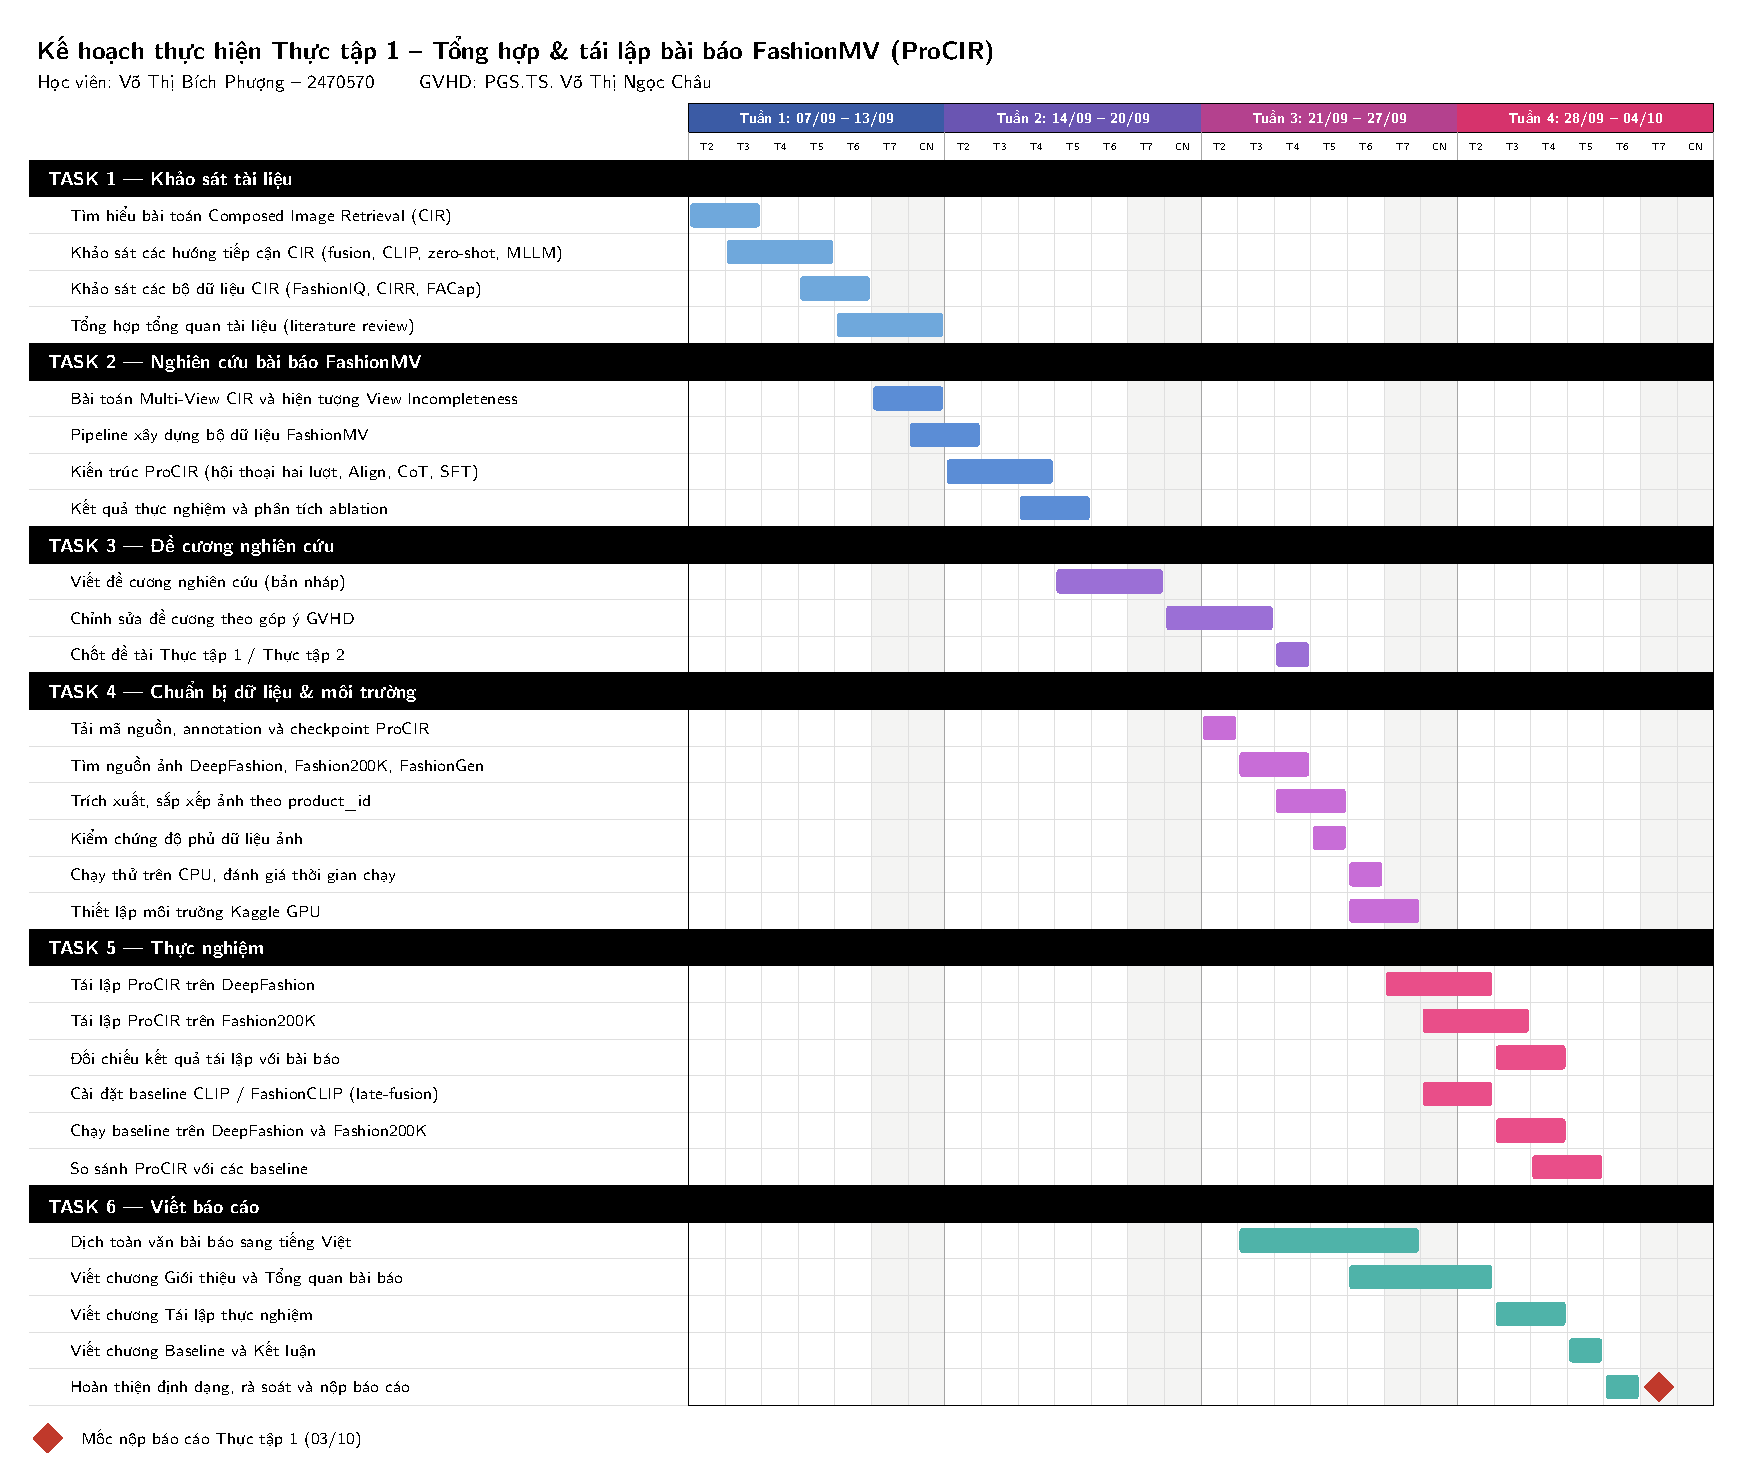
\includegraphics[width=\textwidth]{timeline_tt1.pdf}
\caption{Kế hoạch và tiến độ thực hiện Thực tập 1.}
\label{fig:timeline}
\end{figure}
 % Tổng kết
        \newpage

	\appendix
		\chapter{Danh mục mã nguồn thực nghiệm}\label{chapter:appendix-code}
\pagestyle{fancy}

Toàn bộ script do học viên viết để thực hiện thực nghiệm nằm trong thư mục \texttt{scripts/} đi kèm báo cáo; kết quả thô (tệp JSON và log) nằm trong thư mục \texttt{out/}. Mã đánh giá ProCIR (\texttt{evaluate.py} và gói \texttt{procir}) là mã gốc của tác giả tại \url{https://github.com/yuandaxia2001/FashionMV} và được sử dụng nguyên trạng, không chỉnh sửa. Bảng~\ref{tab:scripts} liệt kê chức năng của từng script.

\begin{table}[h]
\centering
\caption{Danh mục script sử dụng trong thực nghiệm.}
\label{tab:scripts}
\small
\begin{tabular}{p{4.6cm}p{6.4cm}l}
\toprule
Tệp & Chức năng & Môi trường \\
\midrule
\texttt{extract\_deepfashion.py} & Trích ảnh DeepFashion từ parquet \texttt{Marqo/deepfashion-inshop}, dựng thư mục theo mã sản phẩm FashionMV & CPU cục bộ \\
\texttt{extract\_f200k.py} & Trích ảnh Fashion200K từ parquet \texttt{Marqo/fashion200k}, thống kê độ phủ & CPU cục bộ \\
\texttt{kaggle\_script\_deepfashion.py} & Kernel Kaggle: tải annotation, checkpoint, ảnh; chạy \texttt{evaluate.py} trên toàn bộ 5.188 triplet DeepFashion (batch 32) & Kaggle GPU \\
\texttt{kaggle\_script\_f200k\_v4.py} & Kernel Kaggle: lấy mẫu 1.500 triplet Fashion200K khả dụng (seed 42), chạy \texttt{evaluate.py} (batch 8) & Kaggle GPU \\
\texttt{kernel-metadata\_*.json} & Cấu hình kernel Kaggle (bật GPU và Internet) & Kaggle \\
\texttt{baseline\_eval.py} & Baseline CLIP/FashionCLIP hợp nhất muộn ($\alpha = 0{,}5$), lần chạy đầu (Fashion200K mẫu 2.000) & CPU cục bộ \\
\texttt{baseline\_ext.py} & Baseline mở rộng: cùng tập triplet/gallery với ProCIR, khảo sát $\alpha$, đánh giá có/không loại sản phẩm nguồn & CPU cục bộ \\
\bottomrule
\end{tabular}
\end{table}

Để tái lập kết quả ProCIR, chỉ cần đẩy kernel lên Kaggle bằng lệnh \texttt{kaggle kernels push} với tệp metadata tương ứng; kernel tự tải mọi tài nguyên cần thiết từ HuggingFace và GitHub. Để tái lập kết quả baseline, chạy \texttt{extract\_*.py} để dựng thư mục ảnh rồi chạy \texttt{python baseline\_ext.py --model <tên mô hình>} với \texttt{openai/clip-vit-base-patch32} hoặc \texttt{patrickjohncyh/fashion-clip}.


%%%%%%%%%%%%%%%%%%%%%%%%%%%%%%%%%%%%%%%%%%%%%%
%%%%% TAIL: Tài liệu tham khảo
%%%%%%%%%%%%%%%%%%%%%%%%%%%%%%%%%%%%%%%%%%%%%%
\backmatter
    \cleardoublepage
    \phantomsection
    \addcontentsline{toc}{chapter}{Tài liệu tham khảo}
    \bibliographystyle{references/IEEEtran}
    \bibliography{references/refs}
%     \chapter*{Phần lý lịch trích ngang}
\addcontentsline{toc}{chapter}{Phần lý lịch trích ngang}
\markboth{Phần lý lịch trích ngang}{Phần lý lịch trích ngang}
\pagestyle{fancy}

\vspace{0.5cm}
\begin{itemize}
    \item[] Họ và tên: Võ Thị Bích Phượng \hfill MSHV: 2470570
    \vspace{0.2cm}
    \item[] \makebox[0.6\linewidth][l]{Ngày, tháng, năm sinh: \dotfill} Nơi sinh: \dotfill
    \vspace{0.2cm}
    \item[] Địa chỉ liên lạc: Thành phố Hồ Chí Minh
    \vspace{0.2cm}
    \item[] Email: vbichphuon928@gmail.com
\end{itemize}

\section*{Quá trình đào tạo}
\begin{itemize}
    \item \textbf{9/2019 -- 12/2023}: Sinh viên ngành Công nghệ Thông tin, Trường Đại học Giao thông Vận tải TP. Hồ Chí Minh.
    \item \textbf{12/2024 -- nay}: Học viên cao học ngành Khoa học Máy tính, Khoa Khoa học \& Kỹ thuật Máy tính, Trường Đại học Bách Khoa -- ĐHQG TP.HCM.
\end{itemize}

\section*{Quá trình công tác}
\begin{itemize}
    \item \textbf{8/2024 -- nay}: Kỹ sư Phần mềm, PPJ Group, TP. Hồ Chí Minh.
\end{itemize}


\end{document}
